\section{Morse-Theoretic Atiyah-Hirzebruch Spectralsequence}
\subsection{Conley index}
This is just a short summary. Prooves are omitted and the goal is to remaind ourself of the definitinos. 
\begin{definition}[Compact invariant isolated subset]
	For a flow $\phi_t:M\to M$ on a locally compact metric space we call a subset $S\subseteq M$ \textbf{invariant subspace} if and only if $\phi_t(S)=S$ for all $t\in \R$. For any subset $N\subseteq M$ we define the \textbf{maximal invariant subset}
	\begin{align*}
		I(N)&=\{x\in N|~ \phi_t(x)\in N \forall t\in \R\}\\
		&=\bigcap_{t\in \R} \phi_t(N).
	\end{align*} A \textbf{compact invariant subset} $S$ is called \textbf{isolated}, if a compact neighborhood $N$ exists, such that $I(N)=S$.
\end{definition}
\begin{definition}[Index pairs] \label{def: index pairs}
	Let $S$ be an isolated compact invariant subset. A topological pair $(N,L)$ of compact subsets of $M$ where $L\subseteq N$ is called an \textbf{index pair of }S, if it satisfies the following:
	\begin{enumerate}
		\item $S=I(\overline{N\setminus L})\subseteq (\mathring{N\setminus L})$.
		\item  $x\in L$ and $\phi_{[0,t]}(x)\subseteq N$ implies that  $\phi_{[0,t]}(x)\subseteq L$. We call $L$ \textbf{positively invariant in } $N$. Here $\phi_{[0,t]}(x)\coloneq\{ \phi_{\tilde{t}}(x)|\tilde{t}\in [0,t]\}$.
		\item For all $x\in N$ such that a $t$ exists, with $\phi_t(x)\not\in N$, there exists a $t'$ with $\phi_{[0,t']}(x)\subseteq N$ and $\phi_{t'}(x)\in L$.
	\end{enumerate}
	This definition captures how the flow lines leave the invariant space $S$. Due to the third property we call $L$ the \textbf{exit set}.
\end{definition}


\begin{definition}[Regular index pairs]
	We call an index pair $(N,L)$ \textbf{regular} if and only if the inclusion $I: L \hookrightarrow N$ is a cofibration.
\end{definition}
\begin{theorem}[Homotopy equivalence of index pairs] \label{thm: Homotopy equivalence of index pairs}
	If $S$ is an isolated compact invariant set and $(N,L)$ and $(\tilde{N},\tilde{L})$ are two index pairs of $S$. Then $N/L$ and $\tilde{N}/\tilde{L}$ are homotopy equivalent as pointed spaces.
\end{theorem}


\begin{remark}[Critical points as isolated compact invariant subsets] \label{ex: Critical points as isolated compact invariant subsets}
	Let ${f:M\to \R}$ be a Morse function on a smooth Riemannian manifold $(M,g)$. Let $q\in \Crit_k(f)$. Around $q$ we have Morse charts $\phi:U \to T_qM$ (after identifying $q_i$ and $\partial q_i$) where  ${\phi(W(q\to)\cap U)\subseteq T_q^{u}M}$ and ${\phi(W(\to q)\cap U)\subseteq T_q^{s}M}$. With this we can define the balls:
	\begin{align*}
		D^{s}_\epsilon &~=~\{v\in T_q^{s}M | \norm{v}\leq \epsilon \}, \\
		D^{u}_\epsilon &~=~\{v\in T_q^{u }M | \norm{v}\leq \epsilon \}. 
	\end{align*} They give rise to the index pair $N_q\coloneq\phi^{-1}( D^{s }\times  D^{u })$ and $L_q=\phi^{-1}( D^{ s}\times \partial D^{u})$. This index pair is in fact regular, since $(N_q,L_q)\cong  (D^{ s}\times  D^{u }, D^{s}\times \partial D^{u}) \cong (D^{u}_{\epsilon},\partial D^{u}_{\epsilon} )$. Now we know the K-group of such a pair:
	\begin{align} \label{eq: homology of indexx pair of critical point}
		K^i(N_q,L_q)=K^i(D^{k},\partial D^{k})=\begin{cases}
			\Z & \text{if } i-k\in 2\N,\\
			0& \text{else. }
		\end{cases}
	\end{align}
	Notice that for $k=0$ we need to consider $\partial D^k=\emptyset$, to get an index pair. That's why we let $\partial$ denote the manifold boundary insted of the topological boundary. However, now we can identify for all $k$: \begin{equation} \label{ kritical points as direct sum of homology groups}
		C^{k}(M,\mathfrak{A},\tilde{K}^{l}(pt)=\bigoplus_{ \Crit_k(f)} \Z \cong \bigoplus_{q\in \Crit_k(f)} K^k(N_q,L_q;\Z).
	\end{equation}
\end{remark}
\begin{remark}
		Furthermore, this isomorphism 
		\begin{equation} \label{ kritical points as direct sum of homology groups}
			C^{k}(M,\mathfrak{A},\tilde{K}^{l}(pt)=\bigoplus_{ \Crit_k(f)} \Z \cong \bigoplus_{q\in \Crit_k(f)} K^k(N_q,L_q;\Z).
		\end{equation}
		can be made canonically, using orientations: Let $q$ be a critical point in index $\lambda_q$. Let $\mathfrak{b}$ be a ordered basis of $T^u_qM$. Let $\psi$ be a refined Morse chart arround $q$, such that the induced basis in $T_qM=T^u_qM\oplus T^u_qM$ projects onto a a basis of the first factor $T^u_qM$ that is compatible with $\mathfrak{b}$. Using this Morse chart do define the generator of the regular index pair of $q$ gives a unique generator.
\end{remark}
\begin{proof}
	Let $\psi_1$ and $\psi_2$ be two such Morse charts. Notice that they only differ by order of the directions and their signs, meaning that for all $i$ there is a $j$ such that $\psi_1^{-1}(e_i)=\pm \psi_2{-1}(e_j)$.Hence, viewed as maps into the tangent space we have that $\psi_1(N_p,L_q)=\psi_1(N_p,L_q)\subseteq T_qM$. We define $B^{\lambda_{q}}_{\epsilon}(0)\subseteq \R^{\lambda_q}$ to be the sphere. The generator of $\psi_1(N_p,L_q)$ comes as the pullback of the canonical bott generator of $K^i(B^{\lambda_{q}}_{\epsilon}(0),\partial B^{\lambda_{q}}_{\epsilon}(0))$ via the basis map after the collapse map $c:(D^{ s}\times  D^{u }, D^{s}\times \partial D^{u}) \cong (D^{u}_{\epsilon},\partial D^{u}_{\epsilon} )$. Let $\alpha$ be a generator of $\psi_1(N_p,L_q)$ induced from the basis $\mathfrak{b_1}$ that comes from $\psi_1$. I.e. 
	\begin{equation*}
		\alpha=\left( B_{\mathfrak{b}_1}\circ c\right)^*(\beta)
	\end{equation*} By assumption, the map $ B_{\mathfrak{b}_1}\circ  B_{\mathfrak{b}}^{-1}$ has determinant one. Hence it is homotopic to the identity, and this homotopy can be reduced to a well defined homotopy on the quotient space $\left(D^{u}_{\epsilon}\middle/ \partial D^{u}_{\epsilon} \right)$. Hence
	\begin{equation*}
		\alpha=\left( B_{\mathfrak{b}}\circ c\right)^*(\beta)
	\end{equation*} And thereby, the generacd tor only depends on $\mathfrak{b}$ concluding the proof.
\end{proof}

\begin{example}[A Map of Homology Groups]
	Let $f:M\to \R$ be a Morse Smale function on a smooth compact Riemannian manifold $(M,g)$. Let $q\in \Crit_k(f)$ and $p\in \Crit_{k-1}(f)$. Assume for a moment we already have an isolated regular compact index pair $(N_2,N_0)$ of $S=W(p\to q)\cup\{p,q\}$. 
	For a $c\in (f(p),f(q))$ we set $N_1=N_0\cup (N_2 \cap M^c)$, where $M^c$ is the sublevel set. Clearly now $(N_2,N_1)$ is an index pair for $q$ and $(N_1,N_0)$ is a pair for $p$. Assuming we have regular index pairs $(N_q.L_q)$ and $(N_p,L_p)$ for $p,q$ we can now define a map:
	\begin{align*}
		\Delta^k(q \to p):K^{k-1}(N_p,L_p) \to  K^k(N_q,L_q) 
	\end{align*} as the composition:
	\begin{center}
% https://tikzcd.yichuanshen.de/#N4Igdg9gJgpgziAXAbVABwnAlgFyxMJZAZgBoAGAXVJADcBDAGwFcYkQBpAPQGsAKAHIB9AI6kAMqIDcAHRkAtAJQgAvqXSZc+QigBMFanSat23fsP3CAjLIXK1G7HgJErBmgxZtEnLsB4AtFYqgkJuwuS2SqrqIBhO2kTk7kZepn6BwaFoEkJoUfaGMFAA5vBEoABmAE4QALZIbiA4EEjJqSY+cgDGBCUxVbUNiPrNrYhNnp0gcrCMOPRCwDjVWGiMMCoDIDX1SGRjSKNT3jMyvWD9KpQqQA
\begin{tikzcd}
	{K^{k-1}(N_p,L_p;\Z)} \arrow[r, "\cong"] & {K^{k-1}(N_1,N_0;\Z)} \arrow[r, "\delta_{triple}"] & {K^k(N_2,N_1;\Z)} \arrow[r, "\cong"] & {K^k(N_q,L_q;\Z)}
\end{tikzcd}
	\end{center} where $\delta_{triple}$ is the connecting homomorphism, and the other two maps are induced by the homotopic equivalence of two index pairs corresponding to the same isolated compact invariant subset. Putting all together we can define a morphism:
	\begin{align}\label{equation: definition of boundary operator for filtrations}
		\Delta^k:\bigoplus_{p\in \Crit_{k-1}(f)}K^{k-1}(N_p,L_p) \to \bigoplus_{q\in \Crit_k(f)}K^k(N_q,L_q)
	\end{align}
\end{example}






\begin{definition}[Regular index pairs and a filtration on $M$] \label{def: Regular index pairs and a filtration on M } \label{def: Regular index pairs and a filtration on M}
	As always let $f:M\to \R$ be a Morse-Smale function on a compact smooth Riemannian manifold $(M,g)$ of dimension $m$. Let $\phi_t:M\to M$ be the flow given by $-\grad f$. For $0\leq j\leq k\leq m$ define:
	\begin{align*}
		W(k,j)=\bigcup_{j\leq \lambda_p \leq \lambda_q\leq k} W(q \to p).
	\end{align*}We know that this space is compact\todo{reference}. Assume that $N$ is a compact neighbourhood of $W(k,j)$, such that $\Crit(f)\cap N=\Crit(f)\cap W(k , j)$, meaning that $N$ does not contain any new critical points. Then the biggest invariant subspace from definition \ref{def: index pairs} is
	\begin{align*}
		I(N)\coloneq\{x\in N| \phi_t(x)\in N \forall t \in \R \}=W(j,k).
	\end{align*} This follows from every gradient flow line starting and ending in a critical point.  Therefore, $W(k,j)$ is an isolated compact invariant set. By a corollary of the lambda lemma \todo{reference} we know that 
	\begin{align*}
		W^{s}_{j}&~\coloneq~ \bigcup_{j\leq \lambda_p}W(\to p)\\
		W^{u}_{j}&~\coloneq~\bigcup_{\lambda_p\leq j}W(p \to )\,
	\end{align*}
	for all $j=0,...,m$ are compact as they are finite unions of compact sets. Now we define $N_m\coloneq M$ and choose a cofibered compact neighbourhood $N_{m-1}$ of $W^{p\to }_{m-1}$ that is positively invariant and satisfies $N_{m-1}\cap W^{\to p}_m=\emptyset$
	One could for example define:
	\begin{align*}
		N_{m-1}\coloneq N_m \setminus \Big(\bigcup_{q\in \Crit_m(f)}  \mathring{N_q}\Big),
	\end{align*} where $N_q$ is taken from example \ref{ex: Critical points as isolated compact invariant subsets}. Once we check that $N_{m-1}$ is an exit set with respect to $N_m$ we can conclude that $(N_m,N_{m-1})$ is a regular index pair for $\Crit_m(f)$. The first statement is clear, since every gradient line starting in $N_m\setminus N_{m-1}$ has to pass through $N_{m-1}$, as they go towards other critical points. This tells us that they have to leave $N_m\setminus N_{m-1}$, which is enclosed by $N_{m-1}$. The second thing to check can be done by showing that there is a neighbourhood $U\subset N_M$ of $N_{m-1}$ that deforms to $N_{m-1}$. For this notice that each $N_q$ with $\lambda_q=m$ is homeomorphic to $D^m$. Now choose a open neighbourhood $U_q$ in the disc of its boundary. By definition this retracts to the boundary with a retraction induced by the flow. And finally define $U\coloneq N_{m-1}\cap_{q\in \Crit_m(f)} U_q$. This retracts to $N_{m-1}$ telling us that our index pair is indeed regular. 
	
	Now we want to inductively define a filtration: 
	For this we choose a compact cofibered neighborhood $N_{m-2}$ of $W^{u}_{m-2}$ that is positifely invariant in $N_{m-1}$ and has an empty intersection with $W^{\to p}_{m-1}$. This can be done similar to the construction of $N_{m-1}$ but instead of cutting out neighbourhoods if $q\in \Crit_{m}(f)$, we can cut out tubular neighborhoods of $W^{s}_{m-1}$.\todo{Referenz Dietmar Salamon} By iterating this process we get a filtration: 
	\begin{equation} \label{eq: Filtration conley}
		\emptyset=:N_{-1}\subset N_0\subset N_1\subset \cdots \subset N_{m-1}\subset N_m=M,
	\end{equation} such that $(N_k,N_{j-1})$ is a regular index pair for $W(k,j)$ for all $0\leq j \leq k\leq m$.
\end{definition}
\subsection{The Spectral sequence}

\begin{definition} Let $M$ be a smooth manifold with Morse data and \begin{equation*}
		\emptyset=:N_{-1}\subset N_0\subset N_1\subset \cdots \subset N_{m-1}\subset N_m=M,
	\end{equation*} be a filtrations constructed in \ref{def: Regular index pairs and a filtration on M}. Then we define the Groups
	\begin{equation*}
		E^{p,q}_r(M)\coloneq \frac{\ker\big[K^{p+q}(N_{p+r-1},N_{p-r})\to K^{p+q}(N_{p-1},N_{p-r})  \big]}{\ker\big[K^{p+q}(N_{p+r-1},N_{p-r})\to K^{p+q}(N_{p},N_{p-r})\big]} \, .
	\end{equation*} To define a boundary operator, we proceed as follows:
	The following diagram commutes (by naturality of the boundary in the triple sequence).
	\begin{center}
		% https://tikzcd.yichuanshen.de/#N4Igdg9gJgpgziAXAbVABwnAlgFyxMJZABgBpiBdUkANwEMAbAVxiRAGkA9YNAagEcAvgAoAcgH0evAE4BaAIyDSEnrOmCAlCCXpMufIRTzyVWoxZsuUoWMlolKtGs3bSu7HgJEy80-WasiBzcfPy8irZSAExyisp2MgouOiAYHgZExr7U-hZBVqHhIo68MUnxPMluqXqehshRpNlmAZYhAkWRfLEOdsmmMFAA5vBEoABm0hAAtkhkIDgQSMYteSAAOuuMaAAWdK4TU7OI84tIjauBG+uwDDh0nABUkjjSWGgMMIIHIJMz59QzogAMw5cxXTYAIxg9x+f2OKyBoMubE2t3uTxebw+XzhRyQyKBABZBBRBEA
		\begin{tikzcd}
			{K^{p+q}(N_{p+r-1},N_{p-r})} \arrow[r, "\alpha"] \arrow[d, "\delta^*_{triple}"] & {K^{p+q}(N_{p},N_{p-r})} \arrow[d, "\delta^*_{triple}"] &                              \\
			{K^{p+q+1}(N_{p+2r-1},N_{p+r-1})} \arrow[r, "\beta"]                            & {K^{p+q+1}(N_{p+2r-1},N_{p})} \arrow[r]                 & {K^{p+q+1}(N_{p+r-1},N_{p})}
		\end{tikzcd}
	\end{center} Hence, $\beta\circ \delta^*_{triple}$ factors over ${K^{p+q}(N_{p+r-1},N_{p-r})}\slash \ker \alpha$ and because the bottom row is exact (by the triple sequence) we have get a map 
	\begin{equation*}
		{K^{p+q}(N_{p+r-1},N_{p-r})}\slash \ker \alpha \to \ker\big[K_{p+q+1}(N_{p+2r-1},N_{p})\to K^{p+q+1}(N_{p+r-1},N_{p})  \big]
	\end{equation*} Now since ${K^{p+q}(N_{p+r-1},N_{p-r})}\supseteq \ker\big[K^{p+q}(N_{p+r-1},N_{p-r})\to K^{p+q}(N_{p-1},N_{p-r})  \big]$ we can restrict the domain and furthermore compose with the quotient map to get a well-defined map
	\begin{align*}
		d_r^{p,q}: ~E^{p,q}_r &  \to E^{p+r,q-r+1}_{r}\\
		[x]                   &  \mapsto [\beta\circ \delta^*_{triple}(x)]
	\end{align*}
\end{definition}
\begin{corollary}[The first page]
	We start by analysing the first page
	\begin{align*}
		E^{p,q}_1(M)\coloneq\frac{\ker\big[K^{p+q}(N_{p},N_{p-1})\to K^{p+q}(N_{p-1},N_{p-1})  \big]}{\ker\big[\underbrace{K^{p+q}(N_{p},N_{p-1})\to K^{p+q}(N_{p},N_{p-1})}_{\id}\big]} &\cong K^{p+q}(N_{p},N_{p-1})\\
		&=\tilde{K}^{p+q}(N_p\slash N_{p-1})
	\end{align*}
	Now since $(N_p,N_{p-1})$ is a regular index pair for $\Crit_p(f)$ we have a flow induced homotopiy equivalentce:
	
	\begin{equation*}
		N_p\slash N_{p-1}
		\simeq          \big(\bigcup_{w\in Crit_p(f)}D^u_\epsilon(w)\big) \slash (\bigcup_{w\in Crit_p(f)} \partial D^u_\epsilon(w)\big)
		\cong           \bigvee_{w\in \Crit_p(f)}S^p
	\end{equation*} Here, we use the definitions from above
	\begin{align*}
		D^{u}_\epsilon (w)&~\coloneq~ \phi_w^{-1} \big(\{v\in T_w^{u }M | \norm{v}\leq \epsilon \} \big), 
	\end{align*}and the last isomorphism is induced by orientations in the unstable manifolds. We can continue our inspection:
	\begin{align*}
		E^{p,q}_1&\cong \tilde{K}^{p+q}(N_p\slash N_{p-1})\\
		&\cong \bigoplus_{w\in \Crit_p(f)}\tilde{K}^q(pt)=C^k(M,f,g,\mathfrak{o};\tilde{K}^q(pt))\\
	\end{align*} In sum we have the chain of horizontal isomorphisms: 
	\begin{center}
		% https://tikzcd.yichuanshen.de/#N4Igdg9gJgpgziAXAbVABwnAlgFyxMJZABgBpiBdUkANwEMAbAVxiRAFEA9YNUgRwC+AfQCMIAaXSZc+QihHkqtRizYAdNXgaxgAaQHc0AakEAKAHJC0GuAzpwAFgAJLPALQiBASnGSQGbDwCIgAmRWp6ZlZEEA0AIywAcwg0ZjghYAB3DSwwJw0AYQAnXCtTADMvAQ0tHX1OPlM0HB8JKUDZIgBmcOUotgLDAVMAWVINAFs6HAdyoroAa2AAQQkarG0YPQNG5q9WvwCZYJQyESVI1RiuHiMFQVFfduO5ZAVziJVo2M0NuoNbiITMNXMZPDY7I4XBk0N4nv5pEFXmEPn0rj8EslUkx0lkcnlCiUcDC7sNKtVfpttg0mi14Uckd1SKjLt9BoDhmNJtNZvMlqtxpT-jS9q0lDAoIl4ERQHMIBMkGQQDgIEgFGjvhpGGgHHR4XKFYh1SqkGENeo1HEYDg9W0QAbFdQTYgACyffoxKCiQz8AT6orytVO1WIACsdodiDNzoAbBGA4aesqQwB2eOB13BpCh93orUMHV0ADk-ozOeTSBjuc1lutxdLiazUfThpTTbjFAEQA
		\begin{tikzcd}
			{E^{p,q}_1} \arrow[r, "\alpha"] \arrow[d, "{d_1^{p,q}}"] & \tilde{K}^{p+q}(N_p\slash N_{p-1}) \arrow[r, "\beta"] \arrow[d] & \bigoplus_{w\in \Crit_p(f)}\tilde{K}^q(pt) \arrow[d] & {C^{p}(M,\mathfrak{A},\tilde{K}^q(pt))} \arrow[d] \arrow[l] \\
			{E^{p+1,q}_1} \arrow[r, "\alpha'"]                       & \tilde{K}^{p+1+q}(N_{p+1}\slash N_{p}) \arrow[r, "\beta'"]      & \bigoplus_{w\in \Crit_{p+1}(f)}\tilde{K}^q(pt)       & {C^{p+1}(M,\mathfrak{A},\tilde{K}^q(pt))} \arrow[l]        
		\end{tikzcd}
	\end{center}
	By naturality of the triple boundary operator, that the second vertical map is the boundary operator. Now on the next rug we can induce two maps. From the left to make the diagram commute and from the right. Do they agree? Or asked differently, is the map induced from the $d_1$ map the boundary operator of morse homology?
\end{corollary}


The Main statement now is that the connecting homomorphism of K-Theory and of the long exact sequence given by the special Filtration in Morse Theory are comparable: 
	\begin{theorem} \label{thm commuting connecting homomorphism}
		Given the filtration $N_{-1}\subseteq N_0 \subseteq \cdots \subseteq N_{m-1} \subseteq N_m=M$   from (\ref{eq: Filtration conley}).  The following diagram commutes:
		\begin{center}
	% https://tikzcd.yichuanshen.de/#N4Igdg9gJgpgziAXAbVABwnAlgFyxMJZABgBpiBdUkANwEMAbAVxiRAGEA9YAawF8AFAFlSAHVEBbOjgAWAMwBOdHsACCfMaLwNYwANJ9uDQWhwBKMyA3pMufIRQBGclVqMWbLrwDUjwSPEpWUVlNQ1xbV0DIxNzS2sQDGw8AiIyR1d6ZlZEEHEAIywAcwg0ZjhxBiwJXDgAfWA0cSwwAAJxdgVcOp4BOTM+fUMfYwEAOTq0UgAZSfjSG2T7ImcM6iyPXILi0vLK6tqGgEdmto6unAaeX0F+weiRm-G6o5mX+cW7VJQyACZM9w5EB6bjXUYTHikCa8AC0fg+iVsKQcyGc-3WgLYIMa3gYT2h1z8UJ68VcMCgRXgRFAiggEiQZBAOAgSGcbmybHEaDoCjwjE4aCsCxAtPpiEZzKQvwSotZ1EliAAzDKFHSkAAWeUsxAAVgxHK2olgDBwdAaOC6ZRgfCFNNVYt+Wo1KrVSqdupdDvdiv1mzyogAIjATWaRja+BQ+EA
	\begin{tikzcd}
		{C^{k}(M,\mathfrak{A},\tilde{K}^{l}(pt))} \arrow[r, "\partial^p"] \arrow[d]                & {C^{k+1}(M,\mathfrak{A},\tilde{K}^{l}(pt))} \arrow[d]                  \\
		{\bigoplus\limits_{p\in \Crit_k(f)}{K}^{k+l}(N_p,L_p)} \arrow[d] \arrow[r, "\Delta_{k+l}"] & {\bigoplus\limits_{q\in \Crit_{k+1}(f)}{K}^{k+l+1}(N_q,L_q)} \arrow[d] \\
		{K^{k+l}(N_k,N_{k-1})} \arrow[r, "\delta_{triple}"]                                        & {K^{p+l+1}(N_{k+1},N_k)}                                              
	\end{tikzcd}
		\end{center}
	\end{theorem}
\begin{Iprove}
	We will first build up a diagramm that encapusates the connecting homomorphism from K-theory, which was build as follows: Assume that $(X,Y,Z)$ is a topological pair. Then the first map is induced from the kollaps: $Y\to Y\big/ Z$. Afterwards we have the connecting homomorphism of the pair:
	
	Then the K-groups of the pointed spaces $X\big/ X$ and $X\cup CY$, where the latter denotes a cone above $Y$ agree. From the latter we can quotien out $X$, and $X\cup CY\big/ X\cong SY$. Hence we have the triple connecting homomophism as the composition:
	\begin{equation*}
K^{-1}(Y,Z)\to	K^{-1}(Y)=K(SY)\cong K(X\cup CY\big/ X)\to K(X\cup CY)\cong K(X\big/ Y) 
	\end{equation*}The triple connecting homomorphism for lower K-Groups is defined exactly the same via the identification $K^{-n}(X,Y)=K(S^n\vee (X,Y))$. For higher K-Groups we apply the natural Bott isomorphism and make use of the identity. By doing this we get the tripple homomorphism 
	\begin{center}
% https://tikzcd.yichuanshen.de/#N4Igdg9gJgpgziAXAbVABwnAlgFyxMJZABgBpiBdUkANwEMAbAVxiRAGkA9MACgE1SALQCUIAL6l0mXPkIoyARiq1GLNl2ABaMGP5DREqdjwEiC0kur1mrRB05adetAckgMx2UQBMF5dbU7DW0AagVdAA1SPlcjGVMUAGY-K1Vbe0dNcJ4omPE3D3i5ZGTKVJt1BzAwyOiDZRgoAHN4IlAAMwAnCABbJDIQHAgkcxAGLDB0qAgmACMGVmoACxg6KDZISZBqHDosBg2CVkMQLt6RneHEXxUKuyxOACp8ju6+68ukZNvAkAAdP6wBi7AD6wGmcwWYhepzeX0+iAALOVfrMIDgcDCzu8AKwI5FjCZTGbzRYgFZrQ5bHZ7A52TbHNzY-oIvE-dIAoGg4A4TpYNBQ8QUMRAA
\begin{tikzcd}
	{K^n(Y,Z)} \arrow[d, no head, Rightarrow] \arrow[rrr, "\delta_{triple}"] &                                            &                                   & {K^{n+1}(X,Y)} \arrow[d, no head, Rightarrow] \\
	{K^{-n}(Y,Z)} \arrow[r, "i^*"]                                           & {K^{-n}(Y,p)} \arrow[r, "\delta_{double}"] & {K^{-n+1}(X,Y)} \arrow[r, "bott"] & {K^{-n-1}(X,Y)}                              
\end{tikzcd}
	\end{center} For the proof of the upper square, we actually proof that the following commutes:
	\begin{fdiagram}\label{diag: that we really want to show}
	% https://tikzcd.yichuanshen.de/#N4Igdg9gJgpgziAXAbVABwnAlgFyxMJZABgBpiBdUkANwEMAbAVxiRAGEA9YAawF8AFAFlSAHVEBbOjgAWAMwBOdHsACCfMaLwNYwANJ9uDQWhwBKMyA3pMufIRQBGclVqMWbLrwDUjwSPEpWUVlNQ1xbV0DIxNzS2sQDGw8AiIyR1d6ZlZEEHEAIywAcwg0ZjhxBiwJXDgAfWA0cSwwAAJxdgVcOp4BOTM+fUNgAFp+AQA5OrRSABlp+NIbZPsiZwzqLI9cguLS8srq2oaAR2a2jq6cBp5fQX7B6NGBW8cBybqTuc-41xgoIrwIigRQQCRIMggHAQJDONzZNjiNB0BR4RicNBWJYgUHgxCQ6FIABMCVxsOohMQAGZSQowcSKTDqZt3Dk8qIACIwBg4Og3bzGKwUPhAA
	\centering
	\begin{tikzcd}
		{C^{k}(M,\mathfrak{A},\tilde{K}^{l}(pt))} \arrow[r, "\partial^p"] \arrow[d]     & {C^{k+1}(M,\mathfrak{A},\tilde{K}^{l}(pt))} \arrow[d]         \\
		{\bigoplus\limits_{p\in \Crit_k(f)}{K}^{-k}(N_p,L_p)} \arrow[r, "\Delta_{k+l}"] & {\bigoplus\limits_{q\in \Crit_{k+1}(f)}{K}^{-(k+1)}(N_q,L_q)}
	\end{tikzcd}
	\end{fdiagram}
	 Furthermore we assumed that $l=0$. This doesnt change the gegularity since if $l$ was even, we can apply the Bott isomorphism and else the groups are $0$. 
	Now we choose a triple $(A,B,C)$ in $M$ such that: 
	\begin{enumerate}[(a)]
		\item $(A,B)$ is a regular index pair for a critical point $q\in \Crit_{k+1}\,$.
		\item $(B,C)$ is a regular index pair for a critical point $p\in \Crit_{k}\,$.
	\end{enumerate}
	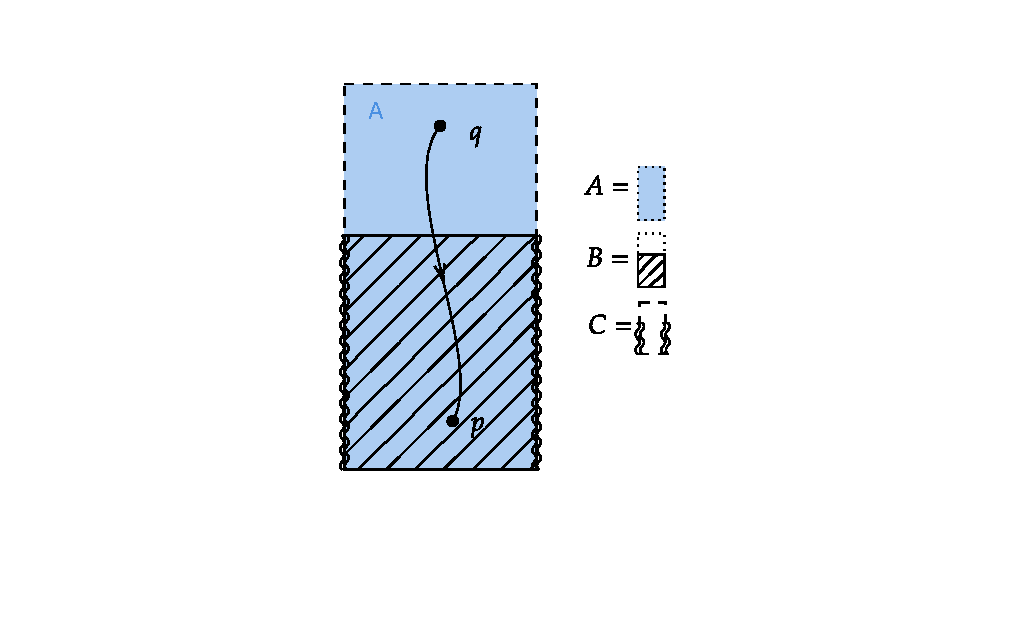
\includegraphics{Text/Pictures/general Proof idea.pdf}
	
	From the perspective of K-theory a regular index pair for a critical point is the same as a sphere with the dimension beeing the index of said critical point. To see this just use a small index pair in a Morse chart (they are all homotopic anyway), collaps the stable part and quotiend by the exit set. By doing this we get the communative diagramm:
		\begin{center}
	% https://tikzcd.yichuanshen.de/#N4Igdg9gJgpgziAXAbVABwnAlgFyxMJZABgBpiBdUkANwEMAbAVxiRAGkA9YAawFoAjAF8AFACFSAYQCUIIaXSZc+QigHkqtRizZdeogIKkxs+Yux4CRMgM31mrRB279hIgMovBQ0wpAYLFSJ1W2p7HSc9HlFPXm9fc2UrFDIAJjttR2d9DxcfOU0YKABzeCJQADMAJwgAWyQyEBwIJFSzEGq6pHUmlsQAZnbO+sRG5u6wzLYAHWnYBhw6AH1gHCqsNAYYITk-YdbqcYGhmpGAFkO+wb3Tg96kM6EKISA
	\begin{tikzcd}
		{K^{k-1}(B,C)} \arrow[d] \arrow[r, "\delta_{triple}"] & {K^{k}(A,B)} \arrow[d] \\
		K^{k-1}(S^{k-1}) \arrow[r] \arrow[d]                  & K^{k}(S^{k-1})         \\
		K^{k}(S^{k}) \arrow[ru]                               &                       
	\end{tikzcd}
		\end{center} And as a map between K Groups of spheres, we know that this map corresponds to the question of orientation. Now we have the maps 
		\begin{enumerate}[(a)]
			\item $S^k\to S\vee (B\big/ C)$ induced from an orientation in the unstable manifold arround $p$ together with $-\grad(f)(x_i)$ where $x_i\in W(q\to p)$. 
			\item $S^k \to (A\big/ B)$ induced from an orientation in the unstable manifold arround $q$. 
		\end{enumerate}
		And hence the diagram 
		\begin{center}
			% https://tikzcd.yichuanshen.de/#N4Igdg9gJgpgziAXAbVABwnAlgFyxMJZABgBpiBdUkANwEMAbAVxiRAGkA9YAawF8AFAGUAOiJowYAAgEAhUgGEAlEpB9S6TLnyEUARlJ6qtRizZdegoZx6r1m7HgJEATOWP1mrRB278BAIKksnbGMFAA5vBEoABmAE4QALZIZCA4EEhuJl5sYrAMOHQA+sA48VhoDDB8ahogCclIBumZiC72DYkpiC0ZqXwUfEA
			\begin{tikzcd}
				{K^{k}(S\vee (B,C))} \arrow[rr, "\delta_{triple}"] &                                  & {K^{k}(A,B)} \\
				& K^{k}(S^k) \arrow[ru] \arrow[lu] &             
			\end{tikzcd}
		\end{center}
		The map now factors over The K-Group of a bouquette of $k$-spheres generated over the connecting flow lines. In each such sphere the comparison of orientations happens.
\end{Iprove}

Bevore we start proving this we need the lemma: 

\begin{lemma}\label{lem: The Main Lemma Np is tubular}
We work in a compact, riemanian, orientable, smooth Manifold $(M,g)$ of dimension $m$ together with a Morse-Smale funktion 
\begin{align}
	f: M\to \R
\end{align}
We assume that $q$ is a critical point of index $k+1$ and $p$ is a critical point of index $k$. we define $f(q)=b$ and $f(p)=a$ and assume that there is no critical point in $f^{-1}(a,b)\subseteq M$. We define the sub and superlevelsets 
\begin{align}
	M^t:=\{ x\in M | f(x)\leq t \} \quad \text{and}\quad M_t:=\{ x\in M | f(x)\geq t \} \, ,
\end{align} and the constants 
\begin{align}
	c \in (a,b) \quad , \quad \epsilon >0 \text{ small } \quad,\quad T>0 \text{ big .}
\end{align} With this we define the sets: 
\begin{align}
	N_q  & \coloneq    \{ x\in M_c |f(\phi_{-T}(x))  \leq b+ \epsilon  \}   \, ,  \\
	L_q  & \coloneq    \{ x\in N_q |f(x)             =    c            \}    \, , \\
	N_p  & \coloneq    \{ x\in M^c |f(\phi_T(x))     \geq a-\epsilon   \}    \, , \\
	L_p  & \coloneq    \{ x\in N_p |f( \phi_T(x))    =    a-\epsilon   \} \, ,
\end{align} and finally: 
\begin{align}
	C  & \coloneq  N_p \cup N_q  \, ,                     \\
	B  & \coloneq  N_p \cup L_q   \, ,                   \\
	A  & \coloneq  L_p \cup \mathring{(L_q-N_p)} \, .
\end{align}

	We claim that 
	\begin{enumerate}
		\item $(N_q,L_q)$ is a regular index pair for $q$\, . \label{lem: enum: 1}
		\item $(C,B)$ is an index pair for $q$\, .\label{lem: enum: 2}
		\item $(N_p,L_p)$ is a regular index pair for $p$\, .\label{lem: enum: 3}
		\item $(B,A)$ is an index pair for $p$\, .\label{lem: enum: 4}
		\item $N_p$ is a tubular neighbourhood of $W(\to p)\cap M^c$.\label{lem: enum: 5}
	\end{enumerate}
\end{lemma}

The statements \ref{lem: enum: 1}-\ref{lem: enum: 4} are easy to proof by the definitions. The regularity can be derived from a general fact for pairs $(X,Y)$ in metric spaces: If $Y$ is closed in $X$ and there is a neighbourhood of $Y$ that is open in $X$ such that $Y$ is a strong deformation retract of $U$. So the only thing left to show is, that $N_p$ is a tubular neighbourhood. in \cite{MorseTheorySalmbon} in the proof of lemma 3.2 Salamon claims this to be true without a proof (page 119 in the attached source). Similar, in \cite{banyaga2004lectures} Banyaga claims this (also without any argument).
I find this difficult to proof, since we cannot use the flow for the map from the normal bundle, as points leave $N_p$ along the flow: The Set $N_p$ is sketched in the figure below. 
\begin{center}
	
	
	\tikzset{every picture/.style={line width=0.75pt}} %set default line width to 0.75pt        
	\resizebox{\linewidth}{!}{%
		
		
		
		\tikzset{every picture/.style={line width=0.75pt}} %set default line width to 0.75pt      
		
		\tikzset{every picture/.style={line width=0.75pt}} %set default line width to 0.75pt        
		
		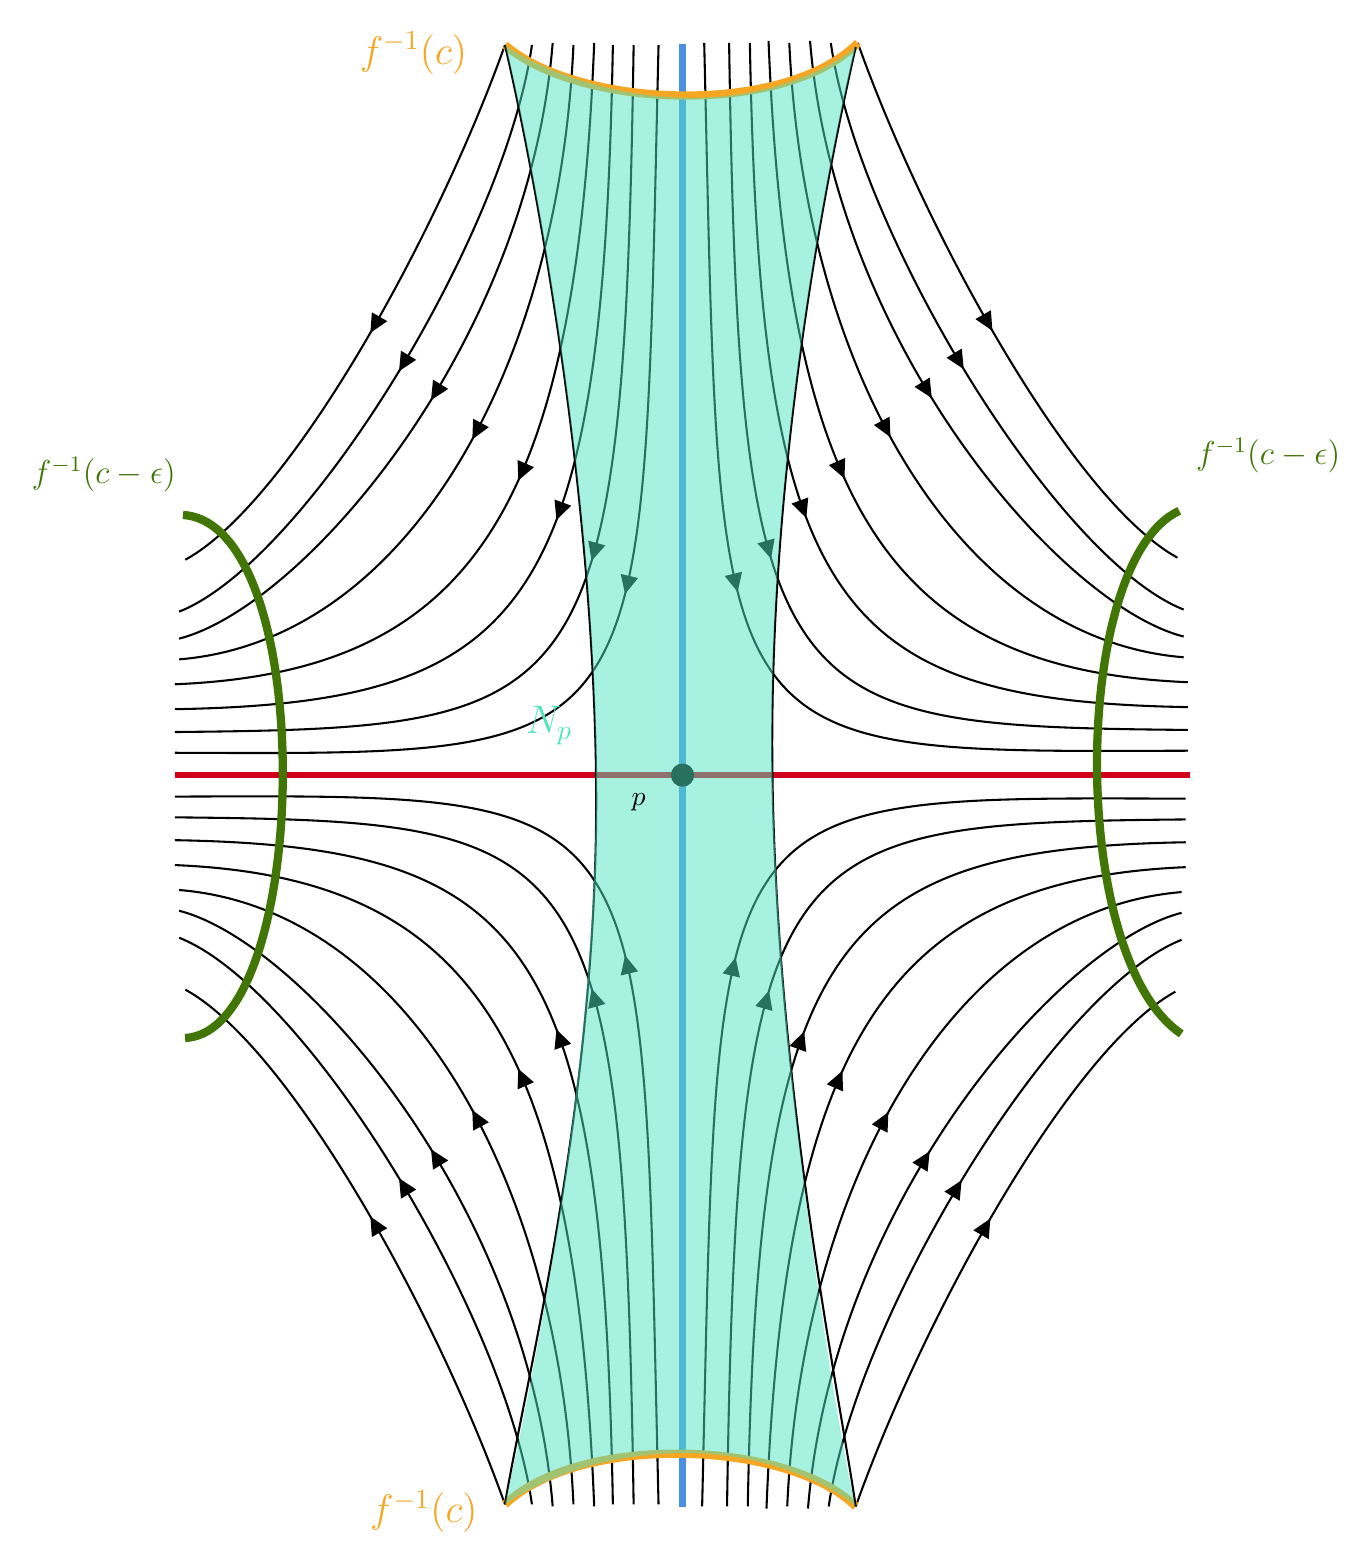
\begin{tikzpicture}[x=0.75pt,y=0.75pt,yscale=-1,xscale=1]
			%uncomment if require: \path (0,843); %set diagram left start at 0, and has height of 843
			
			%Straight Lines [id:da11875089429305197] 
			\draw [color={rgb, 255:red, 74; green, 144; blue, 226 }  ,draw opacity=1 ][line width=2.25]    (329,31.6) -- (329,736.43) ;
			%Straight Lines [id:da5325201497809933] 
			\draw [color={rgb, 255:red, 208; green, 2; blue, 27 }  ,draw opacity=1 ][line width=2.25]    (84.42,384.02) -- (573.58,384.02) ;
			%Shape: Circle [id:dp07579894054308489] 
			\draw  [draw opacity=0][fill={rgb, 255:red, 0; green, 0; blue, 0 }  ,fill opacity=1 ] (323.4,384.02) .. controls (323.4,380.92) and (325.91,378.42) .. (329,378.42) .. controls (332.09,378.42) and (334.6,380.92) .. (334.6,384.02) .. controls (334.6,387.11) and (332.09,389.62) .. (329,389.62) .. controls (325.91,389.62) and (323.4,387.11) .. (323.4,384.02) -- cycle ;
			%Curve Lines [id:da1665503577346341] 
			\draw    (339.45,31.25) .. controls (347.8,378.2) and (336.45,373.05) .. (572.45,372.25) ;
			\draw [shift={(355.57,295.75)}, rotate = 256.55] [fill={rgb, 255:red, 0; green, 0; blue, 0 }  ][line width=0.08]  [draw opacity=0] (8.93,-4.29) -- (0,0) -- (8.93,4.29) -- cycle    ;
			%Curve Lines [id:da7994448259938868] 
			\draw    (351.45,31.25) .. controls (356.45,355.25) and (373.45,360.25) .. (572.45,362.25) ;
			\draw [shift={(371.68,279.76)}, rotate = 253.92] [fill={rgb, 255:red, 0; green, 0; blue, 0 }  ][line width=0.08]  [draw opacity=0] (8.93,-4.29) -- (0,0) -- (8.93,4.29) -- cycle    ;
			%Curve Lines [id:da558792425961241] 
			\draw    (361.45,31.25) .. controls (366.45,302.25) and (401.45,348.25) .. (572.45,351.25) ;
			\draw [shift={(388.63,260.1)}, rotate = 249.87] [fill={rgb, 255:red, 0; green, 0; blue, 0 }  ][line width=0.08]  [draw opacity=0] (8.93,-4.29) -- (0,0) -- (8.93,4.29) -- cycle    ;
			%Curve Lines [id:da5211576581151481] 
			\draw    (370.45,30.25) .. controls (379.45,254.25) and (428.45,333.25) .. (572.45,339.25) ;
			\draw [shift={(407.03,241.09)}, rotate = 246.23] [fill={rgb, 255:red, 0; green, 0; blue, 0 }  ][line width=0.08]  [draw opacity=0] (8.93,-4.29) -- (0,0) -- (8.93,4.29) -- cycle    ;
			%Curve Lines [id:da39021575553782684] 
			\draw    (380.45,31.25) .. controls (387.45,187.25) and (460.45,318.25) .. (570.45,327.25) ;
			\draw [shift={(429.18,221.22)}, rotate = 242] [fill={rgb, 255:red, 0; green, 0; blue, 0 }  ][line width=0.08]  [draw opacity=0] (8.93,-4.29) -- (0,0) -- (8.93,4.29) -- cycle    ;
			%Curve Lines [id:da6126506516051217] 
			\draw    (390.45,30.25) .. controls (402.45,177.25) and (511.45,302.25) .. (570.45,317.25) ;
			\draw [shift={(449.07,202.35)}, rotate = 238.74] [fill={rgb, 255:red, 0; green, 0; blue, 0 }  ][line width=0.08]  [draw opacity=0] (8.93,-4.29) -- (0,0) -- (8.93,4.29) -- cycle    ;
			%Curve Lines [id:da24082042581971141] 
			\draw    (400.45,31.25) .. controls (413.45,123.25) and (509.45,280.25) .. (570.45,304.25) ;
			\draw [shift={(464.47,188.39)}, rotate = 239.04] [fill={rgb, 255:red, 0; green, 0; blue, 0 }  ][line width=0.08]  [draw opacity=0] (8.93,-4.29) -- (0,0) -- (8.93,4.29) -- cycle    ;
			%Curve Lines [id:da5298362087143788] 
			\draw    (413.45,31.25) .. controls (445.45,121.25) and (516.45,251.25) .. (567.45,279.25) ;
			\draw [shift={(478.29,169.92)}, rotate = 240.15] [fill={rgb, 255:red, 0; green, 0; blue, 0 }  ][line width=0.08]  [draw opacity=0] (8.93,-4.29) -- (0,0) -- (8.93,4.29) -- cycle    ;
			
			%Curve Lines [id:da21918221686589523] 
			\draw    (317.45,32.25) .. controls (309.1,379.2) and (320.45,374.05) .. (84.45,373.25) ;
			\draw [shift={(301.33,296.75)}, rotate = 283.45] [fill={rgb, 255:red, 0; green, 0; blue, 0 }  ][line width=0.08]  [draw opacity=0] (8.93,-4.29) -- (0,0) -- (8.93,4.29) -- cycle    ;
			%Curve Lines [id:da34745008178206616] 
			\draw    (305.45,32.25) .. controls (300.45,356.25) and (283.45,361.25) .. (84.45,363.25) ;
			\draw [shift={(285.22,280.76)}, rotate = 286.08] [fill={rgb, 255:red, 0; green, 0; blue, 0 }  ][line width=0.08]  [draw opacity=0] (8.93,-4.29) -- (0,0) -- (8.93,4.29) -- cycle    ;
			%Curve Lines [id:da8640093846313118] 
			\draw    (295.45,32.25) .. controls (290.45,303.25) and (255.45,349.25) .. (84.45,352.25) ;
			\draw [shift={(268.27,261.1)}, rotate = 290.13] [fill={rgb, 255:red, 0; green, 0; blue, 0 }  ][line width=0.08]  [draw opacity=0] (8.93,-4.29) -- (0,0) -- (8.93,4.29) -- cycle    ;
			%Curve Lines [id:da925990106139973] 
			\draw    (286.45,31.25) .. controls (277.45,255.25) and (228.45,334.25) .. (84.45,340.25) ;
			\draw [shift={(249.87,242.09)}, rotate = 293.77] [fill={rgb, 255:red, 0; green, 0; blue, 0 }  ][line width=0.08]  [draw opacity=0] (8.93,-4.29) -- (0,0) -- (8.93,4.29) -- cycle    ;
			%Curve Lines [id:da08743123557319321] 
			\draw    (276.45,32.25) .. controls (269.45,188.25) and (196.45,319.25) .. (86.45,328.25) ;
			\draw [shift={(227.72,222.22)}, rotate = 298] [fill={rgb, 255:red, 0; green, 0; blue, 0 }  ][line width=0.08]  [draw opacity=0] (8.93,-4.29) -- (0,0) -- (8.93,4.29) -- cycle    ;
			%Curve Lines [id:da08430775562121551] 
			\draw    (266.45,31.25) .. controls (254.45,178.25) and (145.45,303.25) .. (86.45,318.25) ;
			\draw [shift={(207.83,203.35)}, rotate = 301.26] [fill={rgb, 255:red, 0; green, 0; blue, 0 }  ][line width=0.08]  [draw opacity=0] (8.93,-4.29) -- (0,0) -- (8.93,4.29) -- cycle    ;
			%Curve Lines [id:da38820398572752524] 
			\draw    (256.45,32.25) .. controls (243.45,124.25) and (147.45,281.25) .. (86.45,305.25) ;
			\draw [shift={(192.43,189.39)}, rotate = 300.96] [fill={rgb, 255:red, 0; green, 0; blue, 0 }  ][line width=0.08]  [draw opacity=0] (8.93,-4.29) -- (0,0) -- (8.93,4.29) -- cycle    ;
			%Curve Lines [id:da5677669307058717] 
			\draw    (243.45,32.25) .. controls (211.45,122.25) and (140.45,252.25) .. (89.45,280.25) ;
			\draw [shift={(178.61,170.92)}, rotate = 299.85] [fill={rgb, 255:red, 0; green, 0; blue, 0 }  ][line width=0.08]  [draw opacity=0] (8.93,-4.29) -- (0,0) -- (8.93,4.29) -- cycle    ;
			
			%Curve Lines [id:da5375642083324416] 
			\draw    (338.45,736.36) .. controls (346.8,389.41) and (335.45,394.56) .. (571.45,395.36) ;
			\draw [shift={(354.57,471.87)}, rotate = 103.45] [fill={rgb, 255:red, 0; green, 0; blue, 0 }  ][line width=0.08]  [draw opacity=0] (8.93,-4.29) -- (0,0) -- (8.93,4.29) -- cycle    ;
			%Curve Lines [id:da5126738644229648] 
			\draw    (350.45,736.36) .. controls (355.45,412.36) and (372.45,407.36) .. (571.45,405.36) ;
			\draw [shift={(370.68,487.86)}, rotate = 106.08] [fill={rgb, 255:red, 0; green, 0; blue, 0 }  ][line width=0.08]  [draw opacity=0] (8.93,-4.29) -- (0,0) -- (8.93,4.29) -- cycle    ;
			%Curve Lines [id:da5839119584885231] 
			\draw    (360.45,736.36) .. controls (365.45,465.36) and (400.45,419.36) .. (571.45,416.36) ;
			\draw [shift={(387.63,507.52)}, rotate = 110.13] [fill={rgb, 255:red, 0; green, 0; blue, 0 }  ][line width=0.08]  [draw opacity=0] (8.93,-4.29) -- (0,0) -- (8.93,4.29) -- cycle    ;
			%Curve Lines [id:da975815253328843] 
			\draw    (369.45,737.36) .. controls (378.45,513.36) and (427.45,434.36) .. (571.45,428.36) ;
			\draw [shift={(406.03,526.52)}, rotate = 113.77] [fill={rgb, 255:red, 0; green, 0; blue, 0 }  ][line width=0.08]  [draw opacity=0] (8.93,-4.29) -- (0,0) -- (8.93,4.29) -- cycle    ;
			%Curve Lines [id:da9314613290760876] 
			\draw    (379.45,736.36) .. controls (386.45,580.36) and (459.45,449.36) .. (569.45,440.36) ;
			\draw [shift={(428.18,546.4)}, rotate = 118] [fill={rgb, 255:red, 0; green, 0; blue, 0 }  ][line width=0.08]  [draw opacity=0] (8.93,-4.29) -- (0,0) -- (8.93,4.29) -- cycle    ;
			%Curve Lines [id:da09174306781681929] 
			\draw    (389.45,737.36) .. controls (401.45,590.36) and (510.45,465.36) .. (569.45,450.36) ;
			\draw [shift={(448.07,565.26)}, rotate = 121.26] [fill={rgb, 255:red, 0; green, 0; blue, 0 }  ][line width=0.08]  [draw opacity=0] (8.93,-4.29) -- (0,0) -- (8.93,4.29) -- cycle    ;
			%Curve Lines [id:da21494064860512774] 
			\draw    (399.45,736.36) .. controls (412.45,644.36) and (508.45,487.36) .. (569.45,463.36) ;
			\draw [shift={(463.47,579.22)}, rotate = 120.96] [fill={rgb, 255:red, 0; green, 0; blue, 0 }  ][line width=0.08]  [draw opacity=0] (8.93,-4.29) -- (0,0) -- (8.93,4.29) -- cycle    ;
			%Curve Lines [id:da506519829239\end{proo7652] 
				\draw    (412.45,736.36) .. controls (444.45,646.36) and (515.45,516.36) .. (566.45,488.36) ;
				\draw [shift={(477.29,597.7)}, rotate = 119.85] [fill={rgb, 255:red, 0; green, 0; blue, 0 }  ][line width=0.08]  [draw opacity=0] (8.93,-4.29) -- (0,0) -- (8.93,4.29) -- cycle    ;
				
				%Curve Lines [id:da3880154567702636] 
				\draw    (317.45,735.36) .. controls (309.1,388.41) and (320.45,393.56) .. (84.45,394.36) ;
				\draw [shift={(301.33,470.87)}, rotate = 76.55] [fill={rgb, 255:red, 0; green, 0; blue, 0 }  ][line width=0.08]  [draw opacity=0] (8.93,-4.29) -- (0,0) -- (8.93,4.29) -- cycle    ;
				%Curve Lines [id:da9327211409936709] 
				\draw    (305.45,735.36) .. controls (300.45,411.36) and (283.45,406.36) .. (84.45,404.36) ;
				\draw [shift={(285.22,486.86)}, rotate = 73.92] [fill={rgb, 255:red, 0; green, 0; blue, 0 }  ][line width=0.08]  [draw opacity=0] (8.93,-4.29) -- (0,0) -- (8.93,4.29) -- cycle    ;
				%Curve Lines [id:da09647590503157577] 
				\draw    (295.45,735.36) .. controls (290.45,464.36) and (255.45,418.36) .. (84.45,415.36) ;
				\draw [shift={(268.27,506.52)}, rotate = 69.87] [fill={rgb, 255:red, 0; green, 0; blue, 0 }  ][line width=0.08]  [draw opacity=0] (8.93,-4.29) -- (0,0) -- (8.93,4.29) -- cycle    ;
				%Curve Lines [id:da15668737739736305] 
				\draw    (286.45,736.36) .. controls (277.45,512.36) and (228.45,433.36) .. (84.45,427.36) ;
				\draw [shift={(249.87,525.52)}, rotate = 66.23] [fill={rgb, 255:red, 0; green, 0; blue, 0 }  ][line width=0.08]  [draw opacity=0] (8.93,-4.29) -- (0,0) -- (8.93,4.29) -- cycle    ;
				%Curve Lines [id:da5883237308999977] 
				\draw    (276.45,735.36) .. controls (269.45,579.36) and (196.45,448.36) .. (86.45,439.36) ;
				\draw [shift={(227.72,545.4)}, rotate = 62] [fill={rgb, 255:red, 0; green, 0; blue, 0 }  ][line width=0.08]  [draw opacity=0] (8.93,-4.29) -- (0,0) -- (8.93,4.29) -- cycle    ;
				%Curve Lines [id:da9204033290837756] 
				\draw    (266.45,736.36) .. controls (254.45,589.36) and (145.45,464.36) .. (86.45,449.36) ;
				\draw [shift={(207.83,564.26)}, rotate = 58.74] [fill={rgb, 255:red, 0; green, 0; blue, 0 }  ][line width=0.08]  [draw opacity=0] (8.93,-4.29) -- (0,0) -- (8.93,4.29) -- cycle    ;
				%Curve Lines [id:da49739155745577546] 
				\draw    (256.45,735.36) .. controls (243.45,643.36) and (147.45,486.36) .. (86.45,462.36) ;
				\draw [shift={(192.43,578.22)}, rotate = 59.04] [fill={rgb, 255:red, 0; green, 0; blue, 0 }  ][line width=0.08]  [draw opacity=0] (8.93,-4.29) -- (0,0) -- (8.93,4.29) -- cycle    ;
				%Curve Lines [id:da32213499249738287] 
				\draw    (243.45,735.36) .. controls (211.45,645.36) and (140.45,515.36) .. (89.45,487.36) ;
				\draw [shift={(178.61,596.7)}, rotate = 60.15] [fill={rgb, 255:red, 0; green, 0; blue, 0 }  ][line width=0.08]  [draw opacity=0] (8.93,-4.29) -- (0,0) -- (8.93,4.29) -- cycle    ;
				
				
				%Curve Lines [id:da05541171078629925] 
				\draw [color={rgb, 255:red, 245; green, 166; blue, 35 }  ,draw opacity=1 ][line width=3]    (243.45,32.25) .. controls (279.42,63.08) and (378.33,66.67) .. (413.45,31.25) ;
				%Curve Lines [id:da4989004892868002] 
				\draw [color={rgb, 255:red, 245; green, 166; blue, 35 }  ,draw opacity=1 ][line width=3]    (243.45,735.36) .. controls (280.33,700.67) and (380.33,704.67) .. (412.45,736.36) ;
				%Curve Lines [id:da44411839842500755] 
				\draw [color={rgb, 255:red, 65; green, 117; blue, 5 }  ,draw opacity=1 ][line width=3]    (88.33,258.67) .. controls (154.22,262.97) and (150.33,507.67) .. (89.33,510.67) ;
				%Curve Lines [id:da05367202270104565] 
				\draw [color={rgb, 255:red, 65; green, 117; blue, 5 }  ,draw opacity=1 ][line width=3]    (568.33,256.67) .. controls (516.33,280.67) and (514.33,471.67) .. (569.33,508.67) ;
				%Curve Lines [id:da7969530986481941] 
				\draw    (243.45,32.25) .. controls (254.33,78.67) and (285.1,230.49) .. (287.33,382.67) .. controls (289.57,534.85) and (253.34,675.31) .. (243.45,735.36) ;
				%Curve Lines [id:da5283140439270424] 
				\draw    (412.45,33.25) .. controls (400.33,86.67) and (370.1,232.49) .. (372.33,384.67) .. controls (374.57,536.85) and (404.33,680.67) .. (412.45,736.36) ;
				
				%Shape: Polygon Curved [id:ds3817941045439226] 
				\draw  [draw opacity=0][fill={rgb, 255:red, 80; green, 227; blue, 194 }  ,fill opacity=0.5 ] (243.45,735.36) .. controls (243.39,735.01) and (288.33,547.67) .. (287.33,382.67) .. controls (286.33,217.67) and (244.39,31.96) .. (243.45,32.25) .. controls (242.51,32.54) and (278.33,56.67) .. (330.33,57.67) .. controls (382.33,58.67) and (412.39,33.99) .. (412.45,33.25) .. controls (412.51,32.51) and (368.33,212.67) .. (372.33,384.67) .. controls (376.33,556.67) and (411.01,736.21) .. (412.45,736.36) .. controls (413.89,736.52) and (381.33,709.67) .. (327.33,710.67) .. controls (273.33,711.67) and (243.51,735.72) .. (243.45,735.36) -- cycle ;
				
				% Text Node
				\draw (303,391.4) node [anchor=north west][inner sep=0.75pt]    {$p$};
				% Text Node
				\draw (172,24.4) node [anchor=north west][inner sep=0.75pt]  [font=\Large,color={rgb, 255:red, 245; green, 166; blue, 35 }  ,opacity=1 ]  {$f^{-1}( c)$};
				% Text Node
				\draw (177,727.07) node [anchor=north west][inner sep=0.75pt]  [font=\Large,color={rgb, 255:red, 245; green, 166; blue, 35 }  ,opacity=1 ]  {$f^{-1}( c)$};
				% Text Node
				\draw (14,229.4) node [anchor=north west][inner sep=0.75pt]  [font=\large,color={rgb, 255:red, 65; green, 117; blue, 5 }  ,opacity=1 ]  {$f^{-1}( c-\epsilon )$};
				% Text Node
				\draw (575,220.4) node [anchor=north west][inner sep=0.75pt]  [font=\large,color={rgb, 255:red, 65; green, 117; blue, 5 }  ,opacity=1 ]  {$f^{-1}( c-\epsilon )$};
				% Text Node
				\draw (252,349.4) node [anchor=north west][inner sep=0.75pt]  [font=\Large,color={rgb, 255:red, 80; green, 227; blue, 194 }  ,opacity=1 ]  {$N_{p}$};
				
				
			\end{tikzpicture}
			
			
		}
	\end{center}
	So to proof this, we first formulate two lemmas. First we restate/ refine the $\lambda$-lemma: \todo{parameter dependence einfügen}
	\begin{lemma}[The Technical $\lambda-$Lemma] 
		Let $ M$ be a smooth manifold and let $p$ be a hyperbolic fixpoint of a diffeomorphism $\phi$ on $M$ with $\dim W(p \to)=r$ for ${0<r<m=\dim M}$. Let $N$ be an injective immersed submanifold of $M$ that is invariant under $\phi$ and has a point of transverse intersection $q$ with $W(\to p)$. Then for any $\epsilon>0$, any $r-$cell neighbourhood $D$ of $q$ in $N$ that also intersects $W(\to p)$ transversal and any $r-cell$ neighbourhood $B$ of $p$ in $W(p\to))$ there is a smaller cell $\tilde{D}\subset D$, an $n\in \N$ such that the following is true:
		
		We can assume that $B$ and $\phi^n(\tilde{D})$ lives in a chart centered at $p$ with a product structure $U\cong W(\to p)\cap B_\mu(0)\times W(p\to)\cap B_\mu(0)$. Here,the invers of the projection into $B\subseteq W(\to p)$:
		\begin{equation*}
			h: B\to \phi^n(\tilde{D})\, 
		\end{equation*}satisfies:
		\begin{enumerate}
			\item $\sup_{x \in B}\norm{x-h(x)}<\epsilon$ and
			\item For the inclusions  $i_1:B\to M$ and $i_2:\phi^n(\tilde{D})\to M$ we have that 
			\begin{equation*}
				\sup_{x \in B}\norm{\diff(i_1)_x-\diff(i_2\circ h)_x}<\epsilon\, .
			\end{equation*}
		\end{enumerate}
	\end{lemma}
	\begin{proof}
		\begin{comment}
		Let \( q \) be a point of transversal intersection of \( W(\to p) \) with \( N \). Since both \( N \) and \( W(\to p) \) are invariant under \( \phi \), it follows that \( \phi^n(q) \in N \cap W(\to p) \) for all \( n \in \N \). Moreover, the intersection remains transversal: the direct sum decomposition \( T_q M = T_q W(\to p) \oplus T_q N \) is preserved under \( d\phi_q \), which implies transversality at \( \phi^n(q) \) as well.
		
		Therefore, we may assume that \( q \) lies in a coordinate chart centered at the hyperbolic fixed point \( p \), and identify a neighborhood of \( p \) with an open subset of \( \mathbb{R}^m \), where \( m = \dim M \). By hyperbolicity of \( p \), the tangent space at \( p \) splits as
		\[
		T_p M = T^s_p M \oplus T^u_p M,
		\]
		and this splitting is preserved by \( d\phi_p \). As discussed earlier\todo{reference einfügen}, there exists a chart in which \( d\phi_p \) is represented by a real diagonal matrix (in suitable coordinates)\todo{in fact we can choose a Morse chart that satisfies this!}. Hence, we may choose an orthonormal basis of coordinates \( (x_s, x_u) \in \mathbb{R}^s \times \mathbb{R}^u \), adapted to the stable and unstable subspaces, such that
		\[
		d\phi_0 =
		\begin{pmatrix}
			A & 0 \\
			0 & B
		\end{pmatrix},
		\]
		where the eigenvalues of \( A \) have modulus less than 1, and those of \( B \) greater than 1.
		
		Since we are working in \( \mathbb{R}^m \), we identify the manifold and its tangent space locally around 0. We then expand \( \phi \) in a Taylor series at the origin:
		\[
		\phi(x_s, x_u) = \phi(0) + d\phi_0(x_s, x_u) + f(x_s, x_u),
		\]
		where \( f(0) = 0 \) and \( df(0) = 0 \). Writing this in coordinates gives:
		\begin{equation} \label{eq: proof of Lambda lemma phi split}
			\phi(x_s, x_u) = (A x_s + f_s(x_s, x_u),\; B x_u + f_u(x_s, x_u)).
		\end{equation}
		Furthermore, since $f=\phi-\diff \phi|_0$ we know that: 
		\begin{align*}
			\frac{\partial f_s}{\partial x_u}|_{(0,x_u)}=\frac{\partial \phi_s}{\partial x_u}|_{(0,x_u)}=0=\frac{\partial f_u}{\partial x_s}|_{(x_s,0)}=\frac{\partial \phi_u}{\partial x_s}|_{(x_s,0)}.
		\end{align*} Similar to Corollary $\ref{cor: Tangendspace splits}$ we can define an inner product such that for the operator norm we have 
		\begin{align*}
			\norm{A}\leq \alpha <1 \quad \text{ and } \quad \norm{B^{-1}}\leq \frac{1}{\beta} <1.
		\end{align*}
		Since $1=\norm{\id}=\norm{BB^{-1}}\leq \norm{B}\cdot \norm{B^{-1}}$ we know that $\norm{B}\geq \beta$.
		For a neighbourhood $U_1\subseteq U$ of the origin we define 
		\begin{align*}
			k:=\max_{i,j=s,u} \Bigg\{ \sup_{\overline{U_1}}\norm{\frac{\partial f_i}{\partial x_j}} \Bigg\},
		\end{align*} and choose $U_1$ small enough such that $k$ satisfies:
		
		
		\begin{gather*}
			0<k<1 \\
			\beta_1:=\beta -k >1 \\
			\alpha_1:=\alpha +k <1 \\
			k<\frac{1}{4}(b_1-1)^2.
		\end{gather*}
		This can be achieved since $\diff f\big|_0=0$.
		Let $B$ be a cell neighbourhood of the origin in $W(p\to )$. For some $n \in \N$ we have that $\phi^{-n}(B)\subseteq U_1$. If the $\lambda-$lemma holds for $\phi^{-n}(B)$ for all $\epsilon$ it also holds for $B$, since the metric and $\phi$ are continuous and the $r-$cell is compact. Therefore, the change of distance after applying $\phi^{-n}$ is finite and we can choose the distance from $\phi^{-n}(B)$ to $D$ small enough such that $B$ is $\epsilon~C^1$-close to $D$. Hence, without restrictions $B\subseteq U_1$ and $q\in U_1$.  Next we define the inclination of $N$ with respect to the (un-)stable manifolds as follows: 
		
		Let $x\subseteq N \cap U_1$ and $v^0\in T_xN\subseteq T_0M=T^s_0M \oplus T^u_oM$ and let $v^0=(v_s^0,v_u^0)$ be the coordinate entries. Furthermore let $v$ be a unit vector. Now we define the \textbf{inclination} of $v^0$:
		\begin{align*}
			\lambda(v^0)=\frac{\norm{v^0_s}}{\norm{v^0_u}}.
		\end{align*}
		In other words: The smaller the inclination, the more parallel we are to $W(p\to)$. Notive how we can only define the inclination if $v^0_u\neq 0$. 
		Furthermore define:
		\begin{align*} x^n:=\phi^n(x), ~v^n:= \diff \phi_{x^{n-1}}(v^{n-1}) \text{ and } \phi(x)=(\phi_s(x),\phi_u(x))\in W(\to 0)\times W(0\to).
		\end{align*}
		Now we want to calculate the derivative $\diff \phi|_{q^n}$. But first inspect:
		\begin{align*}
			\diff \phi|_x=\begin{pmatrix}
				\frac{\partial \phi_s}{\partial x_s}|_{x} & \frac{\partial \phi_s}{\partial x_u} |_{x}\\
				\frac{\partial \phi_u}{\partial x_s} |_{x}& \frac{\partial \phi_u}{\partial x_u}|_{x}
			\end{pmatrix}\overset{(\ref{eq: proof of Lambda lemma phi split}) }{~=~}
			\begin{pmatrix}
				A+ \frac{\partial f_s}{\partial x_s}|_{x}& \frac{\partial f_s}{\partial x_u}|_{x}\\
				\frac{\partial f_u}{\partial x_s} |_{x} & B+ \frac{\partial f_u}{\partial x_u}|_{x}
			\end{pmatrix} 
		\end{align*} Since $q^n\in W(\to 0)$ and $\frac{\partial f_u}{\partial x_s}(x_s,u)$=0 this gives us:
		
		\begin{align*}
			\diff \phi|_{q^n}=\begin{pmatrix}
				A+ \frac{\partial f_s}{\partial x_s}|_{q^n}&    \frac{\partial f_s}{\partial x_u}|_{q^n}\\
				0                                   & B+ \frac{\partial f_u}{\partial x_u}|_{q^n}
			\end{pmatrix} 
		\end{align*}
		Let $B_s(\delta)$ denote the ball of radius $\delta$ around the origin that lives in $W(\to p)$ and $U_2:= B_s(\delta)\times B$. Since $\frac{\partial f_s}{\partial x_u}|_{(0,x_u)}=0$ and by the smoothness of  $\phi$, for any $\epsilon >0$ there exists a $\delta$ such that 
		\begin{align*}
			\underbrace{\sup_{U_2}\norm{\frac{\partial f_s}{\partial x_u}}}_{:=k_1}< \min\{\epsilon, k \}.
		\end{align*} 
		Again, we assume $q\in D\subseteq  U_2$. Now we want to get a hold of the inclination:  Let $x\in N$ such that $x^j\in U_2 $ for all $j\leq n$ and let $v^0\in T_xN$. Denote $v^n=(v^n_s,v^n_u)\in T_0W(\to 0)\times T_0W(0 \to)$. 
		\begin{align}
			\lambda(v^n)&= \frac{\norm{\diff \phi_s|_{x^{n-1}}(v^{n-1})}}{\norm{\diff \phi_u|_{x^{n-1}}(v^{n-1})}} \nonumber \\
			&=\frac{\norm{Av_s^{n-1} +\ \frac{\partial f_s}{\partial x_s}|_{x^{n-1}}v_s^{n-1} \ \, + \, \frac{\partial f_s}{\partial x_u}|_{x^{n-1}}(v_u^{n-1})}}{\norm{\color{blue} \frac{\partial f_u}{\partial x_s}|_{x^{n-1}}(v_s^{n-1}) \color{black}+   Bv_u^{n-1}+\frac{\partial f_u}{\partial x_u}|_{x^{n-1}}(v_u^{n-1})}} \nonumber \\
			& \leq \frac{ (\alpha +k )\norm{v_s^{n-1}}+k_1 \norm{(v_u^{n-1})}}
			{ \color{blue}k \norm{(v_s^{n-1})} \color{black}  +  (\beta+k)\norm{ v_u^{n-1}}} \nonumber \\
			& \leq \frac{ (\alpha +k )\norm{v_s^{n-1}}+k_1 \norm{(v_u^{n-1})}}
			{ (\beta-k)\norm{ v_u^{n-1}}  - \color{blue} k_1 \norm{(v_s^{n-1})} \color{black} } &\quad \text{since } \beta-k>1 \text{ and }k_1<k<1 \nonumber \\
			& = \frac{ (\alpha +k )\lambda(v^{n-1})+k_1}
			{ \beta_1  - \color{blue} k_1 \lambda{v^{n-1}\color{black} }} &\quad \text{we divided by }\norm{v_u^{n-1}} \nonumber \\
			&\leq \frac{\lambda(v^{n-1})+k_1}
			{ \beta_1  - \color{blue} k_1 \lambda(v^{n-1}) \color{black} }  \label{eq: estimate lambda(v^n)}				
		\end{align} 
		If $x\in W(\to 0)$ the blue part above disappears and we get:
		\begin{align*}
			\lambda(v^n) \leq \frac{\lambda(v^{n-1})+k_1}{\beta_1}.
		\end{align*} By induction we get:
		\begin{align}
			\lambda(v^n)\leq \frac{\lambda(v^{n-1})+k_1}{\beta_1}=\frac{\frac{\lambda(v^{n-2})+k_1}{\beta_1}+k_1}{\beta_1}= \frac{\frac{\lambda(v^{n-2})+\frac{k_1 \beta_1}{\beta_1}}{\beta_1}+k_1}{\beta_1} =\frac{\lambda(v^{n-2})+k_1+ k_1 \beta_1}{\beta_1^2}\leq \cdots \nonumber \\
			\leq \frac{\lambda(v^0)+\sum_{l=0}^{n-1}k_1 \beta_1^l}{\beta_1^n}~. \label{eq: proof lambda lemma estimate lambda(v^n) with x=q}
		\end{align} By using the geometric series we see:
		\begin{align*}
			\lambda(v^n)\leq \frac{\lambda(v^0)}{\beta_1^n}+k_1\sum_{l=1}^n\frac{1}{\beta^n} \leq \frac{\lambda(v^0)}{\beta_1^n}+k_1(\frac{1}{1-\beta_1}-1)=
			\frac{\lambda(v^0)}{\beta_1^n}+k_1(\frac{b}{\beta_1-1}-\frac{\beta_1-1}{\beta_1-1}) \\ =\frac{\lambda(v^0)}{\beta_1^n}+k_1(\frac{1}{\beta_1-1}).
		\end{align*}
		Since $\beta_1$ was greater then 1 we can conclude that $\lim_{n \to \infty}\frac{\lambda(v^0)}{\beta_1^n}=0$ and since $k<\frac{1}{4}(\beta_1-1)^2$ we know that $\frac{k}{\beta_1-1}<\frac{b-1}{4}$. Because of that, a $n_0$ exists such that for all $n>n_0$ :
		\begin{align*}
			\lambda(v^n)\leq \frac{\lambda(v^0)}{\beta_1^n}+\frac{k}{b-1}< \frac{\beta_1-1}{3}.
		\end{align*}  
		Lets collect what we have done so far: We take a point $x$ from a transverse intersection of $N$ and $W(\to p)$. Then, we inspect the inclination of a tangent vector $v$ in ${T_xN\subseteq T^s_0M\times T^u_0M}$ and move the tangent vector via $\diff \phi$ alongside of the stable set and realize that the inclination gets smaller, the more we move it. 
		
		
		
		
		
		
		For any $v\in T_{q^n}N$ there exists a $\tilde{v} \in T_qN$ such that $v=\tilde{v}^n$, since
		$\diff \phi|_x:T_xM \to T_{\phi(x)}M$ is bijective. 
		If we take an arbitrary local section $f:M \to TM$
		that denotes the choice of $v^0\in T_xN$ we know that $\lambda \circ f$ is continuous, 
		as it is the composition of continuous functions. In other words, the inclination smoothly depends on $v^0$ and $x$. 
		This tells us that for a small enough cellular neighbourhood $D_0 \subseteq D\subseteq N \cap U_2$ such that for any $x\in D_0$ and $v_0\in T_xN$ of length $1$ we have
		\begin{equation}
			\lambda(v^0)\leq \frac{1}{2} (\beta_1-1).
		\end{equation} (This is true as long as the invlination is well defined )
		Now we claim that if $\phi^j(v^0)\in U_2$ for all $j=0,...,n$ then $\lambda(v^n)\leq \frac{1}{2}(\beta_1-1).$ We prove this by induction: The case $n=0$ is already done. For the induction step we use the estimate (\ref{eq: estimate lambda(v^n)}), $k_1 <k<1$ and $k< \frac{1}{4}(\beta_1-1)^2$:
		\begin{align*}
			\lambda(v^{n+1})\leq \frac{\lambda(v^{n})+k_1}{ \beta_1  - k_1 \lambda(v^{n})}\leq \frac{ \frac{1}{2}(\beta_1-1)+\frac{1}{4}(\beta_1-1)^2}{ \beta_1  - \frac{1}{2}(\beta_1-1))} = \frac{1}{2}(\beta_1-1).
		\end{align*} Using the above estimate and (\ref{eq: estimate lambda(v^n)}) again we conclude that for all $x\in D_0$ such that $\phi^j(x)\in U_2$ for all $j=0,...,n$ and for any unit vector $v^0\in T_xN$ we have:
		\begin{align*}
			\lambda(v^{n})& \leq \frac{\lambda(v^{n-1})+k_1}{ \beta_1  - k_1 \lambda(v^{n-1})}\\
			&\leq \frac{\lambda(v^{n-1})+k_1}{ \beta_1  - \frac{1}{2}(\beta_1-1))}\\
			&\leq \frac{\lambda(v^{n-1})+k_1}{ (\frac{1}{2}(1+\beta_1))}.
		\end{align*} Notice that for $\beta_2:=\frac{1}{2}(1+\beta_1)$ we have $1<\beta_2<\beta_1$. Again like in the equation (\ref{eq: proof lambda lemma estimate lambda(v^n) with x=q}) we can use induction to conclude:
		\begin{align*}
			\lambda(v^n)\leq \frac{\lambda(v^0)}{\beta_2^n}+\frac{k_1}{\beta_2-1},
		\end{align*} and since $k_1\leq \epsilon$ we have for any $n$ large enough, any $x\in D_0$ such that $\phi^j(x) \in U_2$ for $j=0,...,n$ and any unit vector $v^0 \in T_xN$:
		\begin{align*}
			\lambda(v^b)\leq \epsilon(1+\frac{1}{\beta_2-1}).
		\end{align*}
		Let $\pi_u:U \to W(0\to)$ be the projection. Since $\phi$ is expanding on $W(0 \to)$ we know that a $n_2\geq n_1$ exists such that $B\subseteq \pi_u(D_{n_2})$, where $D_{n_2}$ denotes the connected component of $\phi^{n_2}(D_0)\cap U$ that contains $q^{n_2}$. If $\dim N > \dim W(0 \to)$ we can choose a subset of $\dim W(0\to)$ and then the projection restricted to $D_{n_2}$:  $\pi_u|{D{n_2}}$ can be modified to be one to one. For this we use the fact that we are an embedded manifold.Hence, we are given by an implicit function where the derivatives in $W(\to p)-$direction are invertible as a matrix. By the implicit function theorem we can take any point $x$ from $D_{n_2}$ and conclude that there is a neighbourhood $U(x)\subset W(p\to)$ around $\pi_u(x)$ in $D_{n_2}$ and a smooth function $G: W(p\to)\to W(\to p)$, such that around $x$ $D_{n_2}$ looks like $(y,G(y))$ telling us that the projection onto the domain of $G$ is one to one after restricting $D_{n_2}$ to $U(x)\times \im(G)$. Now we can define $h$ to be the inverse of that projection (that is $G\times \id$) and get the closeness of $B$ to $D_{n_2}$. To see that we first check the distances and the difference after differentiating. For this we need the maps: $i_1:B\to M, x \mapsto (0,x)$, and $i_2: ~D_{n^2} \to M,~ x\mapsto x$ and $h: B \to D_{n^2},~ x \mapsto \pi_u^{-1}(x)=(h_s(x),x)=(h_s(x),h_u(x)$:
		
		\begin{align*}
			\sup_{x\in B} \norm{ \diff( i_{1} )_x-\diff (i_2 \circ h )_x} &= \sup_{x\in B} \norm{ \begin{psmallmatrix}
					0 \\
					1
				\end{psmallmatrix}- \begin{psmallmatrix}
					\diff (h_s)_x \\
					1
			\end{psmallmatrix} } \\
			&=\sup _{x\in B} \norm{\diff (h_s)_x } &\\
			&= \sup_{x \in B} \sup_{\norm{v}\leq 1} \norm{\frac{\diff(h_s)_x}{\diff(h_u)_x}(v) \diff(h_u)_x}(v) & \text{ here:} \begin{cases} h_u \equiv  \id_{w(\to p)} \times h_u \\
				h_s \equiv h_s \times \id_{W(p \to)}.
			\end{cases} \\
			&=\sup_{x \in B} \sup_{\norm{v}\leq 1} \frac{\norm{(\diff(h)_x)_s(v)}}{\norm{(\diff(h)_x)_u(v)}}\norm{v}\\
			&= \sup_{x \in B} \sup_{\norm{v} = 1} \lambda(\diff h_x(v)) & \text{since $\diff h_x$ is linear} \\
			& \leq \epsilon(1+\frac{1}{\beta_2-1}).
		\end{align*} The last inequality follows from $\diff h_x(v))$ being an element in $T_xN$ and the existence of a $\tilde{v} \in D_0:\tilde{v}^n=v$. Finally since $\beta_2$ is independent of $\epsilon$ we can make this construction for any $\epsilon$.
		Furthermore since we can increase $n$ (and decrease the sice of $\tilde{D}$) such that $D_{n^2}$ is arbitrary close to the origin, the statement that 
		\begin{equation*}
			\sup_{x\in B}\norm{x-h(x)}<\epsilon 
		\end{equation*} is clear.
		
		%here stats the proof of the strukturel inclination lemma
		
		Therefore, by definition we have that for any $\mathcal{N}^r(f,(\phi,U),(\psi,V),\epsilon)$ that contains $i_2$ there is a $r-$cell $D_{n^2}$ and a $h$ such that $i_2 \circ h \in \mathcal{N}^r(f,(\phi,U),(\psi,V),\epsilon)$. This tells us that every neighbourhood of $i_1$ contains such an $h$ and therefore, in the $C^r-$generating metric $d_1$, an $r-$cell and a $h$ exists such that $d_1(i_1.i_2\circ h)<\epsilon.$ This concludes the proof of the lambda lemma.  	
		
		we proofed the same with the only difference, that we defined the $r-$cell $D$ arbitrary. We now want to show that this $r-$cell can be defined to be the image of a moved smaller cell of a given $r-cell$. So lets inspect the already given proof:
		
		We started by moving the point of transverse intersection $q$ closer to the fixpoint by applying the diffeomorphism to it. Then we defined an neighbourhood $D_0$ of that moved point in the stable manifold (compare \ref{eq: proof lambda lemma small neighbourhood}). Here we were able to get a hold of the inclination. Then we moved $D_0$ via applying the isomorphism closer to the fixed point and restricted it to the dimension of the unstable manifold. This restriction we can refine as follows: First we define $D_{n^2}$ to be the moved $D_0$. Lets say we moved $q$ $n-$times. In other words $q\in \phi^{-n}(D_{n^2})$ Then there exist a small $r-$cell neighbourhood of $q$ that lives in $D \cap \phi^{-n}(D_{n^2})$. That is because $ \phi^{-n}(D_{n^2})$ is an in $N$ open neighbourhood of $y$, hence $\phi^{-n}(D_{n^2}) \cap D$ is open in $D$. Hence we can find a ball around $y$ in $D$ that is contained in the intersection. We call that $r-$cell $\tilde{D}$. Then $\phi^n(\tilde{D})$ is an $r-$dimensional subset of $D_{n^2}$ and the rest of the proof can be done with that subset. All arguments work, as that subset is transverse to $W(\to p)$. 
	\end{comment}
	The proov is essentially the same as given in David Hurtubise - Lectures on Morse Homology. I omitted it here. 
	\end{proof}
	Next we proove that fiberwise the flow is monotonly decreasing in any normal-direction with respect to $W(\to p)$:
	\begin{lemma}\label{lem: fibrewise monotopnically}
		Let $U$ be a tubular neighbourhood of $W(\to p)\cap M^c$, with $J:NW(\to p)\cap M^c\to M$ beeing the corresponding embedding. For $x\in W(\to p)\cap M^c$ we denote $U_x$ the embedded fiber over $x$. Then there exists a $T>0$ big enough and a global trivialization $\Phi: NW(\to p)\cap M^c\to  \left(W(\to p)\cap M^c\right)\times \R^{\lambda_p}$ such that the the composition $f\circ \phi_T \circ J\circ \Phi^{-1}$ is fibrewise monotonically decreasing meaning that for any  $0\neq v\in U_x$  and $\nu >0 $ small the function
		\begin{align*}
			l_v: (1-\nu,1+\nu) &\to \R\\
			\lambda &\mapsto f\circ \phi_T \circ J\circ \Phi^{-1}(x,\lambda \cdot v)
		\end{align*} has negative derivative.
	\end{lemma}
	\begin{proof}
		We will apply the technichal $\lambda$-lemma. For this we reuse the notation as follows. The lemma tells us, that for any $\mu_T>0$ we can find a $T$ big enough, such that $\phi_T(J(U_x))$ is close in the following sense: There is a neighbourhood $L$ of $p$ and a Morse chart 
		\begin{align*}
			\Psi: L\to \R^{\lambda_p}\times \R^{m-\lambda_p}
		\end{align*} such that $\restr{\Psi}{\R^{\lambda_p}}\supseteq W(p\to)$. In this chart the set $\phi_T(J(U_x))$ is the graph of a funktion $h^s_x:\R^{\lambda_p}\to \R^{m-\lambda_p}$ that satisfies:
		\begin{align*}
			\norm{\diff h^s_v}<\mu_T\\ 
			\norm{ h^s_v}<\mu_T
		\end{align*}
		We define the map $h_x=h^s_x\oplus \id_{\lambda_p}: \R^{\lambda_p}\to \R^m$.
		
		
		
		
		
		Now $\phi_T(J(U_x))=\Gamma(h^s_x)=\im (h_x)$. Using this we define our global trivialisation:
		\begin{align*}
			\Phi: NW(\to p)\cap M^c &\to  \left(W(\to p)\cap M^c\right)\times \R^{\lambda_p}\\
			\xi &\mapsto \left(\pi(\xi), h^{-1}_{\pi(\xi)}\circ \Psi \circ \phi_T \circ J(\xi)\right)
		\end{align*}
		In this trivialization the funktion $l_v$ looks like:
		\begin{align*}
			l_v(\lambda)
			&=f \circ \phi_T\circ J \circ \Phi^{-1} (x,\lambda v)\\
			&=f \circ \phi_T\circ J\circ J^{-1}\circ \phi_{-T}\circ \Psi^{-1} \circ h_x\\
			&=f \circ \Psi^{-1} \circ h_x\, .
		\end{align*} 
		In coordinates this reads:
		
		
		
		Now we can calculate its derivative to conclude the statement: 
		\begin{align*}
			\diff (l_v)(\lambda)
			&=\restr{\diff (f\circ \psi^{-1})}{h_x(\lambda v)}\circ \restr{\diff h_x}{\lambda v} (v)\\
			&=\restr{\diff (f\circ \psi^{-1})}{h_x(\lambda v)} (v,\diff h_x^s(v))\\
			&=-2\lambda \sum_{i_1}^{\lambda_p}(v^i)^2+\left(h^s_x(\lambda v)\right)^T\cdot (\diff h_x^s)^i(\lambda v)\\
			&\leq-2\lambda \norm{v}^2 +\lambda^2 (\mu^T )^2\norm{v}^2\\
			&= \left( -2+(\mu^T)^2\lambda \right) \lambda \norm{v}^2<0 \text{ for all $v\neq 0$, $\lambda \in I$ and for all $T$ big enough.}
		\end{align*}		
	\end{proof}
	Hence, the sets $N_p\cap U_x$ are starshaped with respect to the embedding of the normal space.
	
	Now we want to \textbf{smoothly} rescale to the starshaped neighbourhood. This is in general not possible and homeomorphisms from starshaped neighbourhoods to $R^n$ are hard to describe, even if they are not required to be a resacling. The main problem in the general case is, that the following: for each $v\in \phi_T(J(U_x))$ by the star shaped property there is a unique $\lambda_v$ ,  such that $f\circ (\lambda_v v)=a-\epsilon$. But the map $v\mapsto \lambda_v$ needs not to be continouos in the general starshaped setting however here it is and it even continouosly depends on $x$:
	\begin{definition}[Hyperspherical coordinates]
		For our next proof we need to introduces spherical coordinates on $R^{\lambda_{p}}$. Define $s_k\coloneq \sin(\theta_k)$ and $c_k\coloneq \cos(\theta_k)$:
		\begin{align*}
			\Lambda: \R_{\geq 0}\times [0,\pi]^{\lambda_{p}-2}\times [0,2\pi)&\to \R^{\lambda_p}  \\
			(r,\theta_1,\dots, \theta_{\lambda_p-1})&\mapsto \begin{pmatrix}
				rc_1\\
				rs_1c_2\\
				\vdots  \\
				rs_1 \cdots s_{\lambda_{p}-2} c_{\lambda_{p}-1} \\
				rs_1 \cdots s_{\lambda_{p}-2} s_{\lambda_{p}-1}		
			\end{pmatrix}
		\end{align*}
		With differential 
		\begin{align*}
			\begin{pmatrix} 
				c_1                        &-rs_1              &0        &0 &\cdots &0      \\
				s_1c_2                     &rc_1c_2            &-rs_1s_2 &0 &\cdots &0      \\
				\vdots                     &\vdots             & \vdots  &  &\ddots &\vdots \\
				&                   &         &  &             \\
				s_1\cdots s_{n-2}c_{n-1}   &\cdots             &\cdots   &  &       &-rs_1\cdots s_{n-2}s_{n-1} \\
				s_{1}\cdots s_{n-2}s_{n-1} &rc_1\cdots s_{n-1} &\cdots   &  &       &\phantom{-}rs_1\cdots s_{n-2}c_{n-1}\\
			\end{pmatrix}
		\end{align*}
		
	\end{definition}
	
	We have shown in lemma \ref{lem: fibrewise monotopnically} that the maps $l_v$ are monotonically decreasing. Hence the condition $f(x)\geq a-\epsilon$ gives rise to a starshaped fiber. But we want the fibers to be homeomorphic to $R^{\lambda_p}$ and the dream would be to just rescale it as follows: 
	Assume that $\rho>0$ is small enough, such that for all $x\in \left( W(\to p)\cap M^{c}\right) $ we have that $\sup\limits_{x\in h_x\left(B_{\rho}(0)\right)}(f(x))\geq a-\epsilon$. Now we have the maps\todo{f mit $f\circ \Psi^{-1}$ ersetzen, da hier eigentlich die Morse karte genutzt wird!!}: 
	\begin{align*}
		r_x: h_x(\partial\left(B_{\rho}(0)\right))&\to \R_{\geq 1}\\
		v&\mapsto \lambda_v \text{ such that }f( \lambda_v v)=a-\epsilon
	\end{align*} Notice that for small enough $\epsilon$ such a $\lambda_v$ exists and the lemma \ref{lem: fibrewise monotopnically} gives us uniqueness. Now we want to have continouoity and furthermore continouos dependence on $x$ for which we will use the parameter-dependent implicit funktion theorem:
	\begin{lemma}
		The parameterdependent funktions $r_x$ are continouos and depend continouos on $x$
	\end{lemma}
	\begin{proof}
		We redefine the funktion $r_x$  by using spherical coordinates as follows: Implizitly for each $x$ we have the Mapping: 
		\begin{align*}
			F_x:\R_{\geq 0}\times [0,\pi]^{\lambda_{p}-2}\times [0,2\pi) &\to \R\\
			(r,\theta_1,\dots, \theta_{\lambda_p-1})&\mapsto f\circ h_x\circ \Lambda(r,\theta_1,\dots, \theta_{\lambda_p-1})
		\end{align*}
		Here the funktion reads:
		\begin{align*}
			f\circ h_x\circ \Lambda(\underbrace{r,\theta_1,\dots, \theta_{\lambda_p-1}}_{\coloneq v})
			= f(
			\begin{pmatrix}
				h_x^s(\Lambda(v)) \\
				\Lambda (v)
			\end{pmatrix})
			= -2r^2 +2\sum_{i=\lambda_p+1}^{m} \left(h_x(\Lambda(v)) \right)_i^2
		\end{align*} To make use of the implizit funktion theorem, we inspect the differential in $r$-direktion:
		\begin{equation*}
			\frac{\partial}{\partial r}(-2r^2 +2\sum_{i=\lambda_p+1}^{m} \left(h_x(\Lambda(v)) \right)_i^2)=-4r+2\sum_{i=\lambda_p+1}^m\left(\sum_{j=1}^{\lambda_p}\left(
			\frac{\partial (h_x)_i}{\partial x_j}\frac{\partial \Lambda_j}{\partial r}
			\right)\right)
		\end{equation*} This does not vanish for big enough $r$, since the partial differentials of $\lambda$ are of norm one, and those of $h_x$ are small. Hence for big enough $r$ , lets say $r\geq \mu>0$ this is negative and thereby we get a funktion 
		\begin{align*}
			\tilde{r_x}: [0,\pi]^{\lambda_{p}-2}\times [0,2\pi)  \to \R_{\geq \mu}
		\end{align*} such that $(f\circ h_x\circ \Lambda)^{-1}(a-\epsilon) $ is the graph of $\tilde{r_x}$. Hence, if we define $\pi_r: \R_{\geq 0}\times [0,\pi]^{\lambda_{p}-2}\times [0,2\pi) \to [0,\pi]^{\lambda_{p}-2}\times [0,2\pi)$ to be the projection we have that
		\begin{align*}
			r_x: h_x\left(\partial B_{\rho}(0) \right)&\to \R\\
			v&\mapsto \tilde{r}_x\circ \pi_r(\Lambda^{-1}(h_x^{-1} v))
		\end{align*} is continouos and depends continouosly on $x$. (In reality we still need to check for smoothness in $\Lambda(\{\theta_{\lambda_{p}-1}=0\}$. This can be done by a different parametrisation of the sphere meaning by different spherical coordinates.)The resulting funktion agrees with the earlyer definition of $r_x$ concluding the proof. 
	\end{proof}
	
	
	
	
	\begin{proof}[Proof That $N_p$ is Tubular]
		To finish our proof we rescale the Fibers smoothly. For this we first restrict the domain of $J$: Let $\nu>0$ be small enough, such that for 
		\begin{equation*}
			N_{\nu}W(\to p)\cap M^c\coloneq \{\xi|\text{ if }\Phi(\xi)=(x,v), \norm{v}<\nu\}
		\end{equation*} the supremum
		\begin{equation*}
			\sup\limits_{x \in \phi_T\circ J \left( N_{\nu}W(\to p)\cap M^c \right)}\geq a-\epsilon
		\end{equation*} Hence, $J( N_{\nu}W(\to p)\cap M^c)$ is included in $N_p$ and now we resscale the fibres $U_x^{\nu}\coloneq  U_x\cap \im J( N_{\nu}W(\to p)\cap M^c)\supseteq U_x$ to get a surjective inclusion into $N_p$. 
		For all $x\in W(\to p)\cap M^c$ we define the smooth rescaling as follows: 
		\begin{align*}
			RS: U_x^{\nu} &\to U_x\\
			v &\mapsto \phi_{-T}\circ \Psi^{-1} \circ r_x \left(\rho \cdot \frac{h_x^{-1}\circ \Psi \circ\phi_T(v)}{\norm{h_x^{-1}\circ \Psi \circ\phi_T(v)}} \right)
		\end{align*} This rescaling is smooth, smoothly depends on $x$, and it maps surjectifly onto $N_p\cap U_x$. 
	\end{proof}
The same arguments work to show that $N_q$ is a tubular neighbourhood of $W(q\to)\cap M_c$, by replacing $f$ with $-f$. Furthermore, we can assume, that the $V_j$ from below are fibers in the normal neighbourhood. This can be realized, since $V_j$ intersect transversal and by trivialization we have a global fram of the bundel and hence can smoothly rescale the embedding along the frame to get that $V_j$ is the image of the fibre above $x_j$. 










	\begin{comment}
\begin{proof}[Proof of Theorem \ref{thm commuting connecting homomorphism}]
Lets star proving the commutativity of the diagramm (\ref{diag: that we really want to show}).
	For the proof we use the following naming conventions:
	\begin{enumerate}
		\item $i_{something}$ is always the inclusion and hence not explained in the text.
		\item$c_{something}$ will be the collapsing map and will be described in more details, if not trivialy obvious.
		\item For a object in $\TopCPoint$, $b$ will always denote the destinguished base point.
	\end{enumerate}
	
	
	But lets start this:
	By definition we get the triple connecting morphism as the composition of the inclusion with the connecting homomorphism of the pair, and the connecting homomorphism is defined as a compostion such that the diagramm below commutes: remember that by definition in diagram (\ref{diag: that we really want to show}) the superskript $k$ denotes also the index of $p$ which from now on will be denoted by $\lambda_{p}$:
\begin{fdiagram}\label{diag: Definition Boundary operator proof connecting hom}
	\begin{adjustbox}{max width=\textwidth}
% https://tikzcd.yichuanshen.de/#N4Igdg9gJgpgziAXAbVABwnAlgFyxMJZABgBoBmAXVJADcBDAGwFcYkQBpAPWGAFoAOgMb0AtgCMo9APpoAvnwCMcgARDxWAObIAMtICOQgMbM0KgHKyVpFSr1njptQKOMAFHv3O4MHKKxgzHDAlvIAlOpalCBypOiYuPiEKGQATNR0TKzs3LyCwmKSMvJKqpHadgaOZqHOGprRsfHYeAREiqTpNAwsbIicPPkiElKyZQL1yADK0orOAO4wUJowKh4GziY1smF1UTFxIBgtSe0UGT3Z-blDhaPye9ozc0KLy6vrhi5Oobs2zwslis1pUHN8wa41p5vL5-IFgqE5GEIhN9k0jglWslkKlOhcsn0BvwhMMimNHsgLBtqlSIU4AMKzT6bH47GmM1JuSxfLa03blRqHY6JNooXGKfG9HKDEl3YrjSZUrw02rspnQlU7R6C5oi7G44iSq5E24jeUUpUs7Z0sH1AD0UOp4L52oOuqxZ0N3QJ0uJBTN5PKlO5mrQNk8oddcgyQPgRFAADMAE4QURIMggHAQJAdTJS-pYLgAKjdIGTqZzNCzSFxIEYAUJUAgzHEjDYNAAFjB6FB2JAwO3M-QsIw+wQ2Ojy2nEBnq4hyDR6wP2E2W22QJ3u73+v3Bzhh6Od+PS1Oa1Xs4gACze-MgIzSIRMNAd+jFk8p6fXzMXgCsN+NWDSMAj6MM+9ByG+k4fkgf7fkgABs-6Em4ojFmEgzKO+FaIAA7OeCGLg2K7Nq2g5dj2Y7LlWB6UROhynoguZznhebGkIsCMPuQFoMOSZyFh04LnBiC1pchL3sBEy+OBkGUHIQA
\begin{tikzcd}
	& {K^{-\lambda_p} \big[ N_q\cup N_p, L_q\cup N_p \big]} \arrow[r, no head, Rightarrow]                                           & {K^{-\lambda_p} \big[ N_q \cup N_p \cup \big/ (L_q \cup N_p) \big]}                                             \\
	&                                                                                                                                & {K^{-\lambda_p} \big[ N_q \cup N_p \cup C_1(L_q \cup N_p) \big]} \arrow[u, "(m^*)^{-1}"]                        \\
	{K^{{-\lambda_p}-1} \big[ L_q\cup N_p \big]} \arrow[r, no head, Rightarrow] \arrow[ruu, "\delta_{pair}"]                       & {K^{-\lambda_p} \big[S_1 \wedge (L_q \cup N_p) \big]} \arrow[r, "c_\alpha^*"]                                                  & {K^{-\lambda_p} \big[ N_q \cup N_p \cup C_1(L_q \cup N_p)\cup C_2(N_q\cup N_p) \big]} \arrow[u, "i_{\alpha}^*"] \\
	{K^{{-\lambda_p}-1} \big[L_q\cup N_p ,  L_p \cup \cl(L_q \setminus{N_p})\big]} \arrow[u, "i^*"] \arrow[r, no head, Rightarrow] & {K^{-\lambda_p} \big[S_1 \wedge (L_q\cup N_p) , S_1 \wedge ( L_p \cup \cl (L_q \setminus{N_p}))\big]} \arrow[u, "c_{\beta}^*"] &                                                                                                                
\end{tikzcd}
	\end{adjustbox}
\end{fdiagram} 
The map $\alpha$ here is given by:
	\begin{align*}
		c_\alpha: N_q \cup N_p \cup C_1(L_q \cup N_p)\cup C_2(N_q\cup N_p)& \to S_1 \wedge (L_q \cup N_p)\\
		x& \mapsto 
		\left\{	\begin{array}{ll}
			p & \text{if } x\in C_2(N_q\cup N_p) \\
			x & \text{else}
		\end{array} \right.
	\end{align*} This map is well defined and continouos, as every point in $S_1 \wedge (L_q \cup N_p)$ is of the form $[(t_1,x)]$ where $x\in L_q \cup N_p$. and those are the points in the domain of $\alpha$ that not get collapsed to $p$. Now is the time where we want to show that the triple connecting homomorphism factors over a space that acts like a coproduct. This means that it satisfys the universal property of a coproduct and hence any morphism from this space is determined by the morphisms from all its summands. For this we need the unstable sphere $S^u(q)\coloneq W(q\to)\cap F^{-1}(c)$. We call connected components of $S^u(q)\cap N_p$ $V_j$. Remember that those $V_j$ can be realiced as normal fibers of $W(\to p)\cap M^c$ via the normal neighbourhood embedding that has been established before.  With this we have the space
	\begin{equation*}
		K^{-\lambda_p} \left[  \frac{ C_1(L_q)}{ \cl \left(C_1(L_q)\setminus \bigcup\limits_{j=1}^l C_1V_j \right) } \right]
	\end{equation*} which is a coproduct together with the homomorphisms: 
	\begin{equation*}
	c_j^*:	K^{-\lambda_p}\left[\frac{C_1 V_j}{\partial C_1 V_j}\right] \to 	K^p \left[  \frac{ C_1(L_q)}{ \cl \left(C_1(L_q)\setminus \bigcup\limits_{j=1}^l C_1V_j \right) } \right]
	\end{equation*} That is induced from $c_j$, which is the collaps of everything but the interior of $C_1 V_j$. These $c_j^*$ have right inverses $i_j^*$ that are induced by the inclusion. Now this date gives the touble that satisfys the coproduct property with finitly many summands:
	
	\begin{equation} 
		\left(	K^{-\lambda_p} \left[  \frac{ C_1(L_q)}{ \cl \left(C_1(L_q)\setminus \bigcup\limits_{j=1}^l C_1V_j \right) } \right], \left(c_j\right)_j \right)
	\end{equation}
	
	This is easy to see since we have the equality (in $\TopCPoint$):
	\begin{align*}
		\frac{ C_1(L_q)}{ \cl \left(C_1(L_q)\setminus \bigcup\limits_{j=1}^l C_1V_j \right) }= \bigvee_{j=1}^lC_1V_j \big/ \partial C_1 V_j \,.
	\end{align*} and hence this follows from the additivity of K-theory. (This equality is given setwise and topology wise, since they carry the same induced topologys as they can be realiced as quotiends of the same superset)
	As mentiond before, we want the triple connecting homomorphism to factor over this coproduct. This is a little bit tedious due to the cumbersome definitions of the sets in question. But lets start by giving the definitions of the maps that supposedly commute:	
	
	\begin{fdiagram}\label{diag: factor over a coproduct}
	\begin{adjustbox}{max width=\textwidth}%I changed the "bend right" to 10 : bend right=10 in the last expression!!
% https://tikzcd.yichuanshen.de/#N4Igdg9gJgpgziAXAbVABwnAlgFyxMJZABgBoAmAXVJADcBDAGwFcYkQBpAPWAFoAdfo3oBbAEZR6AfTQBfAASCxWAObIAylICM8gBSCA7jCgqY8gDJSAjoIDGzNPIByMgJTzS8zTsPHTeixlFfntHO0Y9SytguBgcESwwZjhgFzlXVyVVShBZUnRMXHxCFDItajomVnZuPkFhcUkZBSy1Z2tg0PawkId5AGFtXSjOvrT3Vpy8guw8AiItCgqGFjZEEH4cWoEhUQlpOWDGGAAzHGR5YJOAJ3pbYAGhqNdZB-Cj05xdQa1h60z+LF4olksFlCpQvUsAkcHApMAAFYAXi0si4ER+ADUpAjgtdVAALHDuFr8fEqIlTfIgDCzYpEchLGgrarrbb1PZNOT1T7IQQ3O7AH7ybEI16CND0a54JiPHSi2SCcmU3LU2lFealUjEZZVNacHg7Br7Zpg1QXFzROxjGSkEbWxxpM0qKYVPzwIigG4QERIMggHAQJCLSqrdhYKSCJhoAn0LgAKjsWGutnktkj-GjsYTSZTaYzYjicfjqq91x9fpogaQjNDrI2mcYMeLpZA3t9iFr1cQIZZ+sEAGt6GhJQnW+2kABmKtBzvMvXsdMIsfTNvljvTgOz3sL9aD4ej+M4kA0YSFxgABUKcxKIGVOBPIELYCgSF4ABYAJyric9mdId95zDdZdBEBNXENVFckoWQgA
\begin{tikzcd}
	{K^{-\lambda_p} \big[ N_q \cup N_p,L_q \cup N_p \big]}                                                                                                                             &                                                                                                                                                &                                                                                                                            \\
	{K^{-\lambda_p} \big[ N_q \cup N_p \cup C_1(L_q \cup N_p) \big]} \arrow[u, "(m^*)^{-1}"]                                                                                           &                                                                                                                                                &                                                                                                                            \\
	{K^{-\lambda_p} \big[S_1 (\wedge L_q\cup N_p) , S_1 \wedge ( L_p \cup \cl (L_q \setminus{N_p}))\big]} \arrow[u, "i_\alpha^*\circ c_\alpha^*\circ c_\beta^*"] \arrow[r, "\alpha^*"] & {	K^{-\lambda_p} \left[  \frac{ C_1(L_q)}{ \cl \left(C_1(L_q)\setminus \bigcup\limits_{j=1}^l C_1V_j \right) } \right]} \arrow[lu, "\kappa^*"] & {K^{-\lambda_p}\left[\frac{C_1 V_j}{\partial C_1 V_j}\right]} \arrow[l, "c_j^*"] \arrow[llu, "\kappa^*_j"', bend right=10]
\end{tikzcd}
	\end{adjustbox}
	\end{fdiagram}
	We define the maps $\alpha^*$, $\kappa^*$ and then inspect the map $i_\alpha^*\circ c_\alpha^*\circ c_\beta^*$ and $\kappa_j$:
	\begin{align*}
	\alpha:\frac{ C_1(L_q)}{ \cl \left(C_1(L_q)\setminus \bigcup\limits_{j=1}^l C_1V_j \right) } &\to \frac{ S_1 \wedge L_q\cup N_p }{ S_1 \wedge  L_p \cup \cl (L_q \setminus{N_p})}\\
		x&\mapsto \begin{cases}
			p & \text{ if   } x \in S_1\wedge(L_p\cup \cl(L_q\setminus N_p))\\
			x & \text{ else }
		\end{cases}
	\end{align*} This map is well defined and continouos, since it is the composition of a collaps with the inclusion:
\begin{center}
	% https://tikzcd.yichuanshen.de/#N4Igdg9gJgpgziAXAbVABwnAlgFyxMJZABgBpiBdUkANwEMAbAVxiRAB12AzAJzoGNgAAgDCAfQCMACgAyYgI4BKAL7DO-BkM4MYXHFPHS5SznBg4AtljBM4W9gCMsAc35M02rFZxwxwAFYAvBLKAHqahgBqYv72PC4AFjiKQspCIMqk6Ji4+IQoEuRUtIwsbJy8AsCGsgoqwgDKkvYA7jBQzjBCQnJo9m596pq18vZmlta2wAByYmjKKhlZIBjYeAREAExF1PTMrIgc3HyCQk0Sre2dPQrq7kKzfapnzZxtHV03g+wD-cPGY3MVhscBmcwWygyxSu8CIoF4EAsSDIIBwECQhRK+zY-AgDAYdDQCEy8J4iIx1DRSG2WLKh2sGlseShyiAA
	\begin{tikzcd}
		\frac{ C_1(L_q)}{ \cl \left(C_1(L_q)\setminus \bigcup\limits_{j=1}^l C_1V_j \right) }  \arrow[r, "collaps"] & \frac{C_1(L_q)}{ S_1 \wedge  L_p \cup \cl (L_q \setminus{N_p})} \arrow[r, "inclusion"] & \frac{ S_1 \wedge L_q\cup N_p }{ S_1 \wedge  L_p \cup \cl (L_q \setminus{N_p})}
	\end{tikzcd}
\end{center}
The map $\kappa^*$ is given by 
\begin{align*}
	\kappa: N_q\cup N_p\cup C_1(L_q\cup N_p)&\to \frac{ C_1(L_q)}{ \cl \left(C_1(L_q)\setminus \bigcup\limits_{j=1}^l C_1V_j \right) }\\
	x &\mapsto \begin{cases}
		p & \text{ if  } x\in  \cl \left(C_1(L_q\cup N_p)\setminus \bigcup\limits_{j=1}^l C_1V_j \right) \cup N_q \cup N_p\\
		x & \text{ else},
	\end{cases}
\end{align*} and hence is just a collapsing map with refomulation of the image. (By inspecting the set that gets collapsed one sees that maps image is contained in the stated image and hence is well defined). Now we want to compare $\kappa^*\circ \alpha^*$ with $i_\alpha^*\circ c_\alpha^*\circ c_\beta^*$. Sadly the two maps are not induced by commuting topological maps. We will show that the reqired maps $(m^*)^{-1}\circ \kappa^*\circ \alpha^*$ and $(m^*)^{-1}\circ i_\alpha^*\circ c_\alpha^*\circ c_\beta^*$ commute and whilst the latter is a isomorphism, it is not necesserily induced by a homeomorphism. Hence we cannot see this commutation purly in $\TopCPoint$.
\begin{multline*}
	c_{\beta}\circ c_{\alpha}\circ i_{\alpha}:  N_q\cup N_p\cup C_1(L_q\cup N_p) \to \frac{ S_1 \wedge L_q\cup N_p }{ S_1 \wedge  L_p \cup \cl (L_q \setminus{N_p})}\\
	x\mapsto\begin{cases}
		x & \text{ if } x\in \underbrace{N_p\cup N_q \cup \{0\}\times (L_q\cup N_p)}_{ \text{due to $c_\alpha\circ i_\alpha$}}\cup \underbrace{S\wedge(L_p\cup \cl(L_q\setminus N_p))}_{\text{ due to }c_\beta} \\
		p & \text{ else }.
	\end{cases}
\end{multline*}
Now we just need to compare the subsets that get collapsed via $\alpha \circ \kappa$ and via $c_{\beta}\circ c_{\alpha}\circ i_{\alpha}$. The latter is already given in the formulation above, and the first is the union
\begin{align*}
	&\underbrace{\cl \left(C_1(L_q\cup N_p)\setminus \bigcup\limits_{j=1}^l C_1V_j \right) \cup N_q \cup N_p}_{\text{ due to } \kappa} \cup \underbrace{S_1\wedge(L_p\cup \cl(L_q\setminus N_p))}_{ \text{ due to } \alpha}\\
	=& 
\end{align*}
	
	
	
	
	
	
	
	
	
	
	
	
	
	
	Furtermore, have the maps: 
	\[
	\resizebox{\textwidth}{!}{$
		\begin{aligned}
			c_{\gamma}: \left[ N_q \cup N_p \cup C_1(L_q \cup N_p)\cup C_2(N_q\cup N_p) \right] & \to  \left[  \quotient{\frac{N_q\cup N_p \cup C_1(L_q\cup N_p)\cup C_2(N_q \cup N_p)}{C_2(N_q \cup N_p)} }{ \frac{ C_1 (L_p \cup \overline{(L_q  \setminus N_p)}) \cup  C_2(N_q \cup N_p)}{C_2(N_q\cup N_p)}}  \right] \\
			x & \mapsto \left\{ 
			\begin{array}{ll}
				p& \text{if } x\in C_2(N_q \cup N_p) \quad \cup \quad    C_1 (L_p \cup \overline{(L_q  \setminus N_p)}) \\
				x& \text{else }
			\end{array}
			\right.
		\end{aligned}
		$}
	\] and 
	\[
	\begin{aligned}
		c_{\beta}: \left[S_1 \wedge (L_q \cup N_p) \right] & \to  \left[ \quotient{S_1 \wedge L_q\cup N_p }{S_1 \wedge  L_p \cup (L_q \setminus \mathring{N_p})} \right] \\
		x & \mapsto \left\{ 
		\begin{array}{ll}
			p& \text{if } x\in S_1 \wedge  L_p \cup (L_q \setminus \mathring{N_p})\\
			x& \text{else }
		\end{array}
		\right.
	\end{aligned}
	\]
	This map is again well defined and continouos and is also a map of pairs. In fact, both maps $\alpha$ and $\beta$ can be written as $x\mapsto \overline{x}$ and since the collapsed space is contractible, they induce isomorphism between the $K$-groups. The map $\gamma$ is just the identity.
	
	
	
	
	Furthermore, we have the commutative diagramm: 
	\begin{center}
		\begin{adjustbox}{max width=\textwidth}
			% https://tikzcd.yichuanshen.de/#N4Igdg9gJgpgziAXAbVABwnAlgFyxMJZARgBoAGAXVJADcBDAGwFcYkQBpAPTQAIAdfoxgAzHMl4A5APoBHAfwDGzPjL6DlfAMLTiACgAychZqnS0ASg0reOgEx6Zs66vMWFAJywBzABY5KEABfUnRMXHxCFHIKajomVnZudX4AIx9kAGVdBQB3GChvGF5DYxczSwV070CQsOw8AiIY4jiGFjZETi5gNCCqjMFZZgg8GDAcYGziPIKi3iNnJRs1XiCpnMF8wuKF8xMbDUYSxYU4GBwAWywwZjhgNSCLfsFq2tCQDAbIojJWmnaiS6yQUwjEEgUw1GWHGk0EIg89EUDzk5VW5R0+kWaLcGOkDicB1clnW9kcZWWxOea2ACgRSNpmJO+3KgggtBgHkYNxgwFK8jOF2utzgFWe7nKtnx5PkOJJwDJTjlz36nh8-lqcTm8CIoAREEuSDsNBwECQZHiHXYimkwFeF3oQS4ACpgh99YbEBbTUgYpagSBBEw0L56C63XqPAajSazYgAMwAhKdQP8bz0S6XMOuuogD1IRMgH2IP2AlM2u1pjNZp05yhBIA
			\begin{tikzcd}
				{K^p \big[S_1 \wedge (L_q \cup N_p) \big]} \arrow[r, "\alpha^*"]                                                                                    & {K^p \left[ N_q \cup N_p \cup C_1(L_q \cup N_p)\cup C_2(N_q\cup N_p) \right]}                                                                                                                                                                     \\
				{K^{p} \big[\quotient{S_1 \wedge L_q\cup N_p }{S_1 \wedge  L_p \cup \cl (L_q \setminus{N_p})} \big]} \arrow[u, "c_{\beta}^*"] \arrow[r, "\gamma^*"] & {K^p \left[  \quotient{\frac{N_q\cup N_p \cup C_1(L_q\cup N_p)\cup C_2(N_q \cup N_p)}{C_2(N_q \cup N_p)} }{ \frac{ C_1 (L_p \cup \overline{(L_q  \setminus N_p)}) \cup  C_2(N_q \cup N_p)}{C_2(N_q\cup N_p)}}  \right]} \arrow[u, "c_{\gamma}^*"]
			\end{tikzcd}
		\end{adjustbox}
	\end{center} To see the commutativitie we have to show that 
	\begin{align*}
		c_{\beta}\circ \alpha =\gamma \circ c_{\gamma}: N_q \cup N_p \cup C_1(L_q \cup N_p)\cup C_2(N_q\cup N_p) \to \left[ \quotient{S_1 \wedge L_q\cup N_p }{S_1 \wedge  L_p \cup (L_q \setminus \mathring{N_p})} \right]
	\end{align*} since $\alpha$ and $\beta$ are both of the form $x \mapsto \overline{x}=x $ or $p$  we compare the case distinctions:
	\begin{itemize}
		\item $c_{\beta} \circ \alpha (x)=p \Leftrightarrow x \in C_1 \left( L_p \cup \cl (L_q \setminus {N_p}) \right) \, \cup \, C_2(N_q \cup N_p)$
		\item $\gamma \circ c_{\gamma}(x)=p \Leftrightarrow x\in C_2(N_q \cup N_p) \, \cup\,     C_1 (L_p \cup \cl(L_q  \setminus N_p)) \cup  C_2(N_q \cup N_p)$
	\end{itemize} Which are the same. Now we consider the maps:
	\[
	\resizebox{\textwidth}{!}{$
		\begin{aligned}
			c: \left[ N_q \cup N_p \cup C_1(L_q \cup N_p) \right]  & \to \left[  
			\frac{
				N_q \cup N_p \cup C_1(L_q\cup N_p)
			}{
				\cl \left( N_q \cup N_p \cup C_1(L_q\cup N_p)\setminus \bigcup\limits_{j=1}^l C_1V_j \right)
			} 
			\right] \\
			x&\mapsto 
			\left\{ 
			\begin{array}{ll}
				p & \text{ if } x\in \cl (N_q \cup N_p \cup C_1(L_q\cup N_p)\setminus \bigcup\limits_{j=1}^l C_1V_j ) \\
				x& \text{ else }
			\end{array}   
			\right.
		\end{aligned}
		$}
	\] and 
	
	\[
	\resizebox{\textwidth}{!}{$
		\begin{aligned}
			c_{\iota}: \left[ N_q \cup N_p \cup C_1(L_q \cup N_p) \right] &\to \left[\quotient{\frac{N_q\cup N_p \cup C_1(L_q\cup N_p)\cup C_2(N_q \cup N_p)}{C_2(N_q \cup N_p)}}{ \frac{N_q\cup N_p \cup C_1 (L_p \cup \cl \left( L_q \setminus \bigcup\limits_{j=1}^l V_j \right)) \cup  C_2(N_q \cup N_p)}{C_2(N_q \cup N_p)}}\right] \\
			x&\mapsto \left\{ \begin{array}{ll}
				p & \text{ if } x\in N_q\cup N_p \cup C_1 (L_p \cup \cl \left( L_q \setminus \bigcup\limits_{j=1}^l V_j \right)) \cup  C_2(N_q \cup N_p) \\
				x & \text{ else }
			\end{array}    \right. \, .
		\end{aligned}
		$}
	\] We define $V_j$ to be the the finitly many components $N_p\cap S(q\to)$ and hence we can identify the sets $\overline{L_q\setminus N_p}=\cl(L_q\setminus (L_q\cap N_q))=\cl(L_q\setminus (\bigcup\limits_{j=1}^l))$ and with this the map $\eta$ in the diagramm below is just the identity:
	
	
	\begin{center}
		\begin{adjustbox}{max width=\textwidth}
			% https://tikzcd.yichuanshen.de/#N4Igdg9gJgpgziAXAbVABwnAlgFyxMJZABgBoAmAXVJADcBDAGwFcYkQBpAPTQAIAdfoxgAzHMl4A5APoBHAfwDGzPjL6DlfAMLSAjAAoAMnIWap0tAEoNK3jvL6Zsm6ouWFAJywBzABY5KEABfUnRMXHxCFDJdajomVnZudSFRcXN5F3MUsx0DY0ylWzV3QS8-AODQkAxsPAIiMmI4hhY2RE4eBQAjHwknU2KLQZTe7wB6XiMTLJKen0CQsLrIol1SWJpWxI7khWExCQURD3pFYAHZ4ay86eci1ysg4FNGfbTHGYfskbs9O6uVkEcBgOAAtlgwMw4PNvJpBIwsBCcHBpMAAFYAXl0QS4bzyADVpOjPD5-O4gqSKotqrUIg0UOsqFsEu1OikDuljqdzn98nJAZZnq93mJ9LcCoLgaCIVCYYIxvChEjcKiMdjcfi9ESSWUyTgKVT-DTlvSosh1gBmFqs9i8PYItJHQQnM4vCVyIUvDRvR1ij2yaz8EHgyHQ2FKxHItVYnF4vk6o0G3iUvXU3i8Kqm+rm9YAFhtbSSPD94kEsmYEDwMDAOGALp5FwF3zUvwDUu+9k+hTMJWeXcuLbcQWFDbdTkBbb0U2MOVsPtFOH0vAKChDsvDCp8kZVKLRsc1vETafJpW+fwcg97w+AA6+16eQRPlSWNXCOcapALLKLuy6pedfgKyrLAazrMdzgnIc520f5JWgoNcmkS97yGJ5b2Q7tfj7FNvX4V1eTyGdrm+QQIFoGAPERMAYGAO4M2lUM5WyIUzzMC8sMFftMKgh8hUpJNFjiGAoG8eAiFAE4IDBJAyBAHAICQdZ4l-EAsDRQQmDQXx6FxAAqLMQCkmTEGUhSkHIH8dhAfQwS4PTLC4YAAFocUM4ykEtGhzNMqy2UUez3I8aSkAAdm8xTEDk7Z-I0-hvHoMEwV0wLXw8xA8wizy-PYdTBFgRgcHoVLqnSgBWLKMpyjp1PrfhQRSgy0uCkyADZKoqlTrMUOL8CK-SgpCxB2vkyLwq6tlBAa1LKCCIA
			\begin{tikzcd}
				{K^p \big[ N_q \cup N_p \cup \big/ (L_q \cup N_p) \big]}                                                                                                                                                                                           &                                                                                                                                                                                                                                                                                                             \\
				{K^p \left[ N_q \cup N_p \cup C_1(L_q \cup N_p) \right]} \arrow[u, "(m^*)^{-1}"]                                                                                                                                                                   & {K^p \left[  \frac{N_q \cup N_p \cup C_1(L_q\cup N_p)}{ \cl \left(N_q \cup N_p \cup C_1(L_q\cup N_p)\setminus \bigcup\limits_{j=1}^l C_1V_j \right) } \right]} \arrow[l, "c^*"]                                                                                                                             \\
				{K^p \left[ N_q \cup N_p \cup C_1(L_q \cup N_p)\cup C_2(N_q\cup N_p) \right]} \arrow[u, "i_{\alpha}^*"]                                                                                                                                            & {K^p \left[  \frac{ C_1(L_q\cup N_p)}{ \cl \left(C_1(L_q\cup N_p)\setminus \bigcup\limits_{j=1}^l C_1V_j \right) } \right]} \arrow[u, "i_\delta^*"]                                                                                                                                                         \\
				& { K^p \left[  \frac{ C_1(L_q)}{ \cl \left(C_1(L_q)\setminus \bigcup\limits_{j=1}^l C_1V_j \right) } \right]  } \arrow[u, "i_{\eta}^*"]                                                                                                                                                                      \\
				{K^p \left[  \quotient{\frac{N_q\cup N_p \cup C_1(L_q\cup N_p)\cup C_2(N_q \cup N_p)}{C_2(N_q \cup N_p)} }{ \frac{ C_1 (L_p \cup \overline{(L_q  \setminus N_p)}) \cup  C_2(N_q \cup N_p)}{C_2(N_q\cup N_p)}}  \right]} \arrow[uu, "c_{\gamma}^*"] & {K^p\left[\quotient{\frac{N_q\cup N_p \cup C_1(L_q\cup N_p)\cup C_2(N_q \cup N_p)}{C_2(N_q \cup N_p)}}{ \frac{N_q\cup N_p \cup C_1 (L_p \cup \cl \left( L_q \setminus \bigcup\limits_{j=1}^l V_j \right)) \cup  C_2(N_q \cup N_p)}{C_2(N_q \cup N_p)}}\right]} \arrow[u, "c_{\iota}^*"] \arrow[l, "\eta^*"]
			\end{tikzcd}
		\end{adjustbox}
	\end{center}
	Now the mamoth task is to show that this beast commutes:
	For this we preoceed with the same strategy since again all maps are inclusions and collases and hence the maps look like $x\mapsto \overline{x}=x $ or $p$. For the consideration assume that $x\neq p$ in the domain. Then: 
	\begin{align*}
		\eta \circ c_{\gamma} \circ i_{\alpha}(x)=p \Leftrightarrow x\in   C_1 (L_p \cup \overline{(L_q  \setminus N_p)}) \cup  C_2(N_q \cup N_p)
	\end{align*} On the other hand: 
	\begin{align*}
		&	c_{\iota}\circ i_{\eta} \circ i_{\delta}\circ c(x)=
		p \Leftrightarrow c(x)=p  \text{ or } c_{\iota}(x)=p \\
		x\in &  \cl \left(N_q \cup N_p \cup C_1(L_q\cup N_p)\setminus \bigcup\limits_{j=1}^l C_1V_j \right) \cup  N_q\cup N_p \cup C_1 (L_p \cup \cl \left( L_q \setminus \bigcup\limits_{j=1}^l V_j \right)) \cup  C_2(N_q \cup N_p) \\
		= &C_1 \cl \left( (L_q\cup N_p)\setminus \bigcup\limits_{j=1}^l V_j \right) \cup  C_1 (L_p \cup \cl \left( L_q \setminus \bigcup\limits_{j=1}^l V_j \right)) \cup  C_2(N_q \cup N_p)\\
		= &C_1 \cl \left( (L_q)\setminus \bigcup\limits_{j=1}^l V_j \right) \cup  C_1 (L_p \cup \cl \left( L_q \setminus \bigcup\limits_{j=1}^l V_j \right)) \cup  C_2(N_q \cup N_p)\\
		= & C_1 (L_p \cup \cl \left( L_q \setminus \bigcup\limits_{j=1}^l V_j \right)) \cup  C_2(N_q \cup N_p)\\
	\end{align*}
	And now the conditions agree and hence the big diagramm commutes.
	Now notice how we have the homeomorphism 
	\begin{align*}
		\Lambda:  \left[  \frac{ C_1(L_q)}{ \cl \left(C_1(L_q)\setminus \bigcup\limits_{j=1}^l C_1V_j \right) } \right]
		\to \bigvee_{j=1}^lC_1V_j \big/ \partial C_1 V_j
	\end{align*} that is the identity on all $C_1\mathring{V_j}$. Furthermore we have the compression maps
	\begin{align*}
		c_j: \bigvee_{j=1}^lC_1V_j \big/ \partial C_1 V_j \to C_1V_j \big/ \partial C_1 V_j 
	\end{align*}
	Hence by the additivity of $K-$Theorie, the pair
	\begin{align*}
		\left( K^p \left[  \frac{ C_1(L_q)}{ \cl \left(C_1(L_q)\setminus \bigcup\limits_{j=1}^l C_1V_j \right) } \right]  ,\left( \left( c_j \circ \Lambda \right)^*\right)_j \right)
	\end{align*} satisfies the coproduct universal property. For this coproduct we denote the left inverse of the inclusion $\left( \left( c_j \circ \Lambda \right)^*\right)_j$ by $\pi_j$.
	
	So consider the map
	\begin{equation}\label{eq: connecting hom the core mapping}
	\kappa_j:	c^*\circ i_{\delta}^*\circ i_{\eta}^*	\circ (c_j\circ \Lambda)^*: K^p\left[ C_1 V_j\big/ \partial C_1V_j \right] \to K^p\left[N_q\cup N_p\cup C_1(L_q\cup N_p)\right]
	\end{equation}
	This map is induced from
	\begin{align*}
		N_q\cup N_p\cup C_1(L_q\cup N_p)\to C_1 V_j\big/ \partial C_1V_j\\
		x\mapsto 
		\left\{ 
		\begin{array}{ll}
			x &\text{ if }x\in \mathring{C_1(V_j)}\, ,\\
			p			& \text{ else }.
		\end{array}
		\right.
	\end{align*}
	For all $C_1V_j$ we need an homeomorphism to $S^{k+1}$:
	\begin{align*}
		r:  C_1V_j \big/ \partial C_1 V_j &\to I\times D^k \big/ \partial (I\times D^k) \\
		(t,x) & \mapsto (t,\psi(x))
	\end{align*} For this we use that $N_p$ is a tubular neighbourhood of $W(\to p)\cap M^c$ where that latter is contractable. Hence, we have a homotopy equivalence by contracting the base space and the fibers simultaniouosly via a frame. and the transversality ensures, that this gives a homeomorphism from $V_j$ to the fibre over $p$, which is a ball $B\subseteq W(p\to)$. and composed with the refined Morse chart this is a Ball $B^{\lambda_p}$ in $\R^{\lambda_p}$. This gives us a well defined homeomorphism:
	\begin{equation*}
		r: C_1V_j\big/ \partial(C_1V_j)  \to C_1 B^{\lambda_p} \big/ \partial (C_1B^{\lambda_p})
	\end{equation*} Hence, an orientation on $TW(p\to)$,  induces a generator $\alpha$ of $K^p\left[C_1V_j\big/ \partial(C_1V_j) \right]$. \color{red}{Here the orientation is introduced by choosing the refined Morse chart.} \color{black}
	
	On the other hand, we have a generator on $N_p\cup N_p \cup C_1(L_p\cup N_p)$ induced from an orientation on $TW(q\to)$ as follows: First we get a generator of the $K$ group of the Regular index pair $(N_q\big/ L_q)\simeq \left(N_q \cup N_p \middle/ L_q \cup N_p \right)$ by choosing a small index pair and the homotopy. This generator induces a generator $\beta$ of $K^p \left[ N_q \cup N_p \cup C_1(L_q \cup N_p) \right]$ by pulling it back vie the contratcion of the cone $C_1$. 
	Now we need to study, how the image of $\alpha$ under the map (\ref{eq: connecting hom the core mapping})  relates to $\beta$ as seen in the diagram.
\begin{center}
% https://tikzcd.yichuanshen.de/#N4Igdg9gJgpgziAXAbVABwnAlgFyxMJZABgBoBGAXVJADcBDAGwFcYkQBpAPTQAIAdHIP79GMAGY5kvGcKFD+4gE70AxsF4BhAPrkAFABltARwCUAXwHy5vDSNWNZ1+VZFjJe186879RsyJwMDgAtlhgzHAC-ABGWADmqsxoblhhOHDawABWALzk5lyOvgBq2tlOcoKu-EoJABY4ppXellW1DTiUIOak6Ji4+IQo5BTUdEys7NwpohJSpeXRcfEA9NFo9Ep4TFq6vGXZInXxjd29-dh4BERkxOMMLGyInDxu88gAcib2ybzfsySfF8hh+-CB-20aFMx0653GMCg8XgRFAyggISQZBAOAgSAATBcQOjMYhRji8Yh8TRHlMXiIANb0NCbHp9YlKDFIcm4rHmSjmIA
\begin{tikzcd}
	{K^p\left[N_q\cup N_p\cup C_1(L_q\cup N_p)\right]}                                                                                                              &                                                                                \\
	{K^p 		\left[   			\frac{ C_1(L_q)} 				 { \cl  				 	\left( 				 		C_1(L_q)\setminus \bigcup\limits_{j=1}^l C_1V_j  				 	\right)  				 } 		\right]} \arrow[u] & {K^p\left[C_1V_j \big/ \partial C_1 V_j\right]} \arrow[lu, "\kappa_j"] \arrow[l]
\end{tikzcd}
\quad % https://tikzcd.yichuanshen.de/#N4Igdg9gJgpgziAXAbVABwnAlgFyxMJZABgBoAmAXVJADcBDAGwFcYkQBpAPTQAIAdHIP79GMAGY5kvGcKFD+4gE70AxsF4BhAPoBGABQAZbQEcAlAF8B8ubw0jVjWTfnWRYyfrcvvOg8fMROBgcAFssMGY4AX4AIywAc1VmNHcscJw4bWAAKwBeXQsuJz8ANW0c5zlBN34lRIALHDMqnytqusacShALUnRMXHxCFF0KajomVnZuVNEJKTKKmPiEgHoYtHolPCYtPV5ynJF6hKaevoHsPAIiMl0JhhY2RE4edwXkADlTBxTeH5zZJ8PxGX78YEA7RoMwnLoXfogDDXYZEcikB40J7TV6zD6SZB+AAqXGY0IAsitEhsRFsdlg9n5eCSyWhKXCzt1eojkUNbigyMRHlMXm85h4pD8TFT1mDAp1OQirnyRsgxkKsSKZjxkAARUnZEQwNDYRgECwiVZrWnbXZOfVk4BGk1YM1gKxKpGDG6q9EaybPbVoZAAZS4TtE9FCsSg9GhAGpChcJjAoAl4ERQMoIKEkGQQDgIEhyJcQNnc4gxgWi4h0QGcSARABrehoLYgGiMeixGCMAAK3tRr1OTW5WaUOaQVcLedL5aQAGYaDPK3OJxW6yuACxryeILfLmsAVl3FaPh6QADZT8WL4gT4j54hL3eFxZKBYgA
\begin{tikzcd}
	{K^p\left[N_q \big/(L_q)\right]} \arrow[r]                                                                                                                      & {K^p[D^u_{\epsilon}\big/\partial D^u_{\epsilon} ]} \arrow[r]                    & {K^p[S^{\lambda_p+1}]} \arrow[d]                                  \\
	{K^p\left[N_q\cup N_p\cup C_1(L_q\cup N_p)\right]} \arrow[u] \arrow[ru]                                                                                         &                                                                                 & {K^p\left[C_1T^u_pM \big/ \partial C_1 T^u_pM \right]} \arrow[ld] \\
	{K^p 		\left[   			\frac{ C_1(L_q)} 				 { \cl  				 	\left( 				 		C_1(L_q)\setminus \bigcup\limits_{j=1}^l C_1V_j  				 	\right)  				 } 		\right]} \arrow[u] & {K^p\left[C_1V_j \big/ \partial C_1 V_j\right]} \arrow[lu, "\kappa_j"'] \arrow[l] &                                                                  
\end{tikzcd}
\end{center}

	
		 \todo{Hier ist noch einiges zu tun!}
	\begin{Iprove}
		The idea of the next proof is the following: an orientation in $N_{x_j}\gamma_j$ induces a generator of the $k$-th K group $C_1V_j\big/ \partial (C_1v_j)$. This generator can be pulled back to be a generator of the $k$-th K group of $W(q\to )\cap M_c\big/ \partial (W(q\to )\cap M_c)$ via the collapsing map. This pulling back coincides with the map from (\ref{eq: connecting hom the core mapping}). Now assume that the basis $(b_j,-\grad(f))$ of $N_{x_j}\gamma_j\oplus T_{x_j}\gamma_j$ is positifly oriented with respect to the orientation of $T^u_qM$. And assume furthermore, that the inverse of the embedding $E^u_q$ is an oriented chart. Then the pulled back generator agrees with the generator of $W(q\to )\cap M_c\big/ \partial (W(q\to )\cap M_c)$ that is induced by directly using $E^u_q$. 
	\end{Iprove}
	
	\begin{minipage}{\dimexpr \textwidth-3.5\fboxsep-2\fboxrule}
		\abovecaptionskip=0pt
		\sbox0{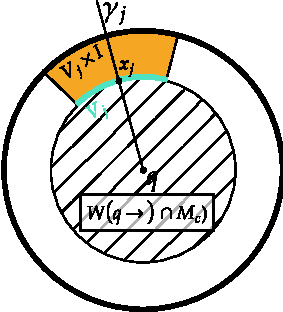
\includegraphics[width=3.8cm]{Text/Pictures/V_jTimesI}}% get height and width
		\hangafter \numexpr -\ht0/\baselineskip -1\relax% adds one blank lines at bottom
		\hangindent \dimexpr \wd0 + 1.2em\relax% adds 1em margin on right
		\vbox{\raisebox{-\height}[0pt][0pt]{\hspace{0.2em}\box0}}\vspace{-1.2ex}% overlap image
For this we make use of an collar neighbourhood of $W(q\to )\cap M_c$ defined as follows:	Again using the implicit funktion theorem and spherical coordinates (compare \color{red}referenz \color{black}) we have that the preimage of $W(q\to )\cap M_c$ under the embeddign $E^u_q: T^u_qM\to W(q\to)$ is (after rescaling the funktion) a Disk, So withour restrictions assume that $E^u_q(B_1(0))=W(q\to )\cap M_c$. Then $\mathfrak{C}\coloneq E^u_p(B_2(0))$ is a collar neighbourhood and $V_j\times I\hookrightarrow L_i\subseteq \mathfrak{C}$ embedds in the obvious way. This is done by mapping $V_j\times I$ fisrst into $B_2(0)$ via $(v,t)\mapsto (E^u_q)^{-1}v\cdot (1+t)$ and then applying $E^u_p$. 
	\end{minipage}
	
This mapping $E^u_q$ gives also rise to an oriented chart of $V_j$: For this we deform $B_2(0)$ to be a cylinder along $\gamma_j$ by changing the base such that $(E^u_q)^{-1}x_j$ is the first base vector whilst keeping the orientation ($\det$ of base change is one). Then just strech the disc:
 \begin{equation*}
 	(x_1,\dots x_{\lambda_{p}+1})\mapsto (\frac{x_1}{|x_1|},\dots x_{\lambda_{p}+1})\, .
 \end{equation*}. By transversality of $V_j$ and $\gamma_j$ we can assume that the orthogonal projection $\Pi_j$ along the first basis vector restricted to the preimage of $V_j$ is a homeomorphism. Now we get the chart as a composition:
 \begin{align*}
 	E^u_{q,j}\coloneq  \Pi_j\circ (E^u_{q})^{-1}: V_j \to \R^{\lambda_{p}} 
 \end{align*}
  Here is where the definition of the Morse boundary operator comes because now we have two different orientations in $V_j$. One induced from $T^u_pM$ (lets call the oriented basis $b^u_p$) and one induced from above. Hence in $Tx_j\gamma_j\oplus Tx_jV_j$ we have two different oriented basis induced from this chart and from the chart given by the tubular neighbourhood embedding of $W(\to p)\cap M^c$ restricted to the normal fiber above $x_j$.
  \begin{center}
% https://tikzcd.yichuanshen.de/#N4Igdg9gJgpgziAXAbVABwnAlgFyxMJZABgBpiBdUkANwEMAbAVxiRAB12AlAPWE4Z0AtgCModAPpoAviGml0mXPkIoAjOSq1GLNgBUeTKQFk5CkBmx4CRMmq31mrRCABqEgFZytMKAHN4IlAAMwAnCCEkDRAcCCQyEEERGAYABSVrVRAsMGxYEGpHXRcARwlgEUMpWXkQ8MjEACZqWKjCnWcQAClOESw-AB9ygFVygA9PaWk+AFo1WWoklPSrFTZQ-oALHDM6iKRmmLjEBKLOgAoAUSrgEo9pAEoCxLpktIy1lwYYYJ3pCmkQA
\begin{tikzcd}
	\R^{\lambda_p}                                                   & T^u_pM \arrow[l, "q_{b^u_p}" description] \\
	V_j \arrow[ru, "J\big|_{U_{x_j}}^{-1}"'] \arrow[u, "(E^u_{qj})"] &                                          
\end{tikzcd}
  \end{center}
  If we now swich to the Alexandrof kompakitifikations we have that this diagramm kommutes up to homotopy, if and only if the orientaions agree. \todo{hier beweis nachholen. Sollte eine einfache übuingsaufgabe sein mittels abbildungsgrad zwischen sphären ist homotopieinvariante}. Else we have a change of sign. Hence we have the diagramm that commutes up to sign: 
  
  \begin{center}	
 % https://tikzcd.yichuanshen.de/#N4Igdg9gJgpgziAXAbVABwnAlgFyxMJZABgBpiBdUkANwEMAbAVxiRAGUAdTmmGAAnYA9YNwZ0AtgCModAPpoAviEWl0mXPkIoAjOSq1GLNtwBmAJzoBjYAGE5O-gBUhTBQFlFozmjrm8jPz2ji5uaJ4qaiAY2HgERGQ6BvTMrIggZpY2wfwAanIAVl7cvv5YgTn5RSoGMFAA5vBEoBYQEkh6IDgQSGQg4lIwDAAKGnHaIOZY9QAWOCDUKcbp3FhQ-Ny8AgCOcsBSrgrKqi3mbUgATNTdHYtGaRmcaxucEGjMcPwAUtxS0wA+ewAqnsAB6FRSKEQAWh0ymoAyGo1iWjYU1m8xOIFa7UQVy6PUQfSWD1W602fH4AAoAKKHYDbIoASgW-TogxGY1R6QYMFMmIoiiAA
 \begin{tikzcd}
 	S\vee S^{\lambda_p}                                                                                               & \frac{C_1 T^u_pM}{\partial C_1 T^u_pM} \arrow[l, "\id \vee q_{b^u_p}"'] \\
 	\frac{C_1 V_j}{\partial C_1 V_j} \arrow[ru, "\id \oplus J\big|_{U_{x_j}}^{-1}"'] \arrow[u, "\id \vee (E^u_{qj})"] &                                                                        
 \end{tikzcd}
  \end{center}
  
Here the right path coincides with the path $f_2\circ f_1$. Now we introduce a left part that will later factor over the collaps that induces $\kappa_j$:
\begin{center}
	% https://tikzcd.yichuanshen.de/#N4Igdg9gJgpgziAXAbVABwnAlgFyxMJZARgBoAGAXVJADcBDAGwFcYkQBlAHS9phgAEHAHrAejegFsARlHoB9NAF8QS0uky58hFACYK1Ok1bseAMwBO9AMbAAwvOICAKsOaKAskrFc09C3hMAg5Oru5oXqrqIBjYeAREZMSGDCxsiCDmVrYhAgBq8gBW3jx+AVhBuQXFURpx2kTkBjSpJhkAcvIAjiEAFAAy3QCUqoYwUADm8ESglhCSSE0gOBBIZCAS0jCMAAqa8TogWGDYsCAtxumZXFhQAjx8gtJuirUgcwuI6ytI+kZpphudx4EDQLDgAgAUjxpFgJgAfeTAACqSIAHkUlCo1LMLPNFjQfog-q0rjxbvdePwBL0AKIvYBdYpDUQAWmIKhom22e3qCQyFjhAAscG8PgTlqtEABmC4AjJmeQAVnOG3oW12+waAuFopx7zxn1lkt+NC2YCgSFZ0qWpPY1ggjAkaAQXPVPK1-JAgomItGSiAA
	\begin{tikzcd}
		N_qC_1(L_q) \arrow[rd, "collaps"', bend right] & S\vee S^{\lambda_p} \arrow[r, "\id \vee b^u_p" description] \arrow[d, "\id \vee (E^u_{qj})^{-1}"'] \arrow[l, "f_5"'] & \frac{C_1 T^u_pM}{\partial C_1 T^u_pM} \arrow[ld, "\id \oplus J\big|_{U_{x_j}}"] \\
		& \frac{C_1 V_j}{\partial C_1 V_j}                                                                                     &                                                                                 
	\end{tikzcd}
\end{center}
We define $f_5$ as follows:
\begin{align*}
	f_5: S\vee S^{\lambda_p}= \frac{B_2(0)}{\partial B_2(0)} &\to N_qC_1(L_q)\\
	x&\mapsto \begin{cases}
		E^u_q(x)& \text{if } \norm{x}\leq 1\\
		(\lambda,x_j)& \text{if } x=(\lambda+1)\cdot x_j\text{, where }\lambda>0 \text{ and }x_j\in 	(E^u_q)^{-1}(V_j)\\
		p& \text{ else}.
	\end{cases}
\end{align*}
Now the left side commutes and also factos over the collaps that induces $\kappa_j$.\textit{ hence $\kappa_j$ is up to homotopie the plus or minus the identity which is determined by the sign of the Morse boundary operator at $\gamma_j$}. Now lets collect all:

The (trivialized) tubular neighbourhood embedding 
\begin{align*}
	J: W(p\to)\cap M^c\cong W(p\to)\cap M^c\times T^u_pM \to N_p
\end{align*}
together with collapsing $W(\to p)\cap M^c$ (which is realiced by the projection $\pi: W(p\to)\cap M^c\times T^u_pM\to T^u_pM$) and a koordinate map $q$ induced by a basis of $T^u_pM$ gives rise to a map:
\begin{align*}
	T\coloneq q_{b^u_p}\circ \pi\circ J^{-1}: N_p\to \R^{\lambda_{p}}
\end{align*}
This gives rise to a well defined map 
\begin{equation*}
	\tilde{T}: \frac{N_p}{L_p}\to \overline{\R^{\lambda_{p}}}\cong S^{\lambda_p}; \tilde{T}(x)=\overline{T(x)}
\end{equation*}which again can be extended to a map which we will call $T$ by abuse of notation: 
\begin{align*}
T\coloneq \id\vee \tilde{T}: S_1\vee \left(L_q\cup N_p \middle/  L_p \cup \cl (L_q \setminus {N_p})\right) \to S^{\lambda_p+1}
\end{align*} 

 Hence, the Morse datum together with $T$ gives rise to a natural generaor of $K^{\lambda_p-1}\left[L_q\cup N_p ,  L_p \cup \cl (L_q \setminus {N_p})\right]$. Furthermore the map  $\left((c_j\circ \Lambda)^*\right)_j^{-1}\circ c_{\iota}^*\circ (\eta^*)^{-1}\circ \gamma^*\circ T$ commutes with the map $\id \vee b^u_p\circ (\id \oplus J\big|_{U_{x_j}})$. To see this notice how $\eta$ and $\gamma$ are just the identity. Furthermore $c_\iota$ is, and $\left((c_j\circ \Lambda)^*\right)_j^{-1}$ is induced by the inclusion of $C_1V_j\big/ \partial C_1V_j$ into the space $C_1L_q\big/ \cl\left(C_1(L_q)\setminus \bigcup\limits_{j=1}^lC_1V_j \right)$. Hence the composition reads
 \begin{align*}
\left((c_j\circ \Lambda)^*\right)_j^{-1}\circ c_{\iota}^*\circ (\eta^*)^{-1}\circ \gamma^*
=\left(\gamma \circ \eta^{-1}\circ c_{\iota}\circ i\right)^*\\
=\left[x\mapsto \begin{cases}
	p & \text{ if }x\in N_q\cup N_p\cup C_1\left(L_q\cup \cl\left(L_q\setminus \bigcup\limits_{j=1}^lV_j\right) \right)\\
	x & \text{ else .}
\end{cases}\right]^*
 \end{align*}  Now the collapsing reqirement is much easyer in reality, is $x$ comes from $C_1V_j$ because: 
 \begin{align*}
 	C_1V_j \bigcup N_q\cup N_p\cup C_1\left(L_q\cup \cl\left(L_q\setminus \bigcup\limits_{j=1}^lV_j\right) \right)= \partial C_1V_j 
 \end{align*} With this in mind, the whole composition equals:
 \begin{align*}
 	q_{b^u_p}\circ \pi \circ J^{-1}\circ \gamma \circ \eta^{-1}\circ c_{\iota}\circ i=(\id \vee q_{b^u_p})\circ (\id \oplus J^{-1}) \, .
 \end{align*}
 Hence this composition equals $(id\vee J\big|_{U_{x_j}}\circ B_{b^u_p})^{-1}$. Now lets stich everything together and let $p$ be a generator of $K^{\lambda_p-1}\left[L_q\cup N_p ,  L_p \cup \cl (L_q \setminus {N_p})\right]$ induced by $T$ and the orientation of $T^u_pM$. (This means that $p=T^*(\beta)$, where $\beta$ is the Bott generator of $K^{\lambda_p-1}[S^{\lambda_p-1}]$). Then:
\begin{align*}
	\delta_{triple}(p)
	&=(m^*)^{-1}\circ \underbrace{c^*\circ i_{\delta}^*\circ i_{\eta}^*}_{=\sum\limits_{j=1}^l\kappa _j\circ \pi_j}\circ c_{\iota}^*\circ (i_{\eta}^{-1})^*\circ \gamma^*(p)\\
	&=(m^*)^{-1} \circ \sum_{j=1}^{l}\left(\kappa_j\circ \pi_j\circ c_{\iota}^*\circ (i_{\eta}^{-1})^*\circ \gamma^*\right)(T^*(\beta))\\
	&=(m^*)^{-1} \circ \sum_{j=1}^{l}\left(\kappa_j\circ (\underbrace{q_{b^u_p}\circ \pi\circ J^{-1}\circ \gamma \circ i_{\eta}^{-1}\circ c_{\iota}\circ i_j}_{=(\id \vee q_{b^u_p})\circ (\id \oplus J^{-1})})^*(\beta)\right)\\
	&=(m^*)^{-1} \circ \sum_{j=1}^{l}\left(\kappa_j((\pm)_{\gamma_j}(\id\vee E^u_{qj})^*(\beta)) \right)
\end{align*}
 Now we give its image a canonical generator induced by a basis of $T^u_qM$. For this we need a map $S^{\lambda_p+1}\to N_q\big/ L_q$ that commutes with $(m^*)^{-1} \circ f_5$. Once we have this we are finally done!!!
 	This however can be done easily. For this we make use of the unstable manifold theorem and rescale the immersion such that $W(q\to )\cap M_c$ is the image of the Ball $B_0(1)$. Furthermore,  $N_q\slash L_q\simeq W(q\to )\cap M_c$ since it is a tubular neighbourhood. Hence we get a map 
 	\begin{align*}
 		(E^u_q):  S^{\lambda_p+1}\to N_q\slash L_q
 	\end{align*} Now $(E^u_q)\simeq (m\circ f_5)\simeq \id$ since  $(E^u_q)^{-1}\circ (m\circ f_5)\simeq \id$. The latter is clear due to the first being just a streching $B_0(1)\to B_0(2)$ and then collaps of the outer ring. This composition however obvieously is homotopic to the identity. 
 	Hence $(E^u_q)^*\circ (m^*)^{-1}=f_5^*$ .
 	
 	Now we apply $(E^u_q)^*$ to the calculation above to figure out the map:
 	
 	\begin{align*}
 	(E^u_q)^*\circ 	\delta_{triple}(p)
 	&= (E^u_q)^*\circ (m^*)^{-1} \circ \sum_{j=1}^{l}\left(collaps^* \circ (\pm)_{\gamma_j} (\id\vee E^u_{qj})^*(\beta) \right)\\
 	&= \sum_{j=1}^l (\pm)_{\gamma_j} f_5^* collaps^* \circ (\id\vee E^u_{qj})^*(\beta)\\
 	&=\sum_{j=1}^l (\pm)_{\gamma_j} \beta=n(p,q)\beta
 		 	\end{align*}
Or said differently by defining $q$ to be the generator of $N_q\big/L_q$ given by the orientation of $T^u_qM$ as $q=((E^u_q)^{-1})^*(\beta)$ then:
\begin{equation*}
	\delta_{triple}(p)=n(p,q)q\,.
\end{equation*} 	
 \todo{Uns interresiert wie viele q da rauskommen. Also eher eine Koordinatenmap nach dem tripple operator. Wenn ich die einfüre,dann könnte es passen? }
 
 
% https://tikzcd.yichuanshen.de/#N4Igdg9gJgpgziAXAbVABwnAlgFyxMJZABgBoAmAXVJADcBDAGwFcYkQBpAPTQAIAdHIP79GMAGY5kvGcKFD+4gE70AxsF4BhAPoBGABQAZbQEcAlAF8B8ubw0jVjWTfnWRYyfrcvvOg8fMROBgcAFssMGY4AX4AIywAc1VmNHcscJw4bWAAKwBeXQsuJz8ANW0c5zlBN34lRIALHDMqnytqusacShALUnRMXHxCFF0KajomVnZuVNEJKTKKmPiEgHoYtHolPCYtPV5ynJF6hKaevoHsPAIiMl0JhhY2RE4edwXkADlTBxTeH5zZJ8PxGX78YEA7RoMwnLoXfogDDXYZEcikB40J7TV6zD6SZB+AAqXGY0IAsitEhsRFsdlg9n5eCSyWhKXCzt1eojkUNbigyMRHlMXm85h4pD8TFT1mDAp1OQirnyRsgxkKsSKZjxkAARUnZEQwNDYRgECwiVZrWnbXZOfVk4BGk1YM1gKxKpGDG6q9EaybPbVoZAAZS4TtE9FCsSg9GhAGpCp7eT6iGNMQGcWLkCJlGpgAAhbTkfTESwRul23hFktliwXCYwKAJeBEUDKCChJBkEA4CBIciXEAdruIMa9-uIdGZ0UiADW9DQWxANEY9FiMEYAAVvajXqcmtz20pO0hx33u0OR0gAMw0C9jzWB17iYtH4cn0fTh8AFivn6QH970nABWf9T0QEDgKQAA2J8s1fH932vKdoMg+DRVfG9kIAxA4InW8MPYV9dBwiCAHY0LvGd2FiPQyNHSiCPQmjXjo8gVxAOAGiwSRL0RFCmIfcdsVneZPH0ABRA1zHDABaQoHCwJRVF4LAOSaMwuAAKk4tcN23Xd+RACJsFgXpKAsIA
\begin{tikzcd}
	{K^p\left[N_q \big/(L_q)\right]} \arrow[r]                                                                                                                      & {K^p[D^u_{\epsilon}\big/\partial D^u_{\epsilon} ]} \arrow[r, "f_4"]                                                                 & {K^p[S^{\lambda_p+1}]} \arrow[d, "f_1"]                                  \\
	{K^p\left[N_q\cup N_p\cup C_1(L_q\cup N_p)\right]} \arrow[u] \arrow[ru, "f_3"]                                                                                  & {K^p[\frac{B_2(0)}{\partial B_2(0)}]} \arrow[r, "b_1"] \arrow[u, "b_2"] \arrow[d, "\left((E^u_q)^{-1}\circ i\right)^*" description] & {K^p\left[C_1T^u_pM \big/ \partial C_1 T^u_pM \right]} \arrow[ld, "f_2"] \\
	{K^p 		\left[   			\frac{ C_1(L_q)} 				 { \cl  				 	\left( 				 		C_1(L_q)\setminus \bigcup\limits_{j=1}^l C_1V_j  				 	\right)  				 } 		\right]} \arrow[u] & {K^p\left[C_1V_j \big/ \partial C_1 V_j\right]} \arrow[lu, "\kappa_j"'] \arrow[l]                                                     &                                                                         
\end{tikzcd}
Now we start going arround that diagramm wich is commutative up to hopotopie and start at the bottom. $b_1$ is the same map as $f_1$ and hence makes use of the orientation of $T^u_pM$. $f_2\circ b_1$ is homotopic to the inculsion induced mapping $\left((E^u_q)^{-1}\circ i\right)^*$. This can be seen as follows: First notice how $f_2\circ b_1$ is homotopic to map induced from $(\id\oplus E^u_{q,j})^{-1})$
\begin{equation*}
	(x_1,\dots x_{\lambda_{p}+1})\mapsto (\frac{x_1}{|x_1|},\dots x_{\lambda_{p}+1})\, .
\end{equation*}
now the half cylinder ($x_1\geq 0$) is again homotopic to the whole with the inclusion and collapsing being the homotopic invers maps. Those considerations also work modulo the boundary. Now $f_2\circ b_1$ is homotopic to $\left((E^u_q)^{-1}\circ i\right)^*$ if and only if the chart $(E^u_q)^{-1}$  by applying the streching map $s:\frac{B_2(0)}{\partial B_2(0)}\to \frac{B_2(0)}{\partial B_2(0)}$: (which is homotopic to the identity.)
\begin{center}
	
	
	\tikzset{every picture/.style={line width=0.75pt}} %set default line width to 0.75pt        
	
	\begin{tikzpicture}[x=0.75pt,y=0.75pt,yscale=-1,xscale=1]
		%uncomment if require: \path (0,300); %set diagram left start at 0, and has height of 300
		
		%Shape: Block Arc [id:dp2516942430671658] 
		\draw  [fill={rgb, 255:red, 245; green, 166; blue, 35 }  ,fill opacity=1 ] (284,83.96) .. controls (298.88,68.69) and (319.24,58.69) .. (342.17,57.27) .. controls (351.83,56.67) and (361.22,57.63) .. (370.11,59.95) -- (362.53,89.26) .. controls (356.65,87.73) and (350.44,87.08) .. (344.05,87.48) .. controls (328.89,88.42) and (315.43,95.05) .. (305.6,105.17) -- cycle ;
		%Shape: Ellipse [id:dp31830895843634066] 
		\draw  [line width=2.25]  (258.59,146.8) .. controls (258.59,97.56) and (298.5,57.65) .. (347.74,57.65) .. controls (396.97,57.65) and (436.89,97.56) .. (436.89,146.8) .. controls (436.89,196.04) and (396.97,235.95) .. (347.74,235.95) .. controls (298.5,235.95) and (258.59,196.04) .. (258.59,146.8) -- cycle ;
		%Shape: Ellipse [id:dp9709870130157104] 
		\draw   (288.6,146.8) .. controls (288.6,114.14) and (315.08,87.66) .. (347.74,87.66) .. controls (380.4,87.66) and (406.87,114.14) .. (406.87,146.8) .. controls (406.87,179.46) and (380.4,205.93) .. (347.74,205.93) .. controls (315.08,205.93) and (288.6,179.46) .. (288.6,146.8) -- cycle ;
		%Shape: Circle [id:dp482439832706389] 
		\draw  [draw opacity=0][fill={rgb, 255:red, 0; green, 0; blue, 0 }  ,fill opacity=1 ] (348.7,143.89) .. controls (349.7,143.43) and (350.88,143.87) .. (351.33,144.87) .. controls (351.79,145.87) and (351.35,147.04) .. (350.35,147.5) .. controls (349.35,147.95) and (348.17,147.51) .. (347.72,146.51) .. controls (347.27,145.52) and (347.71,144.34) .. (348.7,143.89) -- cycle ;
		%Shape: Arc [id:dp1835190035098445] 
		\draw  [draw opacity=0][line width=2.25]  (305.17,104.91) .. controls (315.42,94.49) and (329.49,87.79) .. (345.25,87.13) .. controls (351.39,86.87) and (357.36,87.55) .. (363.01,89.04) -- (347.74,146.8) -- cycle ; \draw  [color={rgb, 255:red, 80) -- (423.42,97.86) ;
			%Straight Lines [id:da15646287377542745] 
			\draw    (320.32,61.14) -- (397.42,70.86) ;
			
			%Straight Lines [id:da5095357448746147] 
			\draw    (323.57,61.6) -- (351.75,235.79) ;
			%Straight Lines [id:da6233786094876668] 
			\draw    (323.57,61.6) -- (321.84,230.24) ;
			%Straight Lines [id:da23916661666457828] 
			\draw    (322.57,62.6) -- (289.95,214.07) ;
			%Straight Lines [id:da33960840190709396] 
			\draw    (322.57,62.6) -- (270.05,186.5) ;
			%Straight Lines [id:da11039605607469682] 
			\draw    (322.57,62.6) -- (260.47,152.72) ;
			%Straight Lines [id:da5150377253833407] 
			\draw    (322.57,62.6) -- (265.75,115.61) ;
			
			% Text Node
			\draw (311.67,43.4) node [anchor=north west][inner sep=0.75pt]  [font=\scriptsize]  {$y_{j}$};
			
			
		\end{tikzpicture}
		
		\end{center}
		Using this streching we have that 
		\begin{minipage}{\dimexpr \textwidth-2\fboxsep-2\fboxrule}
		\abovecaptionskip=0pt
		\sbox0{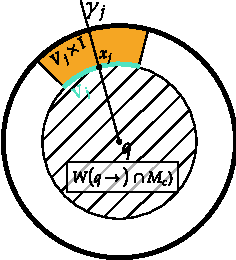
\includegraphics[width=3.8cm]{Text/Pictures/the rescaling with rays}}% get height and width
		\hangafter \numexpr -\ht0/\baselineskip -1\relax% adds one blank lines at bottom
		\hangindent \dimexpr \wd0 + 1.2em\relax% adds 1em margin on right
		\vbox{\raisebox{-\height}[0pt][0pt]{\hspace{0.2em}\box0}}\vspace{-1ex}% overlap image
		Furthermore, $V_j\times I$ is homeomorphic to $\mathfrak{C}$ by streching it. The streching can be done along rays starting in $y_j=(x_j,1)$. This is homotopic to the identity, if viewed as a endomorphism in $W(q\to)\cap M_c$. We can now define the collapsing map $W(q\to)\cap M_c$ in a continouos way by defining it to be the identity inside of $L_j$ and outside we map each point to the intersection of the ray containing said point with the bundary of $L_p$.
		Das solworklte die letzte Lücke sein!
		\end{minipage}
	\end{proof}; green, 227; blue, 194 }  ,draw opacity=1 ][line width=2.25]  (305.17,104.91) .. controls (315.42,94.49) and (329.49,87.79) .. (345.25,87.13) .. controls (351.39,86.87) and (357.36,87.55) .. (363.01,89.04) ;  
		%Shape: Ellipse [id:dp3336819844491399] 
		\draw  [draw opacity=0][fill={rgb, 255:red, 0; green, 0; blue, 0 }  ,fill opacity=1 ] (331.4,87.95) .. controls (332.4,87.49) and (333.57,87.93) .. (334.03,88.93) .. controls (334.48,89.93) and (334.04,91.11) .. (333.04,91.56) .. controls (332.05,92.02) and (330.87,91.58) .. (330.41,90.58) .. controls (329.96,89.58) and (330.4,88.4) .. (331.4,87.95) -- cycle ;
		%Straight Lines [id:da2883617960271355] 
		\draw    (320.32,61.14) -- (375.42,231.86) ;
		%Straight Lines [id:da6580977928561076] 
		\draw    (320.32,61.14) -- (399.42,218.86) ;
		%Straight Lines [id:da549347805026984] 
		\draw    (320.32,61.14) -- (420.42,196.86) ;
		%Straight Lines [id:da3542746287685834] 
		\draw    (320.32,61.14) -- (435.42,164.86) ;
		%Straight Lines [id:da38915223346361993] 
		\draw    (320.32,61.14) -- (435.42,130.86) ;
		%Straight Lines [id:da011207389658813405] 
		\draw    (320.32,61.14
\end{comment}
\begin{proof}[Commuting triple connecting homomophisms]
	We first notice, that we have the map of triples given by the inclusion:
	\begin{align*}
		\left( ~W(q\to)\cap N_q ~,~S(q\to)~,~S(q\to ) \setminus \bigcup\limits_jV_j ~\right) \to (C,B,A)
	\end{align*} and hence by naturalitiy we have the diagram, where the top square commutes:
	\begin{fdiagram}
% https://tikzcd.yichuanshen.de/#N4Igdg9gJgpgziAXAbVABwnAlgFyxMJZABgBpiBdUkANwEMAbAVxiRAGkA9YAWgB0+DOgFsARlDoB9NAF8BDGADMcyAAQAhUgEFVAgE5YA5gAscFEDNLpMufIRQBGclVqMWbLr3kjxUgI5ygkoqAMKkGrp8BiZmFlYgGNh4BERkDi70zKyIHNz8gj4S0oEKymoAygAUfgI4EACUpFU1fHX1AnAwOMJYYExwkaJGAMZMaPJYPThwkgBWkb14lQBqc-WR0abmltZJdkRO6dSZ7jme+UJiRQHywcgA6tW1DQLDdGiqAHLSTU+tDRsjFs4rtbCkUGQAEwZNzZXJeApXKSyW5lVSrWakARoOh6PCMdFzQExbYuGBQQzwIigRR6CDCJBkEB1JBOEBCUQwBgABRsyXs7OCIGOsLYAlgDBwUmAOAMaAUMk4DhBIFp9MZ1BZiEhIqybCwkmAmi0ioAVCq1QzEGytQBmXWnEAG4BhdRmi10q065kQJD21x6nLirlSw2yrDymCKyEe9XazW+xAAFgdcINs045uoHK5vL24JAmxwwpAcGMWGUSEhO1VnqQKZ9ftTYr4EqlnFmYblCpLOZ5fP2OSLsatDa13pOcOGc0zvbonP7+YFw5kFBkQA
\begin{tikzcd}
	{K^{-\lambda_p}\left[ B,A \right]} \arrow[r, "\delta_{triple}^1"] \arrow[d, "{i_{B,A}^*}"]                                                            & {K^{-\lambda_q}\left[C, B \right]} \arrow[d, "{i_{C,B}^*}"] \\
	{K^{-\lambda_p}\left[ S(q\to),S(q\to)\setminus \bigcup\limits_j \inti(V_j) \right]} \arrow[r, "\delta_{triple}^2"] \arrow[d, "i_j^*"', shift right=2] & {K^{-\lambda_q}\left[W(q\to)\cap N_p,S(q\to) \right]}       \\
	{K^{-\lambda_p}\left[ V_j,\partial V_j \right]} \arrow[ru, "\delta^j_{triple}"'] \arrow[u, "c_j^*"']                                                  &                                                            
\end{tikzcd} 
	\end{fdiagram}
\noindent	Furthermore, in this diagram the tuple $\left(K^{-\lambda_p}\left[ S(q\to),S(q\to)\setminus \bigcup\limits_j \inti(V_j) \right],\left(c_j^*\right)_j\right)$ is a coproduct, and we define  $\delta^j_{triple}\coloneq \delta^2_{triple}\circ c_j^*$. Then we have that 
\begin{equation*}
	\delta^2_ {triple}=\sum_j\delta^j_{triple}\circ i_j^*
\end{equation*}
	
	The map $\delta^2_{triple}$ is defined as the composition:
	\begin{fdiagram} \label{diag: Definitino of delta j}
			\begin{adjustbox}{max width=\textwidth}
	% https://tikzcd.yichuanshen.de/#N4Igdg9gJgpgziAXAbVABwnAlgFyxMJZABgBoBGAXVJADcBDAGwFcYkQBpAPWAFoAdfo3oBbAEZR6AfTQBfQYxgAzHMgAEAZQAUAR0E4IASlLa9-A4cFwYOEVjDM4awWKwBzAMbM0CrHZxwUgBWzvz2eFoAasGGoQBO7gAWOJQgsqTomLj4hChkAEzUdEys7Nx8CqIS0nIKyqqauvpG8UkpaRkgGNh4BETkpIU0DCxsiJw8AkJVkjIA1OTyQvXIGlLkgrQwMI1mFq1uyanpmT05RPmDRSOl4+VTwuKzaAtLiirIAOpN5kaCHvQ0GoAHIyf7eNQAYXWdRUWl2zUs-AShxwxm+ez+-ABQNBQMEKKOHVO2T6KAAzFdhiUxhMKtMnjVXrDVBjEf9ASCwdiIdCNss4QjfkjCWiCW1jp1uqTcshKVRqaMypNKoypDo3is2cKObiZCYfvtxajJSTerKyMRrjTlfTHtUZJqPmpokFSII0PQ4ngmC7ggcibIijAoG54ERQEo4hAREgyCADEgBsUleMsOsuAAqYkgKMxpM0ROIS4p24gRJZ9Y5vOx4uFiBISml2mJKT5LPV6O1ptFgAsirL6fb2ZOua7SH7CYbiAArAPaS4bPR-lg4h5QjgYAAPHDAHAJWiyKTAPmmRGyTv5xDxotz5vsQSwRg4ehcfLH-dYNCKC+jmtIAA2es43ndgPGCDsg1kIA
	\begin{tikzcd}
		{K^{-\lambda_p}\left[ V_j,\partial V_j \right]} \arrow[d, "c_j^*"]                                                                      &                                                                    &                                                                                                                 &                                                                                                                              \\
		{K^{-\lambda_p}\left[ S(q\to),S(q\to)\setminus \bigcup\limits_j \inti(V_j) \right]} \arrow[d, "i_1^*"] \arrow[rrr, "\delta^2_{triple}"] &                                                                    &                                                                                                                 & {K^{-\lambda_q}\left[W(q\to)\cap N_p,S(q\to) \right]}                                                                        \\
		{K^{-\lambda_p}\left[ S(q\to) \right]} \arrow[r, "h^*_1"]                                                                               & {K^{-\lambda_p+1}\left[S_1\vee S(q\to) \right]} \arrow[r, "h_2^*"] & {K^{-\lambda_p+1}\left[W(q\to)\cap N_p\cup C_1\left( S(q\to)\right),W(q\to)\cap N_p \right]} \arrow[r, "i_2^*"] & {K^{-\lambda_p+1}\left[W(q\to)\cap N_p\cup C_1\left( S(q\to)\right)\right]} \arrow[u, "\beta\circ \text{triv}_{C_1S(q\to)}"]
	\end{tikzcd}
			\end{adjustbox}
	\end{fdiagram}

The downwards maps in the Theorem are the induction of the canonical generators. This is done by the following assignement
	
	
	
	Now the composition \begin{equation*}
		h_1*i_1*\circ c_j*: K^{-\lambda_p}\left[ V_j,\partial V_j \right] \to K^{-\lambda_p+1}\left[S_1\vee S(q\to) \right]
	\end{equation*} can be simplified by the map
	\begin{equation*}
	l^*:	K^{-\lambda_p}\left[ V_j,\partial V_j \right]=K^{-\lambda_p+1}\left[S_1\vee\left( V_j,\partial V_j\right) \right] \to K^{-\lambda_p+1}\left[S_1\vee S(q\to) \right]
	\end{equation*} where l is the collapsing map.
	\begin{align*}
		l:S_1\vee S(q\to)  \to S_1\vee\left( V_j,\partial V_j\right)\\
		(t,x)\mapsto (t,\overline{x})
	\end{align*} So now we are in the following situation: 
	\begin{fdiagram}
		\begin{adjustbox}{max width=\textwidth}
% % https://tikzcd.yichuanshen.de/#N4Igdg9gJgpgziAXAbVABwnAlgFyxMJZABgBpiBdUkANwEMAbAVxiRAGkA9YAWgB0+DOgFsARlDoB9NAF8BDGADMcyAGqSAVqQFo6AJzyMABOo1GBerAHMAFjgogZpdJlz5CKAEzkqtRizYuXnkRcSkARzlBJRUAdQAKcPM+HAgjAEoBAGM6NCMAOWlSAGVEgVTMvktbe0dnEAxsPAIib09femZWRA5ufkFQiWkeAEYohWVkAWE6HBtRUWBimW4QsSG0AGox5Oq7BycXJvciMnbqToCeoP6hdak0UfGYqb4ZuYWlleA1sOltmS7az7OpHNwtFAjUgjDr+bq9YIDe7-MbyF5GYqSEYCGgwGAYsopCCVPa1GS+GBQKzwIigRR6CDCJAAZmoqSQZD8XTYimknAAVKCQPTGUhvCB2YgoVyrsLJOEBUKRUzEJzJdLLvCBLAGDg6JwNJJgDhLGgFDIlQyVayJRAxYdhVaWWy7YgACwXOFsOCKh3KpAe21iz3cnp6X31f2ql0BkOyhhYiN0p3umNSuPwhOeRwUGRAA
\begin{tikzcd}
	{K^{-\lambda_p}\left[V_j,\partial V_j \right]} \arrow[rr, "\delta^j_{triple}"] \arrow[rd, "l_1^*"]        &                                                                                     & {K^{-\lambda_q}\left[W(q \to )\cap N_p,S(q\to)\right]}                       \\
	& {K^{-\lambda_p+1}\left[ S_1\vee S(q\to)\right]} \arrow[rd, "r^*"] \arrow[ru, "l_2"] &                                                                              \\
	{K^{-\lambda_p-1}\left[\mathbb{S}^{\lambda_p+1} \right]} \arrow[uu, "f_p^*"] \arrow[rr] \arrow[ru, "s^*"] &                                                                                     & {K^{-\lambda_p-1}\left[\mathbb{S}^{\lambda_p+1} \right]} \arrow[uu, "f_q^*"]
\end{tikzcd}
		\end{adjustbox}
	\end{fdiagram}
		Now we have a list of the Functions from the diagramm above:\todo{Achtung hier stimmt was nicht... ich muss $f_p$ noch mit $\beta$ composen oder im diagramm etwas ändern.}
	\begin{itemize}
		\item The map $f_p$ induces $\alpha_p$. Remember, that $\alpha_p$ comes from the canonical generator $\alpha_p'$ of the index pair $[B,A]$ and $\alpha_p'$ is defined as
		\begin{align*}
			(\phi\circ{ \tilde{\psi}}^{-1})^*(\beta)~\text{where }& \phi \text{ is the homotopie equivalence of index pairs}\\
				& \tilde{\psi} \text{ is a Morse chart adapted to the basis of } T^u_pM,\\
				\text{and }& \beta \text{ is the bott generator of the sphere } [D^u_\epsilon\times D^s_\epsilon\Big/ \partial D^u_\epsilon\times D^s_\epsilon
\,				.
		\end{align*} Instead of using $\phi$ we can rescale $\tilde{\psi}$ to be a mapping to $[B,A]$ instead of first mapping to the prototype index pair $[D^u_\epsilon\times D^s_\epsilon,\partial D^u_\epsilon\times D^s_\epsilon]$. 
		We call this rescaled Morse chart $\psi$. 
		Then $\psi^{-1}(\beta)= (\phi\circ{ \tilde{\psi}}^{-1})^*(\beta)$ since the map $\tilde{\psi}\circ \phi^{-1}\circ \psi^{-1}$ has the local and hence global degree one. (this can be checkt by differentiataion at the origin). Hence $\alpha_p'=(\psi^{-1})^*(\beta)$. The inclusion 
		\begin{equation*}
			i_p: (V_j,\partial V_j)\to (B,A)
		\end{equation*} induces an isomorphism in the K-groups since $N_p$ is a tubular neighbourhood of the contractible $W(\to p)\cap M^c$ and the contraction to the fiber $V_j$ contracts $L_p$ to $\partial V_j$ (the contraction is well defined on the quotients, and for K-THeory, we only care for the qutoient spaces). Now $\alpha_p''=i_p^*(\alpha_p')$. Define the two funktions
		\begin{align*}
			J: \mathcal{N}^{W(q\to)} W(\to p)\cap M^c \to N_p \text{ the normal neighbourhood embedding,  }\\
			\nu: \mathcal{N}^{W(q\to)} W(\to p)\cap M^c \to  W(\to p)  \times T^u_pM \text{ The trivialization of the normal bundle.}  
		\end{align*}
		Define $\mathfrak{b}^p$ to be an ordered basis of $T^u_pM $ that is compatible to the orientation of said tanged space. Then assume that $J$ is defined, such that 
		\begin{align*}
			\left(B_{\mathfrak{b}^p}^{-1}\circ \nu_{x_j}\circ J^{-1}\right)^*(\beta)=\alpha_p'' \,.
		\end{align*} If this is not the case just compose $J$ with a basechage of degree one. Now $\alpha_p''$ generates $K^{-\lambda_p}(V_j,\partial V_j)$. The latter is isomoprhic to $K^{-\lambda_p+1}(I\times V_j,\partial(I\times  V_j))$ by definition. Now we denote the suspensision is the wedge produkt with a sphere. Hence for $K^{-\lambda_p+1}(I\times V_j,\partial(I\times  V_j))$ we can induce the generator by the function
		\begin{align*}
			f_p: I\times V_j \Big/ \partial(I\times V_j) &\to S \wedge S^{\lambda_p}\simeq  S^{\lambda_p+1}\\
			(t,x)&\mapsto \Omega\left(t,	\Gamma\circ \left(B_{\mathfrak{b}^p}^{-1}\circ \nu_{x_j}\circ J^{-1}\right)(x)\right) \, .
		\end{align*} \todo{specify the isomorphism !}
	$\Gamma$ maps the disk modulo its boundary to a sphere and $\Omega$ maps the suspension of the sphere to the sphere one dimension higher. We abuse the notation a bit and identify the map $\left(B_{\mathfrak{b}^p}^{-1}\circ \nu_{x_j}\circ J^{-1}\right)$ with the one defined by quotiening out the boundary. We will leave out the quotiening in the notatino from now on to make the prove easyer to read. The invested reader should check, if the quotiend maps are always well defined! Now finally we have a little definition issue: In the diagramm we have that 
		\begin{equation*}
			f_p^*: K^{\lambda_p-1}[\mathbb{S}^{\lambda_p+1}]\to K^{-\lambda_p}[V_j,\partial V_j]\, ,
		\end{equation*}whilst at the moment, $f_p$ maps to $K^{-\lambda_p+1}(I\times V_j,\partial(I\times  V_j))$. Hence we need to compose this $f_p^*$ with the isomorphism that comes from the suspension axiom: 
		\begin{equation*}
			K^{-\lambda_p}( X)\cong K^{-\lambda_p+1}(SX)\,.
		\end{equation*}By abuse of notation we dont write that idetification and rather think of the top left corner as $K^{-\lambda_p+1}(I\times V_j,\partial(I\times  V_j))$.
		\item Again, we want $f_q$ to be the map that induces the generator of $K^{-\lambda_q}[W(q\to)\cap N_q,S(q\to)]$ which comes from the canonical generator of $[C,B]$ together with the inclusion. Again instead of first introducing the generator on the prototype index pair, we can use ${E^u_q}^{-1}$ instead of the Morse chart. Again we can argue here, that the local degree of changing between the two is one, since ${E^u_q}^{-1}$ is a refined morse chart which can be choosen to be adapted to the ordered basis $\mathfrak{b}^q$ of $T^u_qM$.´ Hence we can define $f_q$ to be the quotient map:
		\begin{align*}
			W(q\to)\cap N_q\Big/ S(q\to)& \to S^{\lambda_p+1}\\
			x& \mapsto \Gamma\circ  B_{\mathfrak{b}^q}^{-1}\circ {E^u_q}^{-1}(x)\,.
		\end{align*} Here $\Gamma$ maps the disk modulo its boundary to the sphere. 
		Hence $f_q=\left(B_{\mathfrak{b}^q}^{-1} \circ {E^u_q}^{-1}\right)^*:K^{}$
		\item The map $l_1$ is the collapsing map 
		\begin{equation*}
			S_1\wedge S(q\to)\to S_1 \wedge (V_j\big/ \partial V_j)
		\end{equation*}
		\item The map $l_2$ is not topologically induced. 
		\item The map $s$ is given by $f_p\circ l_1$. Again we abuse the notation and leave out the suspension isomorphism when 
		\begin{equation*}
			s^*: K^{-\lambda_p+1}[S_1\wedge S(q\to)]\to K^{-\lambda_p-1}[\mathbb{S}^{\lambda_p+1}]\,.
		\end{equation*}
		\item To find the map $r$ that fits the diagram (to make it commute) is the next goal. First we need to dig into $l_2$: From diagram \ref{diag: Definitino of delta j} we know that $l_2=\Sigma \circ \text{triv}_{C_1S(q\to)}\circ i_2^*\circ h_2^*$, Where $\Sigma$ denotes the suspension isomorphism. Hence, if the function $r^*$ makes the diagram commutative we need to ensure, that $f_q^* \circ r^*=l_2$. If we define the function 
		\begin{align*}
			col: W(q\to) \cap N_p \cup C_1  S(q\to) \to S_1 \wedge S(q\to) \,
		\end{align*} 
		to be the collision, of $W(q\to) \cap N_p $ to a point, then
		$i_2^*h_2^*=col^*$. Now while the function  $\text{triv}_{C_1S(q\to)}$ is not topologically induced, its inverse is. Lets call the collaps of $C_1S(q\to)$ $c_1$. Then since $\Sigma$ is a natural transformation we have 
		\begin{equation*}
		 f_q^*\circ r^*=l_2\Leftrightarrow c_1^*\circ f_q^*\circ r^*=\Sigma \circ col^*
		\end{equation*}
		Now all maps are topologically induced except $\Sigma$ and the latter is just used to geht the index in the $K$ group right. Hence, if $r$ would be such that
		\begin{equation*}
			r\circ f_q\circ c_1=col\,, 
		\end{equation*}then the requirement on the induced maps would be satisfied. We first however need to formulate a little lemma:
		\begin{lemma}
			Let $S^k\coloneq \{x\in \R^{k+1}|\norm{x}=1\}$, $H_+\coloneq\{x\in S^k|x_0\geq 0\}$ denote the upper hemissphere, $H_-$ the lower hemissphere,  $\pi:S^k \to D^k$ with $\pi(x_0,\dots,x_{k})=(x_1,\dots x_k)$ be the projection and $\Lambda$ be the homeopmorphism from $D^k\big/\partial D^k \to S^k$. Let furthermore $c_{Eq}:S^k\to \overline{H_+}\vee \overline{H_-}$ be the collaps of the equator, where $\overline{H_+}$ denotes the upper hemisphere modulo the equator and $\overline{H_-}$ is defined analog. Let finally $c_2: \overline{H_+}\vee \overline{H_-} \to \overline{H_+}$ be the collaps of the second summand and analogusly $c_1:  \overline{H_+}\vee \overline{H_-} \to \overline{H_-}$. Then we have that $\Lambda\circ \pi\circ c_2\circ c_{Eq}\simeq -\Lambda\circ \pi\circ c_1\circ c_{Eq}$, where de minus denotes any map homeomorphism of negative degree. 
		\end{lemma}
		\begin{proof}
			This lemma is the concrete version of a standart lemma that is often formulated along the lines: Let $q:S^k\to S^k\vee S^k$ be the collaps of the equator and $p_i$ be the projection to the $i$-th summand, then $p_1\circ q=-p_2\circ q$.  
		\end{proof}
		Now we need to transport our situation to fit the lemma. For this we will use the maps defined in the lemma above, and need a bunch of maps again: 
		\begin{itemize}
			\item Firts, the map $\rho$ is given by 
			\begin{align*}
				\rho: W(q\to)\setminus \{q\}&\to W(q\to)\cap f^{-1}(c)\setminus W(q\to)\setminus \{q\}\\
				x\mapsto \phi_{\tau(x)}(x)\,,
			\end{align*} and 
			\begin{align*}
				 \tau: W(q\to)\setminus \{q\} &\to \R\\
				x                  &\mapsto \tau(x) \text{ such that }f\circ \phi_{\tau(x)}(x) =c \, .
			\end{align*}
			\item $\Phi:S^{\lambda_q}\to W(q\to) \cap N_p\cup C_1S(q\to)$ is defined with a case distingtion. We define 
			\begin{align*}
				\restr{\Phi}{{H}_+}(x)&=E^u_q\circ B_{\mathfrak{b}^q}^{-1}\circ \pi(x)\\
				\restr{\Phi}{{H}_-}(x)&=(\euler^{\tau(y)},\rho (y))\text{ where }y=E^u_q\circ B_{\mathfrak{b}^q}(\pi_-(x)) \,.
			\end{align*}Notice, how this function is continuous and does not depend on the choice taken in the definition of $\rho'$. 
			\item $\Psi: S^{\lambda_q}\vee S^{\lambda_q}\to \left(W(q\to)\cap N_p \middle/ S(q\to)\right)\vee \mathbb{S}\wedge S(q\to)$ is given by mapping $x\mapsto \overline{\Phi(x)}$. The well definition is easy to see. 
			\item $p_i$ for $i=1,2$ denotes the projection onto the first or second summand in a pointed sum. 
			\item $C_{S(q\to)}:W(q\to)\cap N_q\cup C_1S(q\to) \to \left(W(q\to)\cap N_p \middle/ S(q\to)\right)\vee \mathbb{S}\wedge S(q\to)$ is the collaps of $S(q\to)$. 
			\item $R:\mathbb{S}^{\lambda_q}\to \mathbb{S} \wedge S(q\to)$ is defined to be $col\circ \Phi$ 
		\end{itemize}
		This gives the commutative diagram,
		\begin{fdiagram}
		\begin{adjustbox}{max width=\textwidth}
	% https://tikzcd.yichuanshen.de/#N4Igdg9gJgpgziAXAbVABwnAlgFyxMJZAJgBpiBdUkANwEMAbAVxiRAB12IaYAnBrGBjAAEgH0A1AF9OPGAAJO3PgKGixAWikgppdJlz5CKMgEYqtRizacAtnRwALAEbPgAZSkA9YJwZ1bZyg6MQBHbV19bDwCIjIAZgt6ZlZEDnZ7J1cPb192f0DgsIi9EAxooyIABnIkq1T0zJc3Tx8-AKCQ8J1S8sNYlFNSc2pk6zT5AHUAClDOHAgASkV2AGM6NHkAOTE0TlWmTYBhMVN3Wfmlnqj+42R40iq6lJt8mAAzHGmZufYFxf2G22uxWtiwUCgDBgAHp5Odfv9OLwsABzRw4RbXMoGGJ3B6UUb1NighzNHKcADuMCgKIU8MumMi2IqA3uw2e43SUM+3wufyWgM2O02dnBkJhcL5iPYyLRGNkMAUdlJ2U8lOptMlCKuUgsGvgRFA714EFsSBqIAWSCGlheaU4ABkOsF9lheKsVmgsCtVm6PasxMQQNR-M4YAwAAo4yppQTYWBY42m83UK2IMi2zmO510V3uz3evP+07BkCh8NRlnGEBx8GsJlJs2IB6WiApzMNAPAACi3RDdDDkejAxrYHj9dKjaQLbTABZCXb0hHHFhEyamza0wBWBvrpAZtMANl3ycQ89bSAA7AvOScPFKliUjXvENeL4gtzeGpwvSX+4PK1uNhawTE8mzfI8v1eX8g3-Cth2rECJ2fU8LTTN8xm-dgI2wUtyyHKtgLHOsdAoKQgA
	\begin{tikzcd}
		&                                                            &                                                                                                                                                                          & \left(W(q\to)\cap N_p \middle/ S(q\to)\right)                                                                                            \\
		&  W(q\to) \cap N_p\cup C_1S(q\to) \arrow[rr, "C_{S(q\to)}"] & \mathbb{S}^{\lambda_q} \arrow[ru]                                                                                                                                        & \left(W(q\to)\cap N_p \middle/ S(q\to)\right)\vee \mathbb{S}\wedge S(q\to) \arrow[u, "\pi_1" description] \arrow[d, "\pi_2" description] \\
		\mathbb{S}^{\lambda_q} \arrow[rr, "c_{Eq}" description] \arrow[ru, "\Phi"] &                                                            & \overline{H_+}\vee \overline{H_-} \arrow[u, "\Lambda\circ \pi \circ c_2" description] \arrow[d, "\Lambda\circ \pi \circ c_1" description] \arrow[ru, "\Psi" description] &  \mathbb{S}\wedge S(q\to)                                                                                                                \\
		&                                                            & \mathbb{S}^{\lambda_q} \arrow[ru]                                                                                                                                        &                                                                                                                                         
	\end{tikzcd}
		\end{adjustbox}
		\end{fdiagram}
		 Now define $r\coloneq -R$. For example apply $R$ after the reflection $(x_0,\dots x_{\lambda_q})\mapsto (-x_0,\dots,x_{\lambda_q})$. Then by the lemma above and commutativity we have up to homotopy:
		  \begin{align*}
		  	r\circ f_q\circ c_1 
		  	&=  	-R\circ f_q\circ c_1 \circ \Phi \circ \phi{-1}\\
		  	&=  	-R\circ \Lambda \circ c_2\circ C_{Eq} \circ \phi{-1}\\
		  	&=  	R\circ \Lambda \circ c_1\circ C_{Eq} \circ \phi{-1}\\
		  	&=		col\, .
		  \end{align*}
		  With $r$ we finally have all the maps. Now we want to find out what degree the composition
		  $s\circ r$ has. For this we calculate the local degree in some point by checking the sign of the determinant of the Jacobean.
	\end{itemize} 
	Bevor we start differentiating, we expand the map arround $x\in \R^{\lambda_q}$, such that $x'\coloneq E^u_q\circ B_{\mathfrak{b}^q}(x)\in \rho{-1}(x_j)$, meaning that $x'$ is on the flow line towards $x_j$ and assume that $\tau(x_j)=1$.
	\begin{align*}
		&   \phantom{=}	\pi_+\circ s\circ r\circ \pi_+^{-1}(x_1,\dots .,x_{\lambda_q})\\
		&=	\pi_+\circ s\circ R (- x_0,x_1,\dots .,x_{\lambda_q}) \quad x_0>0\\
		&=	\pi_+\circ s\circ col \circ \restr{\Phi}{H_-} (-x_0,x_1,\dots .,x_{\lambda_q}) \\
		&=	\pi_+\circ f_p\circ l_1 \circ col \left(e^{\tau(x')},\rho(x')\right) \quad \text{ $col$ and $l_q$ are the identity arround $\left(e^{\tau(x')},\rho(x')\right)$ } \\
		&=\pi_+\circ \Omega  \Big(e^{\tau(E^u_q\circ B_{\mathfrak{b}^q}(x))},\Gamma \circ \underbrace{B_{\mathfrak{b}^p}^{-1} \circ \nu_{x_j}\circ J^{-1}\circ \rho \circ E^u_q\circ B_{\mathfrak{b}^q}(x)}_{\coloneq Z(x)}\Big)\\
		&=\sin(\pi e^{\tau(E^u_q\circ B_{\mathfrak{b}^q}(x))}) \cdot
		\begin{pmatrix}
			-\cos\left(\pi \cdot \norm{Z(x)}\right)\\
			 \sin\left(\pi \cdot \norm{Z(x)}\right) \cdot \frac{Z(x)}{\norm{Z(x)}})
		\end{pmatrix}
	\end{align*}
	Here $Z$ is a funktion $Z: \inti(I\times D^{\lambda_q})\to \R^{\lambda_q-1}$ and we can calculate its jacobean Notice how $Z(y)=0$ where $y$ is the same as above. We only care for the sign of its jacobean, so we will manipulate the funktion in a way that might change the function, but not the sign of ots Jacobean determinant. 
	Let $Q_y: V\to T_yV$ be the canonical map, that identifies a linear space with the tangendspace of a point from inside said space. Now we calculate:
	
	
	\begin{align*}
		&\phantom{=}Q_0^{-1}\circ \restr{\diff \left(B_{\mathfrak{b}^p}^{-1} \circ \nu_{x_j}\circ J^{-1}\circ \rho \circ E^u_q\circ B_{\mathfrak{b}^q}\right)}{y}\circ Q_y (e_i)\\
		&=Q_0^{-1}\circ  \restr{\diff \left(B_{\mathfrak{b}^p}^{-1} \circ \nu_{x_j}\circ J^{-1}\circ \rho \circ E^u_q\right)}{B_{\mathfrak{b}^q}(y)}\circ Q_{B_{\mathfrak{b}^q}(y)}\circ B_{\mathfrak{b}^q}(e_i) \quad \text{ in general $Q$ and $\diff L$ has a commutative property}\\
		&= Q_0^{-1}\circ \restr{\diff \left(B_{\mathfrak{b}^p}^{-1} \circ \nu_{x_j}\circ J^{-1}\right)}{x_j}\circ \restr{\diff \left( \rho \circ E^u_q\right)}{B_{\mathfrak{b}^q}(y)}\circ Q_{B_{\mathfrak{b}^q}(y)}\circ B_{\mathfrak{b}^q}(e_i)		
	\end{align*}
	Now the term $\restr{\diff \left( \rho \circ E^u_q\right)}{B_{\mathfrak{b}^q}(y)}\circ Q_{B_{\mathfrak{b}^q}(y)}\circ B_{\mathfrak{b}^q}$ induces a basis in $T_{x_j}W(q\to)$ that is compatible with the basis induced from
	\begin{equation*}
 \underbrace{\pi_{-\grad_{x_j}(f)^\top}}_{\text{projects onto the orthogonal complement of }-\grad_{x_j}(f)}\circ \restr{\diff  E^u_q}{B_{\mathfrak{b}^q}(y)}\circ Q_{{E^u_q}^{-1}(x_j)}\circ B_{\mathfrak{b}^q}
	\end{equation*} To see this notice how $\rho\circ E^u_q(x)=E^u_q\circ A_{\tau\circ E^u_q(x)}(x)$. In the basis $\mathfrak{b}^q$ and with $y'\coloneq E^u_q\circ B_{\mathfrak{b}^q}(y)$, and $M\coloneq \diag(\mu_1,\dots,\mu_{\lambda_q})$ we can calculate:
	\begin{align*}
	&\phantom{=}\restr{\diff \left(B_{\mathfrak{b}^q}^{-1}\circ A_{\tau \circ E^u_q\circ B_{\mathfrak{b}^q}}\circ B_{\mathfrak{b}^q}\right)}{y}\\
		&=\underbrace{\restr{\diff_t \left( B_{\mathfrak{b}^q}^{-1}\circ A_{t}\circ B_{\mathfrak{b}^q}\right)}{t=\tau (y')}}_{=M\cdot B_{\mathfrak{b}^q}^{-1}\circ A_{\tau(y')}\circ B_{\mathfrak{b}^q}(y)}
		\cdot \underbrace{\restr{\diff_x \left(\tau \circ E^u_q \circ B_{\mathfrak{b}^q}\right)}{y}}_{=(-1,0,\dots,0)}
		+\underbrace{\restr{\diff_x B_{\mathfrak{b}^q}^{-1}\circ A_{\tau(y')}\circ B_{\mathfrak{b}^q}}{y}}_{=B_{\mathfrak{b}^q}^{-1}\circ A_{\tau(y')}\circ B_{\mathfrak{b}^q}}\\
\end{align*}	
This has the jacobean 
\begin{equation*}
		\begin{pmatrix}
			* &0\\
			*&Z
		\end{pmatrix}, 
\end{equation*} where $Z$ has a positive determinant. Hence, 
\begin{align*}
&\pi_{-\grad_{x_j}(f)^\top} \circ \restr{\diff  E^u_q}{B_{\mathfrak{b}^q}(y)}\circ Q_{{E^u_q}^{-1}(x_j)}\circ B_{\mathfrak{b}^q}\circ 		\begin{pmatrix}
	* &0\\
	*&Z
\end{pmatrix}\\
&= \pi_{-\grad_{x_j}(f)^\top} \circ \restr{\diff \left( \rho \circ E^u_q\right)}{B_{\mathfrak{b}^q}(y)}\circ Q_{B_{\mathfrak{b}^q}(y)}\circ B_{\mathfrak{b}^q}
\end{align*} Hence, if we restrict the map to $(e_1,...,e_{\lambda_q})$ we have that the two maps induce bases that have the same orientation, since $Z$ has positive determinant. 



	 With this we can again interchange:
	\begin{align*}
		\restr{\diff \left( \rho \circ E^u_q\right)}{B_{\mathfrak{b}^q}(y)}\circ Q_{B_{\mathfrak{b}^q}(y)}\circ B_{\mathfrak{b}^q}= \pi_{-\grad_{x_j}(f)^\top} \circ \restr{\diff  E^u_q}{B_{\mathfrak{b}^q}(y)}\circ Q_{{E^u_q}^{-1}(x_j)}\circ B_{\mathfrak{b}^q}
	\end{align*}
	\begin{tcolorbox}
	 A different try with the following change: We define $\restr{\Phi}{H_-}(x_0,\dots,x_{\lambda_q})$ as follows: Let $x'\coloneq \phi_1\left(E^u_q\circ B_{\mathfrak{b}^q}\circ \pi (x)\right)$. Then $\restr{\Phi}{H_-}(x_0,\dots,x_{\lambda_q})\coloneq \left(\pm \left( 1-\euler^{-\tau(x')+1}\right),\rho(x')\right)$. The reader should check for well definition here. Now to shorten the calculations let $t\coloneq 1-\euler^{-\tau(x')+1}$. and we use the chart $	(\Omega\circ (\id \wedge \Gamma))^{-1}$ in the image. We can calculate now: 
	 \begin{align*}
	 	(\Omega\circ (\id \wedge \Gamma))^{-1} \circ s\circ r \circ \pi_+^{-1}(x)
	 	&=\left(\pm t, B^{-1}_{\mathfrak{b}^p}\circ \nu_{x_j}\circ J^{-1}\circ \rho  (x')\right)\\
	 	&=\left(\pm t, B^{-1}_{\mathfrak{b}^p}\circ \nu_{x_j}\circ J^{-1}\circ \rho  (x')\right)\\
	 	&=
	 \end{align*}
	 Hopefully we are done with this. Lets start by looking at the differential: First notice how $\diff t\big|_{x'=x_j}=\euler^{-\tau(x)+1}\cdot \diff \tau \big|_{x_j}$ 
	 THe latter sends $-\grad_{x_j}(f)$ to a negative number and all orthogonal basis vectors to zero. 
	 Now $\diff \rho\big|_{x_j}$ sends every basis vector to itself and collapses $-\grad_{x_j}(f)$ to zero. 
	 Hence, for an andapted basis and if we denote this basis $\mathfrak{b}^q=\left(\mathfrak{b}^q_1,\mathfrak{b}^q_{>1}\right)$ we have that $\diff\left(\rho  \circ \phi_1\left(E^u_q\circ B_{\mathfrak{b}^q}\circ \pi \right)\right)\circ Q=Q^{-1}\circ B_{\mathfrak{b}^q_{<1}}$.
	  Furtermore we have that $Q\circ \diff\left( B_{\mathfrak{b}^p}\circ \nu_{x_j} \circ J{-1}\right)$. 
	\end{tcolorbox}
	We now want to look at the differential of this in $x$. To be specific we only care for the sign of the determinant of said differential. Since $t\in (-\frac{1}{2},0)$ is negative \todo{should be $-\frac{1}{3}$} ,the scalar multiplication with $\sin(-\pi t)$ has a jacobean with a positive determinant. In Fact, its jacobean is Hence it does not interfere with the sign and we can leave it out. Hence we care for the sign of the jacobean of the map 
	\begin{equation*}
		x\mapsto \left(-\cos(\pi \norm{z}),\sin\left(\pi\norm{z}\right) z\right)\,.
	\end{equation*}	Now the jacobean of the map splitts into two block matricies: Tut sie nicht!! hier sauber reingehen! vielleicht auch mal $\norm(z)$ ableiten...
	\begin{equation*}
		\begin{pmatrix}
			\sin(\pi \norm{z})&0\\
			0& B\\
		\end{pmatrix}
	\end{equation*}
	For this to be true, we need $\mathfrak{b}^q=\left(\mathfrak{b}^q_i\right)_{i=1,\dots,\lambda_q}$ to be a basis such that the following is true: 
	Let $Q$ be the map from $T^u_qM \to T_{{E^u_q}^{-1}(x_j)}T^u_qM$. Then we want that $Q\left(\partial\left(\mathfrak{b}^q_1\right)\right)$ maps to $-\grad_{x_j}(f)$ via $\diff {E^u_q}{-1}$.  Furthermore, all other $\mathfrak{b}^q_i$ get mapped to something orthogonal. Then we have the following two lemmas to help us compute: 

	


\begin{theorem}
	The Map
	\begin{align}
		\tau: W(q\to)\setminus \{q\} &\to \R\\
		x                  &\mapsto \tau(x) \text{ such that }f\circ \phi_{\tau(x)}(x) =c
	\end{align}
	is smooth.
\end{theorem}
\begin{proof}
	We know that such a map exists and is well defined since every flow line passes through $f^{-1}(c)$. Now let $x\in W(q\to)\setminus \{q\}$, $V$ be a neighbourhood of $x$ and  $U$ be a neighbourhood of $\phi_{\tau(x)}(x)$. Define the map
	\begin{align*}
		G:V\times I &\to \R\\
		(x,t)&       \mapsto f\circ \left(\phi_t(x)\right) \, .
	\end{align*}
	Now the partial derivative reads
	\begin{equation*}
		\frac{\partial}{\partial t}G\big|{x,t}=\diff f\big|_{\phi_t(x)}\circ \frac{\partial}{\partial t} \phi_t(x)\big|_t
		=  \diff f\big|_{\phi_t(x)}\circ \left(-\grad_{\phi_t(x)}(f)\right) \,.
	\end{equation*} For $\phi_{\tau(x)}$ we have that $T_{\phi_{\tau(x)}(x)}f^{-1}(c)=  \ker\diff f \big|_{\phi_{\tau(x)}(x)}$. Since the flow line is transversal to the level set or said differently, the gradient is orthogonal to level sets, we have that the latter does not live in the kernal and hence
	\begin{equation*}
		\frac{\partial}{\partial t}G\big|{x,\tau(x)}=\diff f \big|_{\phi_{\tau(x)}(x)}\left(-\grad_{\phi_{\tau(x)}(x)}(f)\right)\neq 0 \, .
	\end{equation*} This lets us use the implicit function theorem to deduce that the level set $G=c$ is ocally the graph of a funktino $\tau: U_x\to \R$ where $U_x$ is a neighbourhood of $x$. Hence the function $\tau$ is globally smooth since this argument can be done everywhere.
\end{proof}
\begin{remark}
	Now we care for the differential of $\tau$ in a point $x_j\in W(q\to)\cap f^{-1}(c)$. For this we choose a chart of $W(q\to)$ arround $x_j$ such that the induced bases of $T_{x_j}W(q\to)=\langle -\grad_{x_j}(f)\rangle \oplus T_{x_j}V_j$ that respects the splitting. for example $\frac{\partial}{ \partial x^1}\big|_{x_j}= -\grad_{x_j}(f) $ and $\frac{\partial}{ \partial x^i}\big|_{x_j}\in T_{x_j}V_j$ for $i$ bigger than one. With this we can start our calculations:
	Notice how $x\mapsto f\circ \phi_{\tau(x)}(x)$ is a constant function and hence its differential is $0$.
	\begin{align*}
		0=\diff_x\left(f\circ \phi_{\tau}\right)&=\overbrace{\diff f }^{1\text{-form}}\left( \diff\phi_\tau\right)=\diff f \left( \diff_t \phi_t \circ\diff_x\tau(x)+\diff_x\phi_{\tilde{t}=\tau(x)}\right)\\
		&=\diff f \left( \diff_t \phi_t\circ \diff_x\tau(x)\right)+\diff f \left( \diff_x\phi_{\tilde{t}=\tau(x)}\right)\\
		&=\diff_t \left(f \circ\phi_t \right) \circ\diff_x\tau(x)\circ  +\diff f \left( \diff_x\phi_{\tilde{t}=\tau(x)} \right)
	\end{align*}
	Hence we know that
	\begin{equation*}
		\diff_x \tau =-\frac{\diff f \left( \diff_x\phi_{\tilde{t}=\tau(x)} \right)}{\diff_t \left(f \circ\phi_t \right)}=-\frac{\diff f \left( \diff_x\phi_{\tilde{t}=\tau(x)} \right)}{-\norm{\grad(f)^2}}
	\end{equation*}  Now we can calculate in $x_j$ where $\tau(x_j)=0$
	\begin{align*}
		\diff_x \tau \big|_{x_j}\frac{\partial}{ \partial x^i}\big|_{x_j}
		=\frac{
			\diff f \big|_{x_j} \frac{\partial}{ \partial x^i}\big|_{x_j}}
		{\norm{\grad(f)^2}}
		=\frac{
			g\left(\grad_{x_i}(f), \frac{\partial}{ \partial x^1}\big|_{x_j}\right)}
		{\norm{\grad(f)^2}}=
		\begin{cases}
			-1 & \text{ if }i=1\\
			0 & \text{ else. }
		\end{cases}
	\end{align*}
\end{remark}
\todo{find a chart arround $x_j$ such that the induced chart respects the splitting!}
\begin{theorem}
	The map
	\begin{align*}
		\rho: W(q\to)\setminus \{q\}&\to W(q\to)\cap f^{-1}(c)\setminus W(q\to)\setminus \{q\}\\
		x\mapsto \phi_{\tau(x)}(x)\,.
	\end{align*} is a submersion in $y\in S(q\to)$
\end{theorem}
\begin{proof} To prove this we calculate its differential $\diff\rho\big|_y$ as follows:
	\begin{equation*}
		\diff \rho \big|_y=\diff_x(\phi_{\tau})\big|_y=\diff_t\phi_t\big|_{t=\tau(x)}\circ \diff_x \tau \big|_y+\diff_x\phi_{\tau(y)}\big|_y
	\end{equation*} We can rewrite this by viewing $\diff_x \tau \big|_y$ as a one form and using the definition of the flow: $\diff_t\phi_t\big|_{t=\tau(x)}=-\grad_{\rho(x)}(f)$:
	\begin{equation*}
		\diff \rho \big|_y=-\grad_{\rho(x)}(f)\cdot \diff_x \tau \big|_y+\diff_x\phi_{\tau(y)}\big|_y
	\end{equation*}
	Now if $y\in f^{-1}(c)$ we have that $\tau(y)=0$ and hence $\diff_x\phi_{\tau(y)}=\id$. Hence the differential reads:
	\begin{equation*}
		\diff \rho \big|_y=-\grad_{y}(f)\cdot \diff_x \tau \big|_y+\id\, .
	\end{equation*}
	Now we can choose a local chart arround $y$ such that $-\grad_y(f)$ becomes the first basis vector of the tangend space, and the rest are orthonormal. Then the differential acts on $-\grad_y(f)$:
	\begin{equation*}
		\diff \rho \big|_y(-\grad_y(f))=-\grad_{y}(f)\cdot \underbrace{ \diff_x \tau \big|_y(-\grad_y(f))}_{=-1}-\grad_y(f) =0\,
	\end{equation*} and on all the other tangend vectors as the identity, due to the first summand vanishing.
	Therefore the jacobean in this basis is of the form
	\begin{equation*}
		\diff \rho \big|_y=(0,1_{\lambda_{q}-1}).
	\end{equation*}
\end{proof}
\end{proof}
Back to our differential: We now have that 
\begin{equation*}
\diff\left(	\rho \circ E^u_q\circ B_{\mathfrak{b}^q}(3\cdot x)\right)\big|_{y}\left(e_i\right)=\begin{cases*}
	0 &\text{ if }i=1\\
	3\mathfrak{b}^q_i &\text{ else.}
\end{cases*}
\end{equation*} For the further calculation we claim that $\norm(z)=1-\tau(3x)$. 